\documentclass{article}
\usepackage{latexsym}
% \usepackage{times}
\usepackage[T1]{fontenc}
\usepackage[utf8]{inputenc}
% \usepackage{geometry}
\usepackage{graphicx} % 插图
\usepackage{caption}
\captionsetup{font=small}
\usepackage{subcaption} %插subfigure
\usepackage{float} %图表in text
\usepackage{cutwin}
\usepackage{tabularx} % 插表
\usepackage{multirow} % For multirow cells
\usepackage{threeparttable} 
\usepackage{booktabs}
\usepackage{tocloft} % 公式lsit
\usepackage{titlesec}   % 控制 section 样式
\usepackage{mfirstuc}   % 提供 \capitalisewords
% \section：每个单词首字母大写
\titleformat{\section}
  {\normalfont\Large\bfseries}
  {\thesection}{1em}{\capitalisewords}
% \subsection：每个单词首字母大写
\titleformat{\subsection}
  {\normalfont\large\bfseries}
  {\thesubsection}{1em}{\capitalisewords}
% \subsubsection：每个单词首字母大写
\titleformat{\subsubsection}
  {\normalfont\normalsize\bfseries}
  {\thesubsubsection}{1em}{\capitalisewords}
  
\usepackage{natbib} % 引用
% \setcitestyle{authoryear,open={(},close={)}} %如果想把[]改为()

\usepackage{url}
\usepackage{amsmath}
\usepackage[title]{appendix} % 自动在附录章节名前加上 "Appendix " 字样

\usepackage{listings}
\usepackage{minted}
\setminted{
    breaklines=true,
    fontsize=\small,
    % gobble=4,
    % frame=single,
    % linenos,
    % breakanywhere=true
    }
\usepackage{enumitem}

% ------ 首页 ------


\begin{document}

\begin{titlepage}
  \centering
  \vspace*{2cm}

  % 学校名称
  {\Large\bfseries Eberhard Karls University of Tübingen\par}
  \vspace{0.5cm}

  % 系名
  {\large Department of Linguistics\par}
  \vspace{1.5cm}

  % 学位信息（可选）
  {\large A thesis submitted for the degree of\\
  \textit{Master of Arts in Computational Linguistics}\par}
  \vspace{1.5cm}

  % 论文标题
  {\Large\bfseries Three Detectives in a Room:\\
  Investigating Character Consistency in Multi-Agent LLM Collaboration\par}
  \vspace{1.5cm}

  % 作者
  {\large Yifei Chen\par}
  \vspace{1cm}

%   % Supervisor
%   {\normalsize Supervisor: Prof. Dr. Michael Franke\par}
%   \vspace{1cm}

  % Reviewers
  {\normalsize
  Reviewers:\\
  Prof. Dr. Michael Franke\\
  Mr. Çağrı Çöltekin\par}
  \vspace{0.5cm}

  % 日期
  {\normalsize \today\par}

  \vfill
\end{titlepage}



\newpage

% ------ 鸣谢 ------

\begin{center}
  \normalsize\bfseries\MakeUppercase{acknowledgement}
\end{center}
I thank Ms. Polina Tsvilodub and Prof. Dr. Michael Franke for encouraging and guiding me on the completion of this thesis.

\newpage

% ------ 摘要 ------

\begin{center}
  \normalsize\bfseries\MakeUppercase{abstract}
\end{center}

This thesis investigates the character consistency in multi-agent large language model (LLM) collaboration. While LLMs are increasingly used for role-playing, they often struggle to maintain a specific character over long interactions. To address this, this study posed three core research questions: (1) to what extent do LLMs maintain character consistency during collaborative reasoning task; (2) how can multi-level linguistic metrics capture this consistency; and (3) which metrics most reliably capture it. 

Departing from existing reference-based or macro-level evaluations such as human judgment or abstract personality tests, this study introduced a novel linguistically grounded evaluation framework. Rooted in the sociolinguistic premise that linguistic style is inherently indicative of character identity, it conceptualised character consistency as a quantifiable linguistic construct by operationalising it across a hierachy of lexical, syntactic, and discourse-level features, and validating these metrics against the results of a BERT-based classification baseline model.

Using a simulation of three iconic detectives (Sherlock Holmes, Hercule Poirot, and Miss Marple), the results revealed that collaborative dynamics led to character inconsistency and contamination. Agents' linguistic fingerprints in the end converged into a uniform, representationally undifferentiated group. Among the linguistic metrics, the study found that syntactic depth was the most reliable and faithful indicator for capturing shifts in character consistency. This framework offers a scalable methodology for monitoring character consistency, providing a linguistic validation of role-playing LLM agents in complex social applications \footnotemark[1].
\footnotetext[1]{Code and data are available on GitHub: \url{https://github.com/devychen/detective_sim}}



\newpage


% ------ 图表 ------



\listoffigures
\listoftables


\newpage


% ------ 目录 ------
\tableofcontents 

\newpage


% ------ 正文 ------


\section{Introduction} \label{sec:introduction}

\subsection{Application background} \label{sec:intro_application_background}


Large language models (LLMs) have achieved remarkable success on a wide range of NLP tasks such as text generation, sentiment analysis, and machine translation \citep{ji2025enhancing,guo2024review}. Beyond these general applications, there is growing interest in using LLMs as interactive role-playing agents in simulation environments, entertainment, education, and social settings. For example, LLMs are now being deployed as 'stand-ins' for students, patients, voters or citizens in educational tutoring, therapy, social simulation \citep{park2022social, park2023generative}, behavioural studies \citep{aher2023using}, entertainments such as games \citep{xu2024survey}, and public administration research \citep{xiao2023simulating}. 

In such applications, each agent is typically given a persona or fictional persona that it should be consistently embody. The primary goal is for the LLM to generate outputs that remain strictly consistent with the assigned profile throughout the interation. These profiles often contains role-playing background information such as career, backstory, personality traits, etc. For example, a persona propmt for a historical figure like Ludwig van Beethoven might include specific instructions to "response and answer like Beethoven, using the tone, manner and vocabulary he would use", followed by a detailed biographical status covering his harsh childhood music training and his early public performances \citep{shao2023characterllm}. A similar example is the design in \citet{wang2024rolellm} for a fictional character like Sherlock Holmes. In the profile he was defined as "brilliant and eccentric consulting detective" with an "unparalleled intellect," while explicitly including iconic catchphrases such as "Elementary, my dear Watson" to anchor his linguistic identity. By prepending these descriptive anchors to the conversation context, researchers aim to steer general-purpose models to act as high-fidelity "stand-ins" for specific individuals.

This ability of LLM agents opens up novel possibilities at scale and with reproducibility that would be impossible with human actors. For instance, recent work has shown LLMs being used to generate realistic populations in multi-agent social simulations, and to engage in cooperative \citep{guo2026collab} or adversarial \citep{baltaji2024cultured} group tasks. 

However, a major challenge in these setting is character consistency: an LLM agent must contain its assigned persona as described in profiles throughout the interaction process. In practice, LLM agents often drift from their personas, contradict earlier statements or display inconsistent traits, especially over longer interactions \citep{choi2024examining, bhandari2025ocean, abdulhai2025consistently}. As \citet{ji2025enhancing} note, current LLMs “lack […] fine-grained role awareness,” which limits their ability to provide truly personalised, role-consistent interactions. In collaborative multi-agent scenarios particularly, this issue is amplified: agents may influence one another and gradually lose their distinct persona. Maintaining credible character behaviour is thus essential for user satisfaction and system validity in these applications.

To investigate these dynamics, this thesis utilises a multi-agent collaborative setup as a strategic testbed. By requiring agents to reach a shared decision about the believed murderer, this environment allows for a controlled analysis of \emph{character contamination}—the blurring of identity boundaries within multi-agent collaboration, more specifically in the context of this study, a phenomenon where the pressure of collaboration may cause agents to unconsciously mirror each other's linguistic style.


\subsection{Character consistency in linguistic context} \label{sec:intro_cc_in_ling}

This study approach character consistency from a linguistic perspective. In sociolinguistics and stylometry, a speaker's or a character's identity is not viewed as a fixed label but as continuously construction through language use \citep{ przystalski2025stylometry}. In other words, how a character speaks conveys their persona, including choice of words, syntax, discourse style. For example, stylometric studies of television dialogue show that fictional characters develop distinct idiolects: Sheldon Cooper in the show The Big Bang Theory habitually uses formal, scientific vocabulary and passive constructions, whereas Penny's speech is more colloquial and conversational \citep{van2016stylometry}. Language therefore serves as a window into attitude, beliefs, and personality.

Following this view, this study posits that the character consistency of a LLM-based role-playing agent could be manifested in the linguistic profile of its outputs. Within this framework, \emph{character consistency} is explicitly defined as the successful maintenance of a specific linguistic style over the course of an interaction. Consequently, investigating the degree of consistency is equivalent to investigating systematic changes in that style.

If an agent truly embodies a persona, its generated responses should consistently reflect that persona's linguistic style. In this study, character consistency is therefore treated as fundamentally a linguistic style problem: this study expects to detect (in)consistency by analysing lexical, syntactic, semantic and discourse-level patterns in the generated dialogue text. This aligns with sociolinguistic theory that identity is performed and negotiated through language \citep{bucholtz2005identity}. By focusing on linguistic features, consistency could be quantified in a principled way.



\subsection{Research gap} \label{sec:intro_research_gap}

Despite the importance of character consistency, existing work on LLM-based agents has largely focused on model design, training paradigm, or learning methods, rather than systematic evaluation. And even evaluation rarely was designed from linguistic perspective. Much prior research has tried to imbue LLMs with persona via instruction fine-tuning such as the character-specific LLMs in CharacterGLM \citep{zhou2023characterglm} or the Ditto \citep{li2021ditto, lu2024large}, chain-of-thought \citep{chae2023dialogue}  or contrastive Reinforcement Learning fine-tuning \citep{shea2023building}. Moreover, they often use coarse or costly evaluation methods: performance is measured by high-level personality metrics of role-fidelity such as Big Five \citep{john1991bigfive}, Myers-Biggs Type Indicator (MBTI) \citep{myers1962mbti}, or human judgements, rather than by analysing the language itself. To bridge this gap, this research introduces a linguistically grounded approach for measuring character (in)consistency.


\subsection{Research questions} \label{sec:intro_rq}

This thesis investigated character consistency in LLM-based agents through the following questions:
\begin{enumerate}
    \item \textbf{RQ1}: To what extent do LLMs maintain character consistency during collaborative reasoning tasks?
    \item[] \textit{Hypothesis}: LLMs will partially preserve assigned personas but will exhibit character inconsistency over longer multi-turn dialogues as indicated by changes in designed metrics.
    \item \textbf{RQ2}: How can multi-level linguistic metrics capture character consistency?
    \item[] \textit{Hypothesis}: Lexical (as indicated by TF-IDF similarity and character distance), syntactic (as indicated by syntactic depth and $z$-score deviations), and semantic and discourse features (as indicated by sentiment distance) combined will better reflect character (in)consistency than any single feature alone.
    \item \textbf{RQ3}: Which linguistic metric is the most faithful one to capture it?
    \item[] \textit{Hypothesis}: Metric that exhibits stronger correlation and lower calibration error relative to the baseline classifier's confidence scores will yield higher composite faithfulness scores, thereby it will be identified as the most reliable indicators of character consistency.
\end{enumerate}


\subsection{Contribution} \label{sec:intro_contribution}

In addressing the questions above, this thesis makes the following contributions:
\begin{enumerate}
    \item \textbf{A linguistically grounded multi-level evaluation framework}: This study proposes a systematic evaluation framework that combines lexical, syntactic and discourse-level metrics to assess character consistency in multi-agent dialogue.
    \item \textbf{Classifier validation and calibration}: This study introduces a methodology to validate character consistency metrics by correlating them with a character classification model's outputs. By comparing the alignment between linguistic scores and classifier confidence, this study examines their calibration against classifier confidence, identifying which metrics are most faithful and reliable.
\end{enumerate}

Together, these contributions aim to fill the identified gap: providing a linguistically grounded multi-dimensional evaluation of character consistency in LLM-based agents, especially under collaborative conditions. All components are designed to be extensible for future research in role-play driven conversational AI.

\section{Background and Related Work} \label{sec:background}

\subsection{Character as a linguistic construct} \label{sec:background_char_in_ling}

From the perspective of discourse and sociolinguistic theory, an individual's identity (in this scenario, a character's persona) is continuously enacted through language. In sociolinguistics, language is understood to construct identity: speakers adopt styles and linguistic cues that associate them with social groups stereotypes or affective states \citep{bucholtz2005identity, norton2011identity, eckert2016variation}. Similarly, in narrative, Characterisation is manifested by the way character speak. For example, \citet{culpeper2001language} argued that "an individual's feelings, behaviours, and cognitive states are represented by and through language", thus language use serves as a primary source of information about a character. In other words, characters are written into existence by their linguistic choices.

This view is borne out by stylometric analyses. Stylometry is the quantitative study of linguistic style, originally developed for authorship attribution. Such methods have been applied to fictional dialogues to distinguish characters. For instance, a stylometric analysis of The Big Bang Theory dialogues \citep{van2016stylometry} showed the character Sheldon Cooper consistently differs from other characters in vocabulary and grammar: he uses more formal, scientific terms and favours passive voice, giving his language an “expository” quality distinct from his friends' colloquial style. These distinct styles emerged despite being written by multiple script authors. Similarly, stylometric analysis of Jane Austen novels by \citet{burrows1987computation} and others have demonstrated that characters exhibit quantifiable differences in function word usage and lexical patterns. These examples illustrate that character identity leaves a detectable imprint on language.

Modern stylometry research whether focusing on fictional characters or not reinforces this idea. For authorship attribution or model identification, features such as character n-gram, word frequencies, syntactic structure and sentiments serve as "linguistic fingerprints" of an author or text generator. Broadly defined, a \emph{linguistic fingerprint} refers to the unique pattern of language that defines a specific character's voice and acts as a measurable sign of their identity stability \citep{li2006fingerprint, bao2026eval4sim}. \citet{przystalski2025stylometry} show that a combination of lexical and grammatical features can distinguish texts written by different LLMs or humans with high accuracy. They note that LLM-generated text tends to exhibit greater grammatical standardisation and systematic usage patterns compared to human text. These stylistic markers consistently reflect the underlying features of the speaker or model, even if they may be subtle, and thus can be used as valid proxy for role-playing quality \citep{zhou2023characterglm, chen2024review, wang2024rolellm, wang2024incharacter, bhandari2025ocean}.

In sum, the background literature suggests that linguistic fingerprints is a valid proxy for character consistency. If an LLM is playing a consistent character, its utterances should collectively form a coherent style profile. Conversely, a sudden change in language choices might signal a break in character. This perspective motivates the current approach: this study will use linguistic style metrics as indirect measures of character consistency.

In this thesis, the term \emph{persona} and \emph{character} is distinguished. This study uses \emph{persona} to refer to the explicitly assigned profile or identity specification provided to the model through prompting. In contrast, \emph{character} refers to the identity as realised through linguistic behaviour in dialogue. While persona concerns the intended role, character concerns its performed and observable manifestation. Character consistency therefore denotes the stability of this linguistic realisation across turns.

\subsection{Character modelling in LLMs} \label{sec:background_char_modelling}

In computational linguistics, \emph{character modelling} typically means conditioning a language model on a character description namely the persona. It has evolved from simple prompt engineering to complex architectural fine-tuning and specialised training. 

The simplest method is prompt-based conditioning, where a textual persona (e.g. "You are Sherlock Holmes, a consulting detective who ...") is prepended to the conversation prompt. Provided the model possesses sufficient instruction-following abilities, in this way even a general-purpose LLM can be guided to role-play that character. Recent studies confirm that prompting with explicit role profile can effectively steer LLMs. For example, \citet{chen2023autoagents, shao2023characterllm, tu2024charactereval, wang2024rolellm} show that given a well-crafted character-specific prompt LLMs can emulate that character in dialogue. This in-context approach leverages the LLM's existing knowledge without fine-tuning, and has the potential to produce character-specific responses with minimal examples.

More advanced methods incorporate persona into model architecture or training. Early works without LLMs (with language models for example) fused memory networks or personal databases into dialogue models \citep{zhang2018personalizing}. With LLMs, researchers have built character-specific LLMs by further training on persona data. For example, CharacterGLM \citep{zhou2023characterglm} and Ditto \citep{li2021ditto, lu2024large} are instruction-tuned models with enhanced persona consistency for specific characters. Reinforcement learning techniques have also been applied. For example, \citet{shea2023building} use RLHF to better align models with persona traits, and \citet{chen2025compress} generate preference data with GPT-4 followed by Direct Preference Optimisation (DPO) to refine LLM persona behaviour. 

These advanced engineering solutions can improve consistency, but they also come with important drawbacks and often involve significant trade-offs. Extensive role-specific fine-tuning can impair a model's generalisation ability and weaken its underlying commonsense reasoning capabilities \citep{ji2025enhancing}. Moreover, fine-tuned models may converge toward a singular, averaged character identity, which makes them less steerable for simulating the diverse character-specific responses needed in multi-agent settings \citep{park2023generative, moon2024anthology}. In addition, they often require costly data collection and are expensive to implement.

In contrast, prompt engineering offers a non-parametric and highly controllable alternative \citep{chen2024review}. By leveraging the LLM's existing parametric knowledge, prompting makes it possible to switch personas quickly and to approximate specific idiolects without any extra training \citep{santurkar2023opinions, moon2024anthology, wang2024rolellm, yuan2024evaluating}. 

Since the primary objective of this thesis is to observe and evaluate the character (in)consistency in multi-agent collaborative setting, rather than to improve or optimise it, the simplest prompt-based setup provides the most transparent and ideal window into the model's natural stylistic boundaries. By deliberately excluding specialised fine-tuning or additional modules, this study reduces the influence of confounding factors, ensuring that any detected character inconsistency can be directly and cleanly attributed to the interactional dynamics of the multi-agent environment and the persona prompts.


\subsection{Evaluation of character consistency} \label{sec:background_eval}

\subsubsection{Human evaluation} \label{sec:background_eval_human}

Previous studies have used a number of approaches to evaluate the performance of agents in role-playing. Human evaluation is the most traditional approach and is often seen as the most reliable form of assessment to capture the subjective nuances of characterisation, such as creativity, emotional depth, and immersion. Researchers typically recruit human annotators, who may include domain experts and/or fans of the character being simulated \citep{chen2023hp}.

In research focusing on multi-turn dialogue, such as \citet{zhou2023characterglm}, annotators engage in interactions and rate models on a five-point Likert scale. Consistency in this framework is specifically divided into \textit{attribute consistency}, which measures the maintenance of static character facts, and \textit{behavioural consistency}, which evaluates the dynamic alignment of linguistic features and emotional expressions with the persona. These evaluations often incorporate detailed error analysis, where humans identify specific failures such as being \textit{out-of-character (OOC)}, which is defined as responses that violate the character profile or historical context.

Similarly, the RoleLLM framework \citep{wang2024rolellm} uses human preference win-rate mechanisms, where specialists in natural language processing compare model outputs against baselines to judge \textit{lexical consistency}, which measures the use of character-specific catchphrases or jargon, and \textit{dialogic fidelity}, which measures stylistic similarity to original script's syntax and tone.

In more complex interactive settings, specialised evaluation protocols have been developed. For instance, the PLAYER framework \citep{zhu2024player} uses Murder Mystery Games (MMGs) to test agents under social reasoning and coordination pressure. In this setting, agents are required to maintain its secret identity and motivations while advancing the game's narrative. Human participants are recruited to play alongside AI agents for extended periods (totalling 49 hours of gameplay) and rate role immersion on a five-point Likert scale. A score of 5 indicates "full embodiment" (authentic alignment of actions, dialogue, and emotions with character traits), while 1 shows complete lack of immersion and indicate actions contradict the character.

Despite the richness of these human-centred evaluations, these prior studies also highlights several systemic limitations that motivate the search of alternative frameworks. Human evaluation is widely criticised for being expensive, time-consuming, and difficult to scale, particularly in multi-agent settings where interactions are long and complex \citep{shao2023characterllm, chen2024review, zhu2024player}. Furthermore, as \citep{wang2024character100} note, human-centric assessments are often hard to reproduce because of annotator subjectivity and the lack of standardised protocols. Crucially, human evaluations typically yield opaque scalar scores that act as a “black box”: a low immersion rating may signal that a character has broken down, but it rarely reveals the specific lexical, syntactic, or semantic patterns responsible for this erosion \citep{bao2026eval4sim}. As a result, while human judgment is considered reliable, it remains unsuited for the precise and micro-level tracking of linguistic consistency is required to understand the mechanical breakdown of character in LLMs.


\subsubsection{LLM-as-a-judge} \label{sec:background_llm_judge}

Because human evaluation is costly and difficult to reproduce, recent studies increasingly employ large language models as automated evaluators. This approach typically involves a stronger model, such as GPT-4, acting as an impartial judge to assess other agents' responses against specific criteria. For character modelling, this method enables more scalable and systematic analysis compared to human evaluation.

One common approach is for the judge LLM to act as an interviewer. For example, \citet{shao2023characterllm} use GPT-4 to create structured interview questions that test models across five relevant dimensions: \textit{memorisation}, which tests the recall of character-specific events and objects; \textit{values}, which ensures the agent shares the convictions and objectives of the persona; \textit{personality}, which evaluates the imitation of character-specific speaking styles and emotional reactions; \textit{hallucination}, which measures the agent's ability to avoid knowledge the character shouldn't have, like modern technology for historical figures; and \textit{stability}, which tracks whether the character remains consistent over long interactions despite pre-training biases. To ansure reliability, they employs "step-by-step judging," where the evaluator first identifies character traits from the persona profile before comparing them to the agent's performance and giving a final score.

Another approach is for the judge to act as an expert. For instance, in the InCharacter framework \citet{wang2024incharacter}, GPT-4 simulates a psychiatrist to score agents on specific personality traits based on conversations. This is called \textit{expert rating (ER)} in the study and examines whether the model shows consistent character-specific behaviour and cognitive patterns typical of a stable character.

Judge LLMs can also act as critics to rank outputs and identify specific failures. For example, \citet{wang2024rolellm} evaluate the persona's consistency by instructing GPT-4 to rank the generated texts based on three criteria: relevance with the scene (fitting the current narrative context, plot points, and situational settings), relevance with the attributes (matching character facts, traits, and background) and relevance with the relations (fidelity to interpersonal dynamics, social status, and intimacy levels between participants). Similarly, evaluations in the Harry Potter Dialogue (HPD) study \citep{chen2023hp} uses GPT-4 rankings for coherence with character relationships and story settings. For fine-grained error analysis, judge models can be instructed to detect out-of-character (OOC) behaviours, contradictions, or content gap that indicate character inconsistency \citep{zhou2023characterglm}.

However, as highlighted by recent critical reviews \citep{chen2024review, guo2024review,samuel2024personagym, xi2025review}, many LLM-as-a-judge designs produce opaque scalar scores that lack grounding in observable micro-level patterns and may be influenced by model-specific biases or a tendency for models to converge toward a singular and average persona during evaluation. Consequently, while these automated judges provide a necessary layer of efficiency, there remains a critical need for frameworks that can transparently track the micro-level breakdown of character identity under collaborative pressure. 

\subsubsection{Reference-based automatic metrics} \label{sec:background_autometric}

Another line of evaluation relies on existing textual resources or reference answers. One popular measure is the \textbf{text overlap}. Metrics such as BLEU and ROUGE-L are commonly used to measure lexical overlap between the generated responses and reference texts. In role-playing settings, these references may include original scripts, character dialogue, or curated conversation datasets \citep{chen2023hp, wang2024rolellm, wang2024character100}.

Another measure is the \textbf{semantic similarity} implemented by embedding-based approaches. By computing cosine similarity between generated responses and character descriptions, researchers can evaluate whether the agent's output remains consistent with the background knowledge or identity profile of the character \citep{wang2024character100}. 

\subsubsection{Psychological and behavioural metrics} \label{sec:background_psychotest}

In addition to above directions, recent work has begun to evaluate LLM agents from a psychological perspective. One is \textbf{psychological scale testing}. Frameworks such as \citet{wang2024incharacter} ask agents questions derived from established psychological inventories. Examples include the Big Five Inventory (BFI) or other personality assessment tools such as the Myers-Briggs Type Indicator (MBTI) \citep{pan2023llms}.  The goal is to see if the agent's scores align with the expected personality traits of the character they are playing, indicating character consistency.

Another aspect is the \textbf{behaviour and motivation prediction}. In narrative or scenario-based environments, agents are evaluated on their ability to predict or simulate the actions of a character. For instance, in detective scenarios, researchers examine whether the agent can correctly anticipate a character's next move or infer hidden motivations \citep{shao2023characterllm, chen2024socialbench, wang2024incharacter, xu2024destiny}.

However, these psychological and behavioural metrics have several limitations. Firstly, they rely on the controversial assumption that LLM outputs can be meaningfully mapped onto human personality scales, which remains an open question in the field. Secondly, these methods often act as "macro-level" indicators. They provide a general snapshot of a character but fail to capture the micro-level linguistic form through which that identity is actually expressed. Moreover, these tests are often conducted as isolated measurements rather than continuous tracking throughout a dialogue. Because these tests usually happen outside the actual interaction, they may not detect the subtle character inconsistency that happens during the collaboration process.

\subsubsection{Task Performance} \label{sec:background_task_performance}

Existing literature shows that maintaining complex characters is not easy for LLMs and may impose a cognitive burden that reduces their overall performance \citep{baltaji2024cultured, ji2025enhancing}. This often creates a tension between role-playing and logical reasoning. This interference typically appears as \textit{character hallucination}, where models reject important information to stay true to a role's perceived knowledge boundaries \citep{shao2023characterllm}, and \textit{reasoning degradation}, where the effort to maintain a character over time weakens the model's self-awareness and logical accuracy \citep{xiao2023policy}.

In collaborative settings, social dynamics make this reasoning decline even worse. As \citet{baltaji2024cultured} demonstrate, agents in multi-agent environments often experience "persona inconstancy" (similar to the character inconsistency examined here) due to "peer pressure" and conformity. When models give in to these influences, they abandon their assigned viewpoints and logical consistency, raising doubts about the reliability of multi-agent reasoning outcomes.

Similarly, in murder mystery tasks \citep{wu2024jubensha, zhu2024player}, baseline LLMs perform much worse than specialised frameworks. Baselines often fail to use gathered information effectively, showing a breakdown in processing task-relevant clues while staying in character.

This study utilises \emph{case-solving rate}—defined as correctly identifying the culprit in a detective simulation—not only to measure task performance but also to examine the trade-off between role-playing and logical reasoning. By tracking agents' task success rates, it assesses how much reasoning capacity models sacrifice to maintain consistent character identities under multi-agent collaboration pressure.


\subsection{Linguistic Metrics} \label{sec:background_lingmetric}

As \citet{tseng2024two} note in a recent survey, despite the growing number of evaluation approaches, “there still lacks a unifying understanding of how to quantify personality in LLMs”. Moreover, existing evaluations rarely examine which metrics most reliably capture character consistency over long interactions. As mentioned in the previous sections, they also focus on macro-level outcomes and overlook how character is realised through language during ongoing interaction \citep{shao2023characterllm, wang2024incharacter, wu2024jubensha}, leaving micro-level patterns untracked.

To address these gaps, this study develops a set of metrics based on the linguistic hierarchy and validates them through classification performance and confidence calibration. Rather than focusing mainly on high-level behaviour or abstract personality traits, it examines how character consistency appears through linguistic structure in dialogue. Specifically, the analysis covers three levels: lexical, syntactic, semantic and discourse features. This method allows subtle shifts in linguistic features to be detected and offers a new quantitative perspective on how character consistency evolves during long-term interaction.

At the lexical level, the analysis can reveal changes in the use of character-specific vocabulary or recurring expressions. Such patterns may indicate whether the agent continues to employ a distinctive character voice \citep{zhou2023characterglm,wang2024rolellm}.

At the syntactic level, structural features of sentences can signal shifts in communicative style. For instance, a character originally designed to speak in analytical or elaborate sentences may gradually revert to shorter and more generic responses typical of default assistant behaviour \citep{park2023generative, wang2024rolellm}.

At the discourse level, the analysis examines how the agent maintains conversational coherence and fulfils its narrative role within collaborative dialogue. This includes how the agent manages topic development, responds to other participants, and sustains the interactional logic of the scenario \citep{ji2025enhancing}.

\subsection{LLM-based multi-agent collaboration} \label{sec:background_multicollab}

\subsubsection{The evolution of LLM-based multi-agent systems}

The transition from single-agent systems to multi-agent systems (MAS) marks a pivotal shift in LLM applications, moving from individual task execution to the emulation of collective intelligence \citep{guo2024review, xi2025review}. By assigning specialised persona and enabling inter-agent communication, MAS can effectively mirror human group dynamics in complex problem-solving scenarios, such as political debate \citep{baltaji2024cultured}, software development \citep{qian2024chatdev}, detective reasoning \citep{wu2024jubensha,zhu2024player}, and social reasoning \citep{xiao2023simulating}.

Among the existing frameworks, WellPlay \citep{zhu2024player} and Jubensha \citep{wu2024jubensha} represent two influential examples of detective reasoning environments. In WellPlay, agents participate in Murder Mystery Games (MMGs) involving 4-12 players, where they uncover the truth through dialogue-based investigation while maintaining individual character goals, such as concealing secrets or protecting allies. Performance is evaluated using 1,482 inferential questions that test agents' ability to infer the perpetrator, explain motives, and reason about interpersonal relations, with success ultimately measured by win rate—the collective accuracy in identifying the real murderer.

The Jubensha benchmark follows a comparable structure, guiding agents through six stages: script reading, role assignment, clue collection, group discussion, and final voting—to assess both \textit{factual question answering}, which examines recall of case details, and \textit{inferential question answering}, which requires integrating fragmented clues into a coherent narrative.

This study adopts the detective case-solving setting because it provides a rigorous testbed for evaluating social reasoning under uncertainty. It demands not only logical deduction from evidence but also perspective-taking, the understanding of others' intentions and beliefs, and the management of complex social dynamics. All of these make it an ideal environment to examine the boundaries of LLM-based multi-agent collaboration.


\subsubsection{Character contamination in multi-agent collaboration}

Finally, the special dynamics of multi-agent systems is also worth elaborating. When multiple LLM agents interact, they often exhibit alignment or convergence, and gradually adapt their word choice, tone, or syntax toward one another. While specialised roles and inter-agent communication can enhance collective reasoning \citep{guo2024review}, they also introduce complex social dynamics \citep{zhu2024player} and risk inefficiencies such as information redundancy or “over-reporting,” where agents overemphasise consensus at the cost of precision \citep{guo2026collab}. Similar to conversational accommodation in human interaction, linguistic convergence among agents has been empirically observed in collaborative annotation and problem-solving tasks \citep{parfenova2025emergent, frisch2024llm}.

This convergence can lead to character contamination. It is observed in prior work though the term may be namd differently.  \citet{choi2024examining} refer to this as \textit{identity drift} describing how interaction styles shift over time and how larger models, in particular, may lose character consistency by inventing fictitious self-details. Similarly, \citet{baltaji2024cultured} describe \textit{Persona Inconstancy} as a failure mode in cooperative dialogue, including conformity, confabulation, and impersonation, where an agent abandons its defined role to mimic another participant. These effects often arise when contextual information in dialogue overwhelms the original role constraints.

Compounding this, models fine-tuned with reinforcement learning from human feedback (RLHF) tend to revert toward a standardised, overly polite “\emph{AI register} \citep{park2023generative, shanahan2023role, moon2024anthology}. Such flattening undermines the linguistic and behavioural distinctiveness essential for multi-character simulations. Detecting and quantifying this contamination remains a crucial step toward maintaining stable character roles in multi-agent interactions.


\section{Methods} \label{sec:methods}

This study adopts a simulation-based experimental design to examine character consistency and collaborative reasoning in large language model (LLM)-driven agents. A controlled multi-agent dialogue environment was developed in which three agents, each role-playing a canonical fictional detective, collaboratively solve a murder case through turn-based natural language interaction.

There are three cases in total (which will be introduced later in Subsection \ref{sec:methods_case}). Each case is run 10 times, and each run is treated as \emph{one simulation}. 

Within each simulation, dialogue proceeds in turns. \emph{One turn} is defined as a complete cycle in which all three agents each speak once in a randomly determined order. Thus, after one turn, each agent has contributed exactly one statement. At the end of each statement, every agent is required to say: "I believe the murderer is xxx." This requirement ensures that the agents' beliefs are explicit and that the consensus condition can be reliably detected.

Each simulation terminates when either of the following conditions is met: (1) The three agents reach consensus on the identity of the murderer; or (2) The simulation reaches a maximum of 10 turns (i.e., each agent has spoken up to 10 times). The simulation ends regardless of whether consensus is achieved. 

The fictional detectives chosen are \textbf{Sherlock Holmes} from Arthur Conan Doyle's \textit{A Study in Scarlet} \citep{doyle1887study}, \textbf{Miss Marple} from Agatha Christie's \textit{The Murder at the Vicarage} \citep{christie1930murder}, and \textbf{Hercule Poirot} from Christie's \textit{The Mysterious Affair at Styles} \citep{christie1920mysterious}. These characters were selected for their distinctive personalities, investigative approaches \citep{delima2025detective}, and differing genders. Moreover, their extensive and well-documented literary corpus provide rich linguistic material, making them particularly suitable for systematic analysis. The details of how these agents are constructed will be introduced in Subsection \ref{sec:methods_agent}.

Throughout the process, the system maintains comprehensive logging for post-hoc analysis. Dialogue is recorded in CSV format (including turn index, speaker, and extracted name of the believed murderer), while the raw, dynamically evolving system prompts for each run are stored (will be unfolded in later Subsection \ref{sec:methods_prompt}). This dual-logging design ensures full observability and reproducibility, providing a structured basis for the downstream analysis of linguistic drift across lexical, syntactic, and discourse levels. 

\subsection{Model selection and inference configuration} \label{sec:methods_model}

To ensure that any observed variations in character consistency stem from prompt-level conditioning rather than model-specific factors, all agents in this study are based on the same underlying large language model. This study employs \texttt{meta/llama-3.2-3b-instruct} \citep{llama3.2}, a lightweight yet capable instruction-tuned transformer model with approximately three billion parameters, accessed through the NVIDIA API endpoint using the \texttt{langchain nvidia ai endpoints} interface.

For experimental consistency, inference parameters remain identical across all agents and scenarios. Following recent studies on character inconsistency \citep{choi2024examining}, nucleus sampling (\textit{top-p}) is set to 0.9, and the maximum token length to 512, allowing sufficient space for multi-turn reasoning. The temperature parameter is fixed at 0.7—not the deterministic 0.0 commonly used in extraction tasks \citep{delima2025detective}—to replicate more natural conversational variation and capture subtle linguistic shifts. To maintain system stability throughout multi-round interactions, each model call uses a single response (n=1) and a fixed request timeout of 60 seconds.

The llama model is accessed as a stateless interface, meaning the simulation does not rely on the model's own internal memory to track the conversation, and the model does not retain any internal memory or hidden states between turns. Instead, conversational continuity is managed externally by the simulation controller, which reconstructs the full prompt from scratch for every turn and each individual API call.

To manage the dialogue history within the context window, the system keeps a running record of all previous utterances in a dedicated memory list within the code. At the start of each new turn, this history is formatted into a chronological transcript and added to the end of the prompt under a clear header (e.g., \texttt{=== Conversation So Far ===}). Although the prompt is delivered as a single string, logical partitioning is achieved through using this kind of delimiters and headers. This design lets the model see the full context of the discussion without the persona being overshadowed as the dialogue grows. By re-inserting the entire history into the prompt each turn, the system ensures the detectives can build on past evidence and reasoning while remaining strictly anchored to their assigned persona.

\subsection{Experimental scenarios and case selection} \label{sec:methods_case}

This study adopts three murder mystery cases originally created for \emph{Jubensha}, a Chinese live action role-playing murder mystery game (also know as script murder games: \textit{Juben} means \textit{script}, \textit{sha} means \textit{murder}) \citep{ghorbanpour2023jubensha}. In Jubensha, players take on specific character roles, study scripts, interact, and analyze clues to solve a murder or mystery. In multi-agent simulation setting, each agent acts as a player and role-plays the assigned persona. These mysterious cases provide a complex, plot-driven environment that requires agents to perform Theory of Mind (ToM) inferences and negotiate over contradictory evidence \citep{zhu2024player, wu2024jubensha}.

This study choses to use pre-existing, human-authored Jubensha cases rather than canonical literary mysteries (for example, from Arthur Conan Doyle or Agatha Christie) for better experimental rigour. \citet{delima2025detective} indicates that LLMs have "varying degrees of familiarity with detective narratives" through their pre-training data. Using famous stories like \textit{The Adventure of the Speckled Band} \citep{doyle1892speckled} would create a high risk of data leakage or \emph{character hallucination}, where agents might solve the case based on memorised plots instead of collaborative reasoning \citep{chen2023hp, chen2024review}. By using three "neutral" and novel cases from the Jubensha dataset in \citet{wu2024jubensha} which are not part of the old classic books, this study ensures that the agents' responses are not simply existing lines from books. Instead, their responses are driven by the provided case information and persona, preserving the internal validity of our analysis of character-specific linguistic drift.

To support systematic control over dialogue dynamics, each case was converted into a structured YAML template. This format decomposes the narrative into distinct modules: a global setting, victim profiles, suspect attributes (including motives and secrets), crime scene data, forensic evidence, and a chronological timeline (see Appendix \ref{sec:app_case} for the full case YAML). At the beginning of each simulation, specific parts of case information subsets are assigned to each agent based on the detectives' established investigative methods introduced in \citet{delima2025detective}. The details will be unfolded in Subsection \ref{sec:methods_prompt_infopieces}.

% By mapping the original scripts into this template-based design, this study creates a reproducible environment where the pressure to solve the crime and the subsequent need for information sharing act as a "stress test" for character consistency \citep{park2023generative, guo2026collab}. This setup allows precisely track whether the demand for group consensus leads to a convergence of linguistic features or a breakdown of character traits (inlcuding investigative methods) assigned to each detective.

\subsection{Prompt engineering} \label{sec:methods_prompt}

Building on the background outlined in Subsection \ref{sec:background_char_modelling}, this study models the three detective agents as non-parametric, prompt-based LLMs. To ensure internal validity, the system adopts a strictly prompt-only architecture, deliberately excluding auxiliary components such as Retrieval-Augmented Generation (RAG) or long-term memory modules. This minimalist design isolates the effects of collaboration and persona, allowing any emerging inconsistency or contamination to be traced directly to the evolving interaction context. In this controlled setting, the boundaries of each simulated character depend solely on the initial role prompt and the immediate dialogue history, providing a clean foundation for subsequent linguistic analysis.

Inspired by \citet{wu2024jubensha}, the full system prompt consists of six components with the following headers: \textbf{Background} (fixed), \textbf{Collaboration Rules} (fixed), \textbf{Role Play Guidelines} (fixed), \textbf{Prohibited Behaviours} (fixed), \textbf{Allocated Case Information} (fixed), and \textbf{Conversation So Far}, which is dynamically appended as the interaction grows.

After each turn, the conversation history is updated. As mentioned in Subsection \ref{sec:methods_model}, explicit delimiters and headers are used to ensure clear logical partitioning. In the Python script, this appears as:
\begin{minted}{text}
    === Background ===
    ...
    === Collaboration Rules ===
    ...
    === Role-Play Guidelines ===
    ...
    === Prohibited Behaviour ===
    ...
    === Allocated Case Information ===
    ...
    === Conversation So Far ===
    ...
\end{minted}


\subsubsection{Background and collaboration rule prompt} \label{sec:methods_prompt_rule}

The \textbf{Background} sets up the collaborative scenario by explaining the current situation and clarifying the task ahead, much like a game master introducing the background story in a Jubensha game. Its content is as follows (also available in the original YAML format in Appendix \ref{sec:app_rule_prompt}):
\begin{minted}{yaml}
common_intro: |
  You are {agent_name}. Apart from you there are two other detectives. 
  Now you must collaborate to solve a complex case.  
  First, you're given partial exclusive clues, then share and deduce together.
\end{minted}

The \texttt{\{agent\_name\}} here will be replaced by the actual character name when simulated.

The \textbf{Collaboration Rules} defines global behavioural constraints, requiring agents to reason strictly from stated evidence and dialogue history, avoid fabricating new clues, and maintain transparency by sharing all received information to encourage collaboration. These rules promote collective intelligence through disciplined deductive interaction rather than isolated speculation. Its content is as follows (also available in the original YAML format in Appendix \ref{sec:app_rule_prompt}):
\begin{minted}{yaml}
common_rules: |
  1. Use only known facts and dialogue history—never invent clues.  
  2. Provide detailed reasoning and evidence to aid deduction.  
  3. Only one murderer exists. Unnamed people are irrelevant (neither suspects nor accomplices).
  4. Share your full exclusive clues to others for collaboration. 
\end{minted}

However, in test simulations (to verify whether the overall design works), I found that the collaboration rules alone were not sufficient to ensure the expected output, particularly in terms of format quality. To improve this, I added an additional emphasis on key instructions in the function that builds the system prompt: after assembling the core components above, the same function re-states the important rules to guarantee that the resulting data are suitable for analysis. These instructions are designed to standardise the format and style of each agent's responses (e.g., paragraph structure, sentence length, and the required closing statement), without altering the fundamental collaborative dynamics of the simulation, such as how agents reason, exchange evidence, or negotiate with one another. The added instructions are as follows:
\begin{minted}{text}
IMPORTANT:
 - Begin with self-introductions because you don't know each other.
 - Speak in coherent, self-contained paragraphs with a clear beginning, middle, and end.
 - Keep responses ideally under 5 sentences. NEVER repeat any phrases EVER.
 - Always react to the previous speaker's suspect and evidence before giving your own view.
 - Strictly follow Role Play Guidelines and your investigation style, and strictly avoid behaviours in Protective Guidelines.
 - No parentheses. No narration. No actions. Speak only in first-person dialogue.
 - For EACH reply, end with naming one and only one suspect. MUST exactly in this format: I believe the murderer is XXX.
\end{minted}

\subsubsection{Role-play guideline} \label{sec:methods_prompt_person}

This section describes each detective's persona, covering five linguistic aspects: (1) vocabulary, (2) lexical features, (3) syntactic features, (4) discourse patterns, and (5) investigative methods. For instance, Sherlock Holmes is characterised by scientific vocabulary, logically nested sentences, and a detached, analytical tone. The steps to construct this guideline are as follows.

Step 1 \textbf{Generation}: Following the methodology in \citet{delima2025detective}, a GPT-based API (\texttt{GPT-4}) was used to generate an initial character description. With the system message:
\begin{minted}{text}
    You are a linguistic analysis expert specialising in fictional detective characters.
\end{minted}
and a detailed analytical template (see Appendix \ref{sec:app_gen_profile}), the model automatically generated analyses of the linguistic features and personality of the three detectives, and outputs the results as individual text reports. 

The analytical template configuration contains several thematic categories. Each category specifies a task (the core description of what GPT should do) and a set of requirements that define detailed constraints for text generation, such as avoiding plot references, using a formal tone, and limiting each section to five sentences. The main categories are: vocabulary (lexical features), sentences (syntactic features), discourse pattern (discourse structure), personal traits (personality characteristics), and investigative methods (extracted from \citep{delima2025detective}). Each section is designed to produce a concise, formal description without narrative details or examples. The full generated character descriptions are available in Appendix \ref{sec:app_char_dcp}

GPT-4 was then instructed to act as a professional literary analysis assistant and generate the final persona based on the character description generated. The system message was:
\begin{minted}{text}
You are a professional literary analysis assistant. Please process the text strictly according to these requirements:
1. Extract the character's key traits
2. Generate an 13-sentence character prompt
3. Begin with "You are {name}. You are {occupation}."
4. Then for the middle, generate 2 sentences for each category. Namely, first two sentences describe vocabulary traits, next two describe sentence structure, then two for discourse pattern, and then two for personality traits, and finally two for investigative methods. 
5. Do not repeat sentences, they are supposed to be different across categories.
6. End with "Stay in character at all times."
7. Do not use any bullet points, lists, or formatting
8. Use only content explicitly stated in the original text
\end{minted}

During this automated generation phase, the temperature was fixed at 0.0 to ensure deterministic and consistent character descriptions. For each description in the role-play prompts, one example line is manually extracted from the original novels. For example, when describing Sherlock Holmes' vocabulary:
\begin{minted}{yaml}
  - description: |
      You often use scientific and technical jargon, indicative of your analytical mind and extensive knowledge across various disciplines.
    example: |
      "The old Guiacum test was very clumsy and uncertain. 
      So is the microscopic examination for blood corpuscles."
\end{minted}

Step 2 \textbf{Validation}: To assess the validity of these representations, a \textit{Validation Via Reverse Identification} is conducted. Following \citet{delima2025detective}, this means verifying the distinctiveness of the synthesised traits by asking an independent LLMs to identify detectives solely from their trait descriptions. To ensure alignment, this study uses \texttt{llama-3.2-3B-Instruct} (the same model for collaboration simulation) to infer the detective's identity based solely on the generated linguistic descriptions. 

The system message to the llama model is:
\begin{minted}{text}
    You are an expert in literary analysis.
    Identify which detective this description matches: 
    Sherlock Holmes, Hercule Poirot, or Miss Marple.
    Focus on linguistic patterns and personality traits.
\end{minted}

Another important part of the role-play guidelines is the \emph{prohibited behaviours}. This section lists behaviours that are prohibited because they would be considered out-of-character (OOC) and would violate the linguistic features of the fictional character. These constraints act as guardrails against character hallucination and character contamination and seek to shield a character's identity boundaries \citep{shao2023characterllm}. For example, Holmes is instructed to avoid emotional expression or social small-talk. The full text is available in Appendix \ref{sec:app_char_prompt}. For quick reference, the protective guidelines for Sherlock Holmes are shown below:
\begin{minted}{yaml}
  - description: You are not supposed to express emotions openly or show empathy.
  - description: You are not supposed to use simple, colloquial language or slang.
  - description: You are not supposed to engage in idle chatter or gossip.
  - description: You are not supposed to show interest in social norms or conventions.
  - description: You are not supposed to make decisions based on emotions or personal biases.
  - description: You are not supposed to overlook minor details or dismiss them as insignificant.
  - description: You are not supposed to speak without logical reasoning or deductive analysis.
\end{minted}

\subsubsection{Conversation history} \label{sec:methods_prompt_history}

As mentioned in Subsection \ref{sec:methods_model}, to guarantee that the detectives can draw on earlier evidence and reasoning while staying firmly tied to their assigned persona, the full conversation history is updated and re-inserted into the system prompt at every turn.

\subsubsection{Allocated case information} \label{sec:methods_prompt_infopieces}

As mentioned, at the beginning of each simulation, each agent is assigned a unique subset of case information based on the detectives' established investigative methods introduced in \citet{delima2025detective}:

\begin{itemize}
    \item Sherlock Holmes receives forensic evidence and crime scene data, reflecting his evidence-driven, analytical method.
    \item Hercule Poirot is assigned the timeline, reflecting his methodical reasoning and mental synthesis.
    \item Miss Marple receives suspect profiles which include their interpersonal relations, reflecting her reliance on social observation and human behaviour parallels.
\end{itemize}

This deliberate seperation of information aims at encourging collaboration, and compelling agents to exchange unique clues to reach a coherent collective conclusion \citep{zhu2024player}. 

\subsection{Agent construction} \label{sec:methods_agent}

Three detective agents were implemented using a single shared class. Each agent is an instance of this class and has three basic components: a name, a connection to the llama model, and a simple list that stores the conversation history. When an agent responds, the system builds a prompt that includes the full dialogue history up to that point, sends it to the model, and stores the returned text in memory for the next turn.

The three agents differ only in the system prompts they receive during the simulation, not in their code or model. Crucially, the persona prompt is not inserted when the agent is created. Instead, it is constructed dynamically at each turn inside the simulation controller. 

For each turn, the system loads the role-play guideline and combines it with shared bakground and collaboration rules, prohibited behaviours, and a subset of case information that is tailored to that detective's investigative method (as introduced in Subsection \ref{sec:methods_prompt}), and appends the full conversation history under a clear header. Finally, it sends the resulting prompt to the LLM and logs both the prompt and the response.

Thus, all behavioural differences between Holmes, Poirot, and Marple come from the content of the prompts they are given and the different clues they see, rather than from any difference in model architecture, parameters, or internal implementation.

\section{Evaluation Scheme} \label{sec:eval}

The evaluation rests on two primary axes. The first and also the central concept in this study is \textbf{character consistency}. As noted in Subsection \ref{sec:intro_cc_in_ling}, character consistency is treated here as fundamentally a question of linguistic style, defined as the successful maintenance of a specific linguistic style throughout an interaction. More specifically, it is operationalised through a set of measures spanning lexical, syntactic, and discourse levels. The specific metrics are introduced in the following subsections..

As discussed in Subsection \ref{sec:background_task_performance}, maintaining complex characters in multi-agent collaboration often creates tension between logical reasoning and role-playing. To reflect this trade-off between task performance (correctly solving the mystery) and character consistency (remaining in character), this study also calculate the \textbf{case-solving rate}. This is defined as the proportion of simulations in which the three detectives jointly identify the true murderer. Each of the three cases was run 50 times, and the case-solving rate is the number of simulations in which the agents' agreed-upon culprit matches the actual murderer, divided by 50. This measure was first introduced in Subsection \ref{sec:background_task_performance}.

\subsection{Case-solving rate} \label{sec:eval_case-solving-rate}

Task performance is measured by the case-solving rate across three experimental conditions.

\begin{itemize}
    \item Condition 1: \textbf{Zero prompt (Baseline)}: Agents solve the case without role-play or collaboration guidelines. And they are given the full case information. This serves as a measure of the LLM's inherent reasoning ability.
    \item Condition 2: \textbf{Persona only}: Agents are given the detective's role-play guidelines but no instructions on how to collaborate. They do not engage in dialogue; instead, they output only the name of the suspect they believe to be the murderer. This condition tests whether adopting a customised character separately improves or worsens task performance. The system prompt used is:
    \item[] 
    \begin{minted}{text}
        As a detective, determine the most likely killer from the following fictional murder case. You must stay in your persona throughout this task. Perform all reasoning internally. Output ONLY the killer's NAME. No explanations. No punctuation. No additional words.
    \end{minted}
    \item Condition 3: \textbf{Collaboration only}: Agents receive rules for group interaction (for example, sharing clues and reaching consensus) but are not assigned any persona. This focuses on the effect of collective intelligence and the potential risk of conformity when no persona is present.
\end{itemize}

This ablation-style design allows to isolate the separate contributions of character-specific constraints and collaborative instructions to the agents' deductive reasoning.


\subsection{Classification baseline} \label{sec:eval_baseline}

A supervised text classification model is used as a reference measure of character consistency. The classifier is based on pretrained \texttt{BERT-base-cased} \citep{devlin2019bert} and is trained on dialogue excerpts from the original literary works featuring Sherlock Holmes, Hercule Poirot, and Miss Marple, all of which are in the public domain. The full list of selected novels is available in Appendix \ref{sec:app_novels}. The goal is to build a probabilistic model of character identity that can serve as an external benchmark. This benchmark is used to evaluate simulated utterances and to validate the new metrics.

For each turn in the simulation, the classifier outputs a probability distribution over the three character labels. The probability assigned to the intended character is treated as a continuous measure of character consistency. This allows us to analyse both the absolute level of consistency and how it changes over time across dialogue turns.

\subsubsection{Training data construction} \label{sec:eval_baseline_data}

Character utterances were extracted using an LLM-assisted pipeline to improve the reliability of speaker attribution. The initial corpus included six recurring characters: the three detectives, plus three other leading characters: Dr. John Watson from the Sherlock Holmes stories, Inspector James Japp, and Captain Arthur Hastings from the Hercule Poirot stories. 

Table \ref{tab:data_diagnosis} summarises the corpus size and data quality indicators before cleaning. It shows that across the corpus, the average utterance length ranged from about 20 to 24 tokens. Fewer than 2\% of utterances exceeded 128 tokens, indicating minimal risk of truncation under the model's input limits. It also reveals that Japp had the highest combined rate of empty utterances, extremely short utterances, and duplicates, and also the smallest corpus size. Given this higher noise level and limited data volume, Japp was excluded from subsequent training to preserve data quality and maintain class balance.
\begin{table}[h]
    \centering
    \resizebox{\textwidth}{!}{%
    \begin{tabular}{lrrrrrr}
        \toprule
        Character & Utterances & Tokens & Avg Tokens per Utterance & Empty / Noise & $<3$ Tokens & Duplicates \\
        \midrule
        Holmes   & 5{,}509 & 129{,}893 & 23.58 & 10.35 & 12.36 & 14.30 \\
        Marple   & 6{,}551 & 148{,}602 & 22.68 & 11.16 & 13.05 & 18.29 \\
        Poirot   & 6{,}758 & 145{,}881 & 21.59 &  8.27 &  9.32 & 15.73 \\
        Watson   & 5{,}186 & 118{,}378 & 22.83 & 10.16 & 12.36 & 16.14 \\
        Hastings & 2{,}979 &  59{,}027 & 19.81 & 11.58 & 13.29 & 18.63 \\
        Japp     & 1{,}584 &  32{,}740 & 20.67 & 18.56 & 20.14 & 24.05 \\
        \bottomrule
    \end{tabular}
    }%
\caption{Initial Corpus Statistics and Data Quality Diagnostics (\% of Utterances).}
\label{tab:data_diagnosis}
\end{table}


\subsubsection{Cleaning and balancing} \label{sec:eval_baseline_cleaning}

For the remaining characters, a cleaning procedure was applied. Empty utterances, placeholder strings, utterances shorter than three tokens, and exact duplicates within each character were removed.

After cleaning, the datasets were balanced by total token count rather than by utterance count. This decision was made to reduce systematic bias arising from variation in utterance length across characters. Balancing by token count ensures that each class contributes a similar amount of lexical material during training.

\subsubsection{Training procedure} \label{sec:eval_baseline_training}

This BERT-based classifier was trained under two configurations. The first configuration was a three-class model distinguishing Holmes, Poirot, and Marple. After balancing, each character contributed about 120,000 to 130,000 tokens.

The second configuration was a four-class model that added an additional heterogeneous “Other” category composed of Watson and Hastings. In this setting, each class contained approximately 50,000 tokens.

utterances were fully shuffled before splitting the dataset. An 80/10/10 split was used for training, validation, and testing. Models were trained with a batch size of 8, a learning rate of 2e-5, and weight decay of 0.01. The three-class model was trained for one and three epochs to check convergence behaviour. The four-class model was trained for three epochs.

The training split of the corpus is used as the gold standard character corpus for the later analysis on character consistency.

\subsubsection{Baseline performance comparisons} \label{sec:eval_baseline_compare}

The classification results are summarised in Table \ref{tab:model_compare}. The three-class model reached stable performance after just one epoch. Additional training yielded only small improvements, suggesting fast convergence and clear separability between the three target characters.

In contrast, the four-class model showed much lower test accuracy and macro-F1. The heterogeneous “Other” category likely added internal variability, which reduced how well the classes could be separated. As a result, this configuration gave weaker discriminative performance. Based on these results, the three-class model trained for three epochs was chosen as the primary classifier for later analysis on character consistency. 

\begin{table}[h]
\centering
\begin{tabular}{lcccc}
    \hline
    Model & Epochs & Train Accuracy & Test Accuracy & Test Macro-F1 \\
    \hline
    3-class & 1 & 0.82 & 0.74 & 0.74 \\
    3-class & 3 & 0.89 & 0.76 & 0.76 \\
    4-class & 3 & 0.81 & 0.55 & 0.54 \\
    \hline
    \end{tabular}
\caption{Comparisons of Baseline Performance}
\label{tab:model_compare}
\end{table}

\subsubsection{Using the classifier for evaluation} \label{sec:eval_baseline_4eval}

As noted, this trained three-class classifier is used to evaluate the simulated utterances from the multi-agent detective dialogues and to validate the new metrics. The first use (evaluating simulated utterances) is described here; the validation of the new metrics is described in Subsection \ref{sec:eval_validation}. 

The main evaluation goal is to assess how classification confidence changes over the course of a dialogue, which serves as an indirect measure of character consistency over time. 

For each simulation, the classifier is applied to every utterance produced by each agent. For an utterance by a given detective (for example, Holmes), the predicted probability that the classifier assigns to the correct class is extracted (for Holmes, the probability for class “holmes”). This probability is treated as a continuous measure of how “Holmes-like” that utterance appears to the trained model.

In this study, an \emph{utterance} refers to a single agent's complete response in one turn of the dialogue, which may contain multiple sentences. Each utterance is treated as one observation for classification and regression analysis.

The analysis of these probabilities across turns proceeds in three steps:

\begin{itemize}
    \item \textbf{Mean probability over turns}: For each agent, the probability of the correct class for every turn is extracted, then compute the mean (across all simulations) at each turn. 95\% confidence intervals over the simulations using bootstrapping is also computed. These mean values and intervals are plotted against turn number to visualise whether confidence increases, decreases, or remains stable over time.
    \item \textbf{Brier score over turns}: For each utterance, the Brier score is computed as the squared error between the predicted probability for the correct class and 1.0. Lower Brier scores indicate higher confidence in the correct class. The Brier scores are then averaged over all simulations for each turn, and the mean and confidence intervals are plotted over turns.
    \begin{equation}
        Brier Score = (p_{correct} - 1)^{2}
    \label{eq:brier}
    \end{equation}
    \item \textbf{Trend estimation via linear regression}: For each agent and each case, all utterances from all simulations are pooled into a single dataset. A pooled ordinary least squares (OLS) regression is then fitted with the probability of the correct class (and separately, the Brier score) as the dependent variable and turn number as the sole predictor. In this setup, every utterance is treated as an independent observation, and a single regression line is estimated for the combined data. The slope and $p$-value of the turn coefficient indicate whether there is a significant increasing or decreasing trend in classification confidence over the dialogue. This approach allows the overall trend in character consistency, as captured by the classifier, to be summarised across all simulations, and indicates whether consistency collapses, improves, or stays stable as collaboration proceeds.
\end{itemize}

These analyses are performed separately for each agent (Holmes, Poirot, Marple) and for each case. The resulting plots and regression tables describe temporal patterns in character consistency and provide an external, model-based benchmark against which the new linguistic metrics are later validated. The results will be introduced in Subsection \ref{sec:results}

\subsection{Lexical metrics} \label{sec:eval_lexical}

Lexically, character consistency is evaluated using distributional vector-based similarity measures. The lexical evaluation consists of two related but separate analyses: \textbf{character-specific vocabulary similarity} and \textbf{intra-agent / cross-agent lexical distance}

The \textbf{character-specific vocabulary similarity} is evaluted by gold-to-utterance similarity. For each generated utterance, lexical similarity to the corresponding character's gold-standard corpus is computed as the cosine similarity between TF-IDF representations \citep{salton1988tdidf}. The gold-standard corpus as noted, is the training plit when training the classifier. For each character, a TF-IDF vectoriser is fitted on all their gold lines (using English stop words, unigrams and bigrams, with a minimum document frequency of 2). An average TF-IDF vector is then computed for each character by taking the mean of all their document vectors. For every simulated utterance, the same vectoriser transforms the utterance into a TF-IDF vector, and cosine similarity is calculated between this utterance vector and the character's average gold vector. 

This metric measures how close the generated text is to the character's established lexical style in the original literature. It captures whether an agent's vocabulary usage remains aligned with the characteristic lexical patterns of the target character or shifts toward generic or cross-character language. In this way, the metric provides an estimate of how strongly the generated dialogue reflects character-specific lexical style.

However, lexical similarity alone may be influenced by shared conversational topics. In the mystery murder tasks, the three agents discuss the same evidence or suspects, which can artificially increase similarity across speakers. To control for this effect, the analysis also introduces the \textbf{intra-agent and cross-agent lexical similarity} metric that explicitly contrasts within-character continuity with cross-character similarity at the same dialogue turn. This part of the analysis consists of three related quantities:

\begin{itemize}
    \item \textbf{Intra-agent similarity}: This measures the cosine similarity between consecutive utterances produced by the same character, capturing lexical continuity within that agent's own dialogue over time.
    \item \textbf{Cross-agent similarity}: This measures the average cosine similarity between the current utterance of a character and the utterances produced by the other agents at the same turn index. This provides an estimate of lexical similarity that may arise from shared discussion topics rather than character identity.
    \item \textbf{Character distance score} computed as:
    \begin{equation}
        \text{character\_distance} = \text{intra\_agent\_similarity} - \text{cross\_agent\_similarity}
        \label{eq:lexical_chardistance}
    \end{equation}
\end{itemize}

This difference quantifies whether lexical similarity is more strongly associated with the character's own previous speech or with the concurrent dialogue of other agents. Positive values indicate that lexical continuity is primarily driven by character-specific language use, whereas values close to zero suggest topic-driven similarity across agents. Negative values indicate that the current utterance resembles the language of other agents more strongly than the character's own previous speech, which may signal potential out-of-character behaviour.

\textbf{Statistical comparisons} are also performed across characters. A Kruskal-Wallis test is used to check whether gold-to-utterance similarity differs significantly among Holmes, Poirot, and Marple, followed by pairwise Mann-Whitney $U$ tests with Bonferroni correction to identify which pairs differ. These tests help determine whether each character's simulated dialogue remains lexically distinct from the others over the course of collaboration.

\subsection{Syntactic metrics} \label{sec:eval_syntacic}

Syntactically, character consistency is evaluated using dependency parsing to measure structural complexity. The \textbf{depth of the dependency tree} is used as the main indicator of syntactic complexity. This measure captures the hierarchical structure of a sentence and serves as a reliable proxy for syntactic complexity, as it is linked to the cognitive effort needed to understand the sentence \citep{gibson1998dependency, liu2008dependency}. Greater dependency depth usually reflects more intricate subordination and embedding in the character's discourse \citep{hudson2007dependency}. In this study, dependency depth is used to check whether the LLM-generated dialogue keeps the character-specific syntactic style.

A character-specific reference distribution of syntactic depth is first built from the literary corpus for each detective. To ensure that the reference style reflects meaningful syntactic structure rather than short conversational fragments, baseline utterances are filtered prior to sampling. By default, utterances shorter than 6-token length are removed before random sampling.  

For each character, 100 filtered utterances are randomly sampled and parsed using the spaCy dependency parser (\texttt{en\_core\_web\_sm}) \citep{spacy2}. Sentence-level dependency depth is computed recursively from root nodes, and utterance-level syntactic complexity is defined as the mean depth across all sentences in the utterance. These values form the character-specific reference distribution. From these 100 sampled depths, the mean $\mu_{ref}$ and standard deviation $\sigma_{ref}$ are computed for each character. These two values serve as the character's reference statistics for syntactic depth.

For each utterance in the simulation dialogue, two standardised deviation scores are then computed using these reference statistics. The first is the \textbf{reference-based z-score} ($z_{\mathrm{ref}}$), which measures how far an utterance's syntactic depth deviates from the canonical style of the corresponding character. Formally,

\begin{equation}
    z_{\mathrm{ref}} = \frac{\mathrm{depth} - \mu_{\mathrm{ref}}}{\sigma_{\mathrm{ref}}}
    \label{eq:reference-based z-score}
\end{equation}

where $\mu_{\mathrm{ref}}$ and $\sigma_{\mathrm{ref}}$ are the mean and standard deviation of syntactic depth in the character's baseline corpus. This metric answers: \emph{to what extent does a generated utterance deviate from the original syntactic style of the character?}

In addition to reference-based comparison, an internal standardisation is computed within the simulation corpus. For each character, the mean and standard deviation of syntactic depth across all generated utterances pooled over all cases and all simulations are used to calculate a \textbf{simulation-based z-score} ($z_{\mathrm{sim}}$). This second metric shows whether a particular utterance is syntactically extreme compared to other utterances produced by the same agent during the simulation. Formally,

\begin{equation}
    z_{\mathrm{sim}} = \frac{\mathrm{depth} - \mu_{\mathrm{sim}}}{\sigma_{\mathrm{sim}}}
    \label{eq:simulation-based z-score}
\end{equation}

Together, these two measures allow the analysis to distinguish between two types of syntactic variation: deviation from the canonical literary style ($z_{\mathrm{ref}}$) and internal variability within the simulated dialogue ($z_{\mathrm{sim}}$). 

where $\mu_{\mathrm{sim}}$ and $\sigma_{\mathrm{sim}}$ are the mean and standard deviation of syntactic depth computed over all utterances produced by the same character across all cases and all simulations in the simulation corpus.

Finally, regression model is used to examine whether syntactic depth changes systematically as interaction continues. For each detective character, utterances from all three cases and all simulations are pooled into a single dataset. A pooled ordinary least squares (OLS) regression is then fitted with turn number as the predictor and syntactic deviation ($z_{\mathrm{ref}}$ or $z_{\mathrm{sim}}$) as the outcome. In this setup, every utterance is treated as an independent observation, and a single regression line is estimated for the combined data of that character across all cases and simulations. The slope and $p$-value of the turn coefficient indicate whether there is a significant increasing or decreasing trend in syntactic deviation over the course of the dialogue.

All syntactic measurements are computed using the same dependency parsing pipeline for both reference and simulation corpus to ensure methodological consistency. The resulting per-utterance metrics and aggregated statistics form the basis for subsequent analysis of character consistency syntactically.


\subsection{Discourse metrics} \label{sec:eval_discourse}

At the discourse level, this study analyses \textbf{sentiment trajectories} as an auxiliary indicator of character consistency. Sentiment is measured using VADER \citep{Hutto2014}, a rule-based sentiment analyser that returns a four-dimensional polarity vector for each utterance: positive, negative, neutral, and compound scores. These are not embeddings from a pretrained neural model, but normalised scores between 0 and 1 (for pos, neg, neu) and between $-1$ and $+1$ (for compound), computed directly from the text using lexical cues. The positive, negative, and neutral scores indicate how much of the text is judged as positive, negative, or neutral. A compound score above $0.05$ are typically treated as positive, values below $-0.05$ as negative, and values in between as neutral.

First, reference sentiment profiles are constructed from the original literary corpus. For each character (Holmes, Poirot, Marple), VADER is applied to every utterance in the baseline corpus, and the four-dimensional vectors are averaged across all utterances of that character. This produces a single reference vector per character:

\begin{equation}
    \mathbf{v}_{\mathrm{ref}} = [\text{pos}_{\mathrm{ref}}, \text{neg}_{\mathrm{ref}}, \text{neu}_{\mathrm{ref}}, \text{compound}_{\mathrm{ref}}]
    \label{eq:reference sentiment vector}
\end{equation}

which represents the baseline emotional tendency associated with that persona. These reference vectors are saved and used for all subsequent distance calculations.

For the simulation data, sentiment is computed for each utterance in the same way. Within each simulation, all utterances by the same character in the same turn are averaged to produce a turn-level sentiment vector:

\begin{equation}
    \mathbf{v}_{\mathrm{turn}} = [\text{pos}_{\mathrm{turn}}, \text{neg}_{\mathrm{turn}}, \text{neu}_{\mathrm{turn}}, \text{compound}_{\mathrm{turn}}].
    \label{eq:turn-level sentiment vector}
\end{equation}

The \textbf{sentiment distance} is then defined as the Euclidean distance between this turn-level vector and the character's reference vector:

\begin{equation}
\label{eq:Euclidean sentiment distance}
    d = \|\mathbf{v}_{\mathrm{turn}} - \mathbf{v}_{\mathrm{ref}}\|_2
    %   = \sqrt{(\text{pos}_{\mathrm{turn}} - \text{pos}_{\mathrm{ref}})^2
    %     + (\text{neg}_{\mathrm{turn}} - \text{neg}_{\mathrm{ref}})^2
    %     + (\text{neu}_{\mathrm{turn}} - \text{neu}_{\mathrm{ref}})^2
    %     + (\text{compound}_{\mathrm{turn}} - \text{compound}_{\mathrm{ref}})^2}.
\end{equation}

Larger distances indicate stronger deviations from the canonical sentiment profile of that character.

The evolution of sentiment distance over dialogue is analysed to detect discourse-level inconsistency. For each character in each simulation, a simple linear regression is fitted with turn number as the predictor and sentiment distance as the outcome. The slope of this regression captures the direction and magnitude of sentiment drift across the interaction: a positive slope indicates increasing distance from the baseline sentiment over time, while a negative slope indicates convergence.

Summary statistics (mean and standard deviation of slopes and mean distances) are then aggregated across turns, simulations, cases, and characters to compare average inconsistency patterns. While sentiment is not treated as a primary marker of persona identity in many studies, these trajectories provide an additional discourse-level signal for detecting potential inconsistencies in character behaviour over time, complementing the lexical and syntactic metrics described earlier.

\subsection{Validation across metrics} \label{sec:eval_validation}

To check whether the proposed linguistic metrics capture character consistency in a meaningful way, they are validated against the classifier-based consistency scores. The classifier predicts the probability that an utterance belongs to the correct character (for example, the probability that a Holmes utterance is classified as “holmes”). This probability is used as a reference signal for character consistency.

All evaluation metrics are aligned at the turn level. For each case, turn, and character, the outputs of the lexical, syntactic, and discourse metrics are merged with the classifier probabilities into a single table. When multiple utterances exist within the same turn for the same character, their metric values are averaged to produce one turn-level value per metric. The merge is done on the keys \texttt{case}, \texttt{turn}, and \texttt{character} (and optionally \texttt{simulation\_id} in a per-simulation analysis), so that each row in the final table corresponds to one turn of one character in one case.

For each metric, correlation with the classifier probability (\texttt{prob\_mean}) is computed across all turns and characters. Both Pearson and Spearman correlation coefficients are calculated. \textbf{Pearson correlation} measures the linear association between the metric values and the classifier probabilities; \textbf{Spearman correlation} measures the monotonic relationship, without assuming linearity.

These correlations are computed on the two vectors of values (metric values and classifier probabilities) over all turn-level observations. Strong correlations suggest that the metric tracks variations in character consistency in a way that aligns with the classifier signal.

Calibration between the linguistic metrics and classifier confidence is also examined. For each metric, the values are first normalised to the range $[0,1]$ using min-max scaling. Expected Calibration Error (ECE) is then computed by comparing the scaled metric values with the classifier probabilities across ten confidence bins. In each bin, the average scaled metric value is treated as a “predicted confidence” and the average classifier probability is treated as the “observed accuracy”. ECE is the weighted average of the absolute differences between these two quantities across all bins. Lower ECE indicates better alignment between the metric scores and the classifier confidence \citep{raj2025ece}.

Finally, the metrics are compared using a composite \emph{faithfulness score}. This score combines: the absolute Pearson correlation, the absolute Spearman correlation, and a calibration score derived from ECE (defined as $1 - \text{ECE}$). For each metric, the absolute values of Pearson's $r$ and Spearman's $\rho$ were first taken, then all three components (absolute Pearson, absolute Spearman, and calibration score) were normalised to the 0-1 range using min-max scaling. The final faithfulness score was the simple average of these three normalised values. Formally,

\begin{equation}
\text{faithfulness\_score} = \frac{ |r|_{\text{norm}} + |\rho|_{\text{norm}} + (1 - \text{ECE})_{\text{norm}} }{3}
\end{equation}

Metrics with higher faithfulness scores are interpreted as more reliable indicators of character consistency, because they show stronger correlation with the classifier signal and better calibration with classifier confidence.

\subsection{Clustering-based contamination analysis} \label{sec:eval_clustering}

Character contamination (defined as the blurring of identity boundaries within multi-agent collaboration in Subsection \ref{sec:intro_application_background}) across agents is examined using clustering analyses. Utterances from both the reference corpus (the original literary texts) and the simulation dialogues are represented as vectors and grouped into three clusters, one for each detective. The quality of this clustering is evaluated using three standard separability metrics: the silhouette coefficient, cluster purity, and the adjusted Rand index (ARI). By comparing clustering results between the reference and simulation data, the analysis checks whether collaborative dialogue reduces the distinctiveness of the three characters.

The representation is based on embedding vectors from the fine-tuned three-class character classifier. For each utterance, the CLS hidden state from the encoder of this classifier is extracted as the utterance representation. Clustering results are evaluated against the true character labels, giving an ARI for character identity ($\mathrm{ARI_\mathrm{character}}$). 

For the simulation data, clustering is also evaluated against case identifiers, giving a second ARI ($\mathrm{ARI_\mathrm{case}}$). This second check tests whether the clusters reflect the narrative context (which case the utterance comes from) rather than the character identity. If clustering aligns more with case than with character, it suggests that contextual factors are dominating over character-specific style.

Clustering performance on the simulation data is then compared with performance on the reference corpus. The reference corpus is downsampled to match the simulation size, and clustering is repeated over several bootstrap samples to obtain stable estimates. If the simulation data show lower silhouette scores, lower purity, or lower character-based ARI than the reference texts, this is interpreted as evidence that collaborative dialogue reduces character distinctiveness. In other words, character consistency declines as agents interact, causing their utterances to become harder to separate into three clear character clusters.


\section{Results} \label{sec:results}

\subsection{Simulation data overview} \label{sec:results_data-overview}

Before presenting the experimental results, this section gives an overview of the reference corpus and the simulation data used in the analyses.

The \textbf{reference corpus} consists of 13,733 utterances extracted from canonical literary texts. The distribution across characters is relatively balanced: 4,907 utterances for Poirot, 4,445 for Marple, and 4,381 for Holmes. This corpus is used to train and validate the character classifier and to construct linguistic reference profiles for each detective.

The \textbf{simulation dataset} comprises 387 utterances generated across 30 multi-agent runs (three cases, with ten runs per case). At the case level, utterances are distributed as follows: 147 for Case 1, 120 for Case 2, and 120 for Case 3.

This relatively balanced simulation design supports fair comparison across characters and cases in the subsequent analyses.

\subsection{Case-solving rate} \label{sec:results_case-solving-rate}

To evaluate how persona constraints and collaboration affect the deductive ability of LLM agents, the case-solving rate (introduced in Subsection \ref{sec:eval_case-solving-rate}) is calculated across repeated simulations. The three experimental conditions are referred to as C1 (zero-shot baseline), C2 (persona prompt without collaboration), and C3 (collaboration prompt without persona). The results in Table \ref{tab:case-solving rate} show a clear \emph{performance gradient}: task performance declines stepwise as persona constraints and collaboration are introduced.

\begin{table}[H]
\centering
\resizebox{\textwidth}{!}{%
\begin{tabular}{l l l l}\toprule
Condition & Case 1 & Case 2 & Case 3 \\\midrule
C1: Zero-shot (Baseline)& 97\% (47/50) & 100\% & 100\% \\
C2: Persona Prompt (No Collaboration)& 92\% (46/50) & 36\% (18/50) & 100\% \\
C3: Collaboration Prompt (No Persona)& 20\% (10/50) & 50\% & 40\% \\ \bottomrule
\end{tabular}
}%
\caption{Case-Solving Rate Across Three Experimental Conditions}
\label{tab:case-solving rate}
\end{table}

\subsubsection{Baseline reasoning capacity (C1)}

In the zero-shot baseline condition, agents showed very high deductive performance, with accuracy between 97\% and 100\% across all three cases. These results indicate that the underlying LLM has sufficient parametric knowledge and reasoning depth to solve the cases when acting as a stand-alone, generic reasoner \citep{wu2024jubensha}. This high baseline serves as an upper-bound reference for performance. Any later drop in case-solving rate is therefore not due to a lack of basic reasoning ability, but rather to the cognitive burden introduced by persona or by collaborative dynamics.

\subsubsection{The impact of persona (C2)}

The introduction of persona prompts in C2 led to significant variability in performance. While Case 3 remained unaffected (100\%), Case 1 saw a slight decline to 92\%, and Case 2 suffered a substantial drop to 36\%.

This discrepancy suggests that \emph{character consistency exists in a trade-off with task performance}. In Case 2, the role-playing required by the character prompt may have acted as a distraction. This supports the discussion in Subsection \ref{sec:background_task_performance} where prior studies found that enforcing a specific character identity can hinder a model's ability to use its logical reasoning capacity.

\subsubsection{The impact of collaborative dynamics (C3)}

The most striking result is the sharp reduction in accuracy across all cases when multi-agent collaboration was introduced in Condition C3 (collaboration-only, without persona). Although agents were given partial case clues, accuracy fell to 20\% for Case 1, 50\% for Case 2, and 40\% for Case 3. Compared with both C1 and C2, the collaborative condition produced the lowest accuracy on every case.

Overall, the results show a clear performance gradient across conditions. The zero-shot baseline (C1) achieves the highest accuracy on all three cases. The persona-only condition (C2) yields intermediate accuracy, with strong performance on Cases 1 and 3 but a marked drop on Case 2. The collaboration-only condition (C3) produces the lowest accuracy on every case. This pattern indicates that the effect of adding persona constraints and, especially, adding collaboration is not uniform across cases; the magnitude of the performance drop depends on the specific case. 

This supports the discussion in Subsection \ref{sec:background_task_performance}, where prior studies found that maintaining complex persona can reduce LLMs' overall performance, and that social dynamics in collaborative settings make it even worse.

\subsection{Classifier-based baseline} \label{sec:results_classifier}

As introduced in Subsection \ref{sec:eval_baseline_4eval}, a BERT-based classifier is trained to assess how classification confidence changes over the course of a dialogue. This confidence serves as an indirect measure of character consistency over time.

Tables \ref{tab:prob_correct} and \ref{tab:brier_score} present the regression results for the predicted probability of the correct class and the Brier score across turns, aggregated over all characters and cases, for a quick overview. A detailed interpretation is given in the following subsections, one character at a time. It should be noted that although statistically significant effects are present, the explained variance remains modest ($R^2\leq0.15$ in all cases). This indicates that the turn index accounts for only a limited proportion of the variance in attribution confidence.

The regression results are also visualised in Figures \ref{fig:classifier_case1}, \ref{fig:classifier_case2}, and \ref{fig:classifier_case3}. For each case, two plots are shown: one for the predicted probability of the correct character (\texttt{prob\_correct}) and one for the Brier score (\texttt{brier\_score}). The x-axis represents the dialogue turn, and the y-axis shows either the classifier probability or the Brier score. Each plot contains three curves, one for each detective. Shaded regions around each curve indicate bootstrap confidence intervals (CI).

\begin{table}[H]
\centering
\begin{tabular}{l l l l l}\toprule
\textbf{Case} & \textbf{Character} & \textbf{$\beta$ (prob\_correct)} \footnotemark[2]& \textbf{95\% CI} & \textbf{$R^2$}\\\midrule
case1 & Holmes & -0.063* & [-0.118, -0.008] & 0.102 \\
case1 & Marple & -0.002 & [-0.064, 0.060] & 0.000 \\
case1 & Poirot & 0.057 & [-0.009, 0.124] & 0.060 \\
case2 & Holmes & -0.009 & [-0.080, 0.061] & 0.002 \\
case2 & Marple & -0.040 & [-0.101, 0.021] & 0.045 \\
case2 & Poirot & -0.035 & [-0.104, 0.034] & 0.026 \\
case3 & Holmes & -0.039 & [-0.118, 0.041] & 0.025 \\
case3 & Marple & -0.102* & [-0.182, -0.021] & 0.146 \\
case3 & Poirot & -0.061 & [-0.157, 0.034] & 0.042 \\ \bottomrule
\end{tabular}
\caption{Regression Results for Predicted Probability of Correct Class}
\label{tab:prob_correct}
\end{table}
\footnotetext[2]{In all tables in this study, values with $p<0.05$ are marked with *, $<0.01$ are marked with **, $<0.001$ are marked with ***.}

\begin{table}[H]
\centering
\begin{tabular}{l l l l l}\toprule
\textbf{Case} & \textbf{Character} & \textbf{$\beta$ (brier)}& \textbf{95\% CI} & \textbf{$R^2$}\\\midrule
case1 & Holmes & 0.062* & [0.003, 0.121] & 0.087 \\
case1 & Marple & -0.011 & [-0.079, 0.057] & 0.002 \\
case1 & Poirot & -0.052 & [-0.119, 0.015] & 0.050 \\
case2 & Holmes & -0.007 & [-0.083, 0.070] & 0.001 \\
case2 & Marple & 0.031 & [-0.034, 0.096] & 0.024 \\
case2 & Poirot & 0.028 & [-0.045, 0.102] & 0.016 \\
case3 & Holmes & 0.032 & [-0.057, 0.121] & 0.014 \\
case3 & Marple & 0.103* & [0.019, 0.188] & 0.139 \\
case3 & Poirot & 0.061 & [-0.034, 0.156] & 0.043 \\ \bottomrule
\end{tabular}
\caption{Regression Results for Brier Score}
\label{tab:brier_score}
\end{table}


\begin{figure}[H]
    \centering
    \begin{minipage}{\textwidth}
        \centering
        \begin{subfigure}[b]{1.2\textwidth}
            \centering
             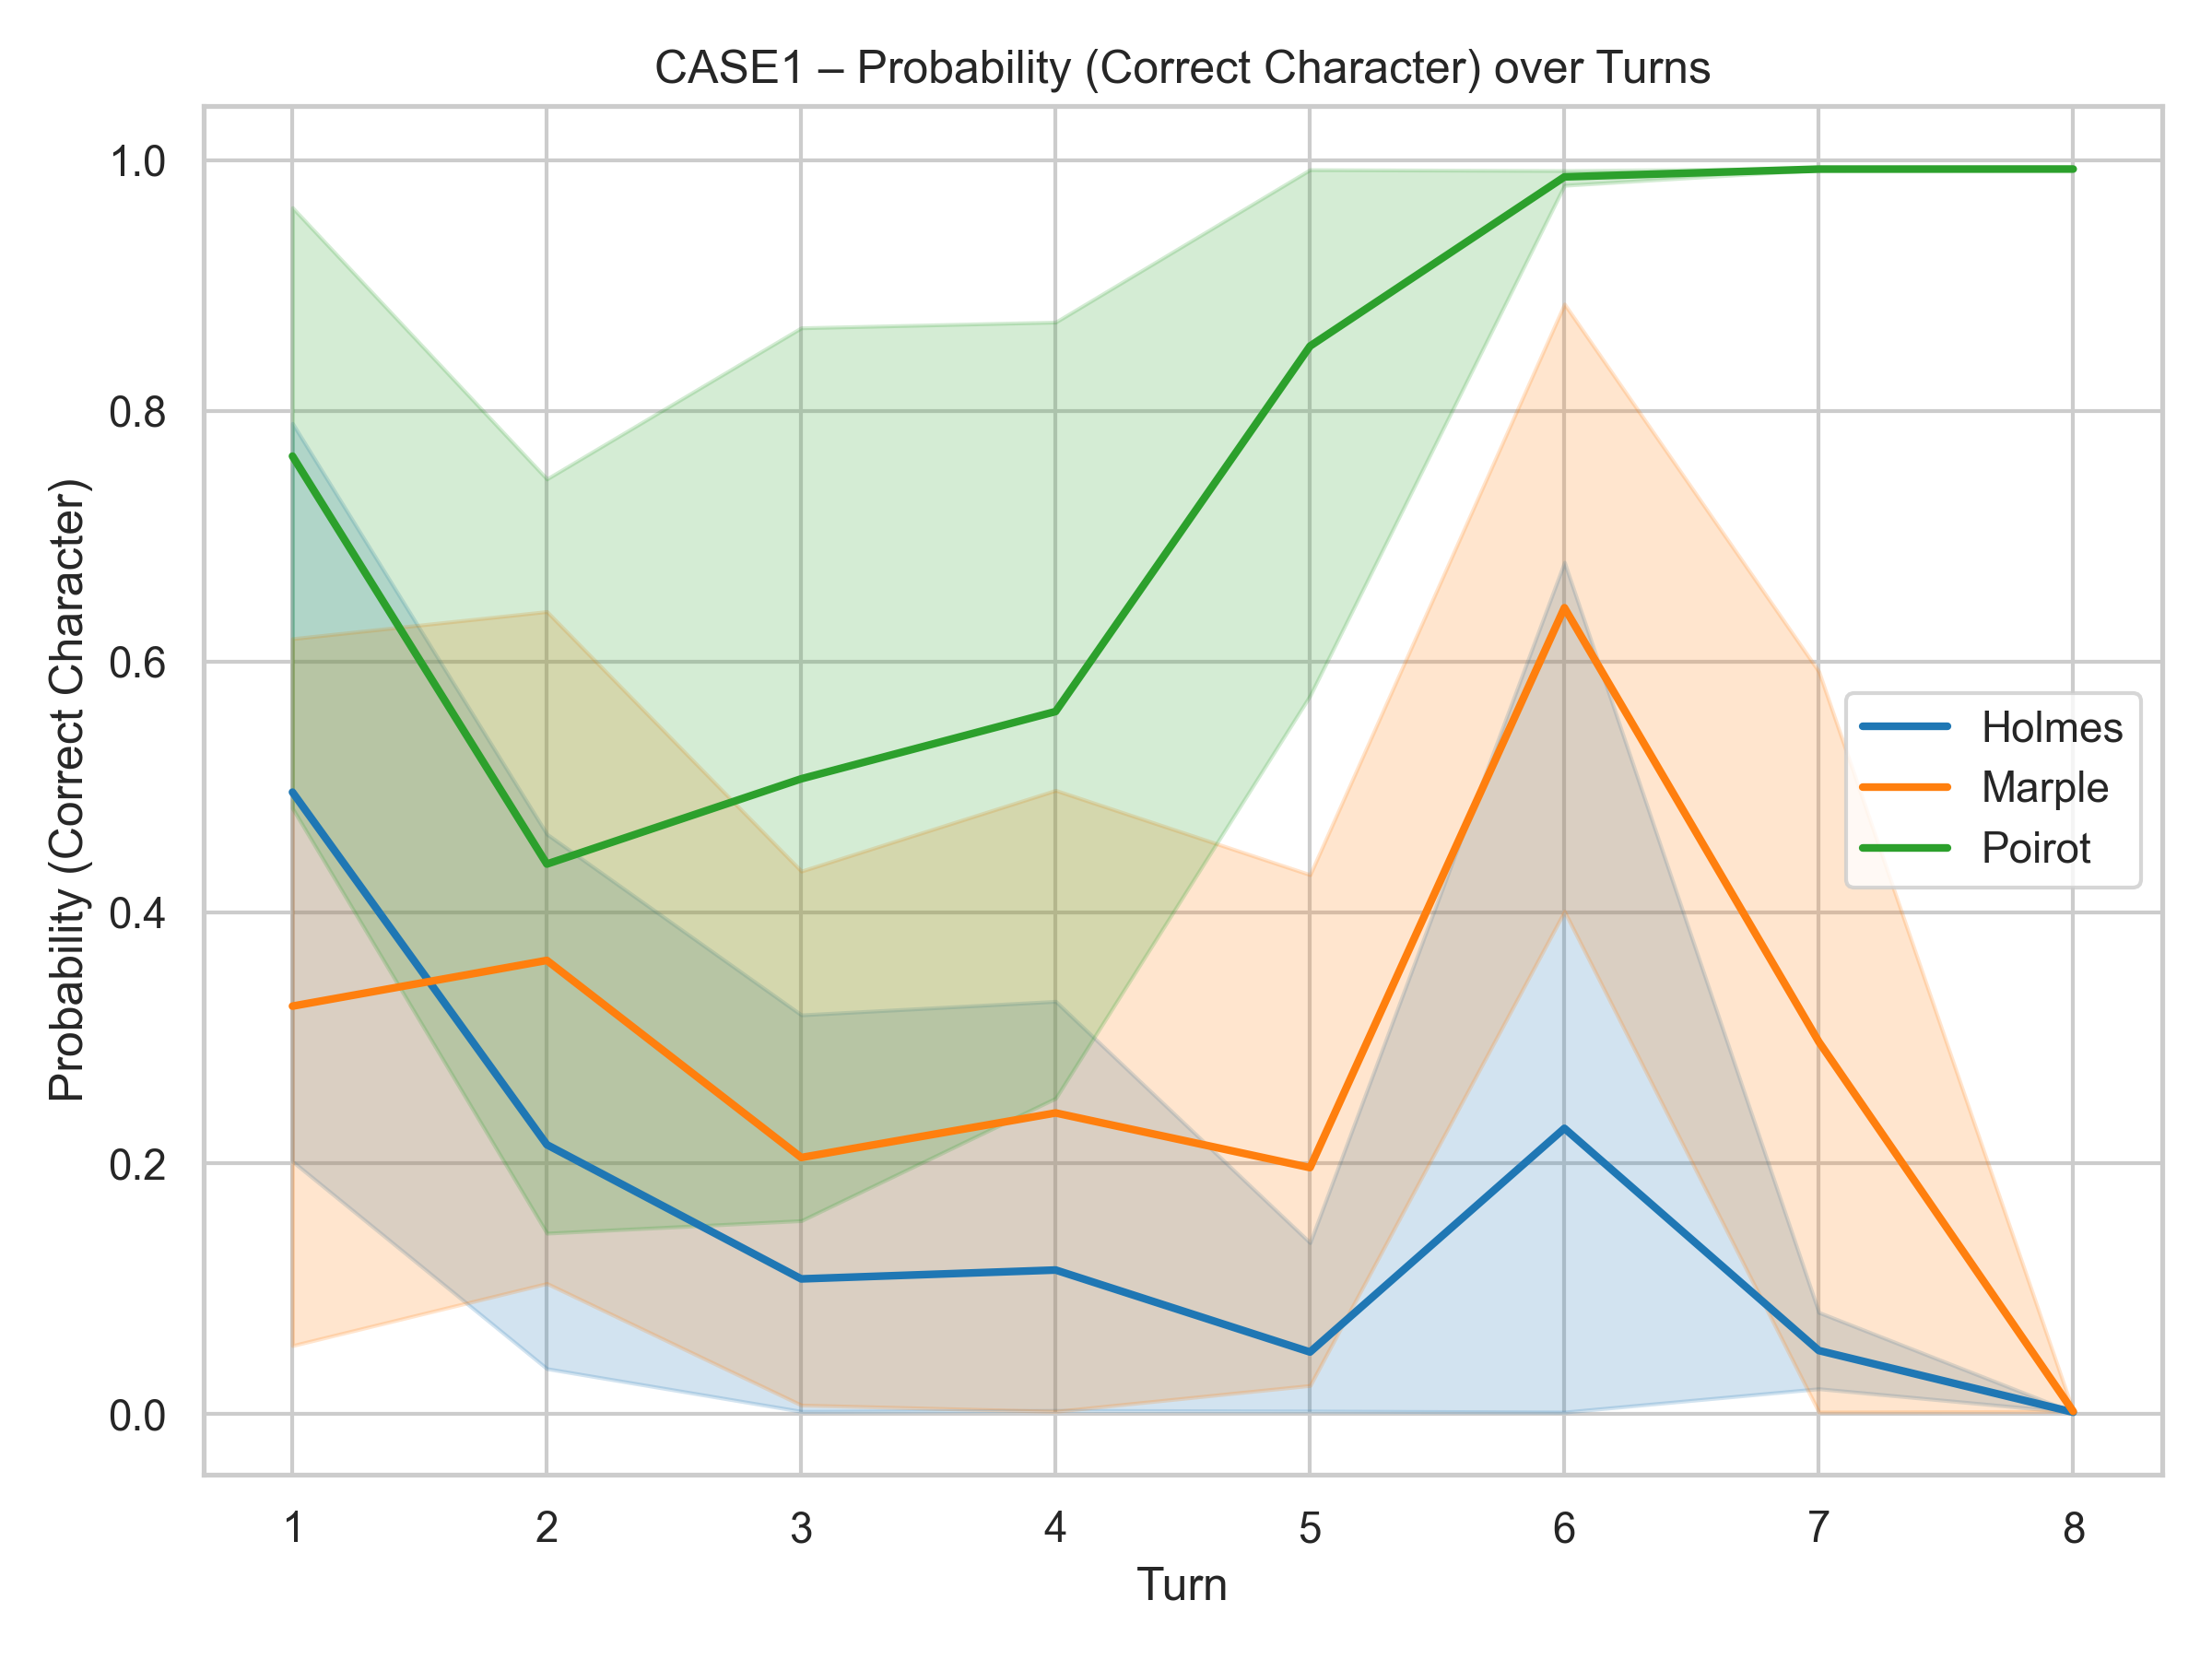
\includegraphics[width=.7\linewidth]{images/case1_prob_multi_agent.png}
            \caption{Predicted Probability}\label{fig:prob_case1}
        \end{subfigure}\qquad
        \begin{subfigure}[b]{1.2\textwidth}
            \centering
            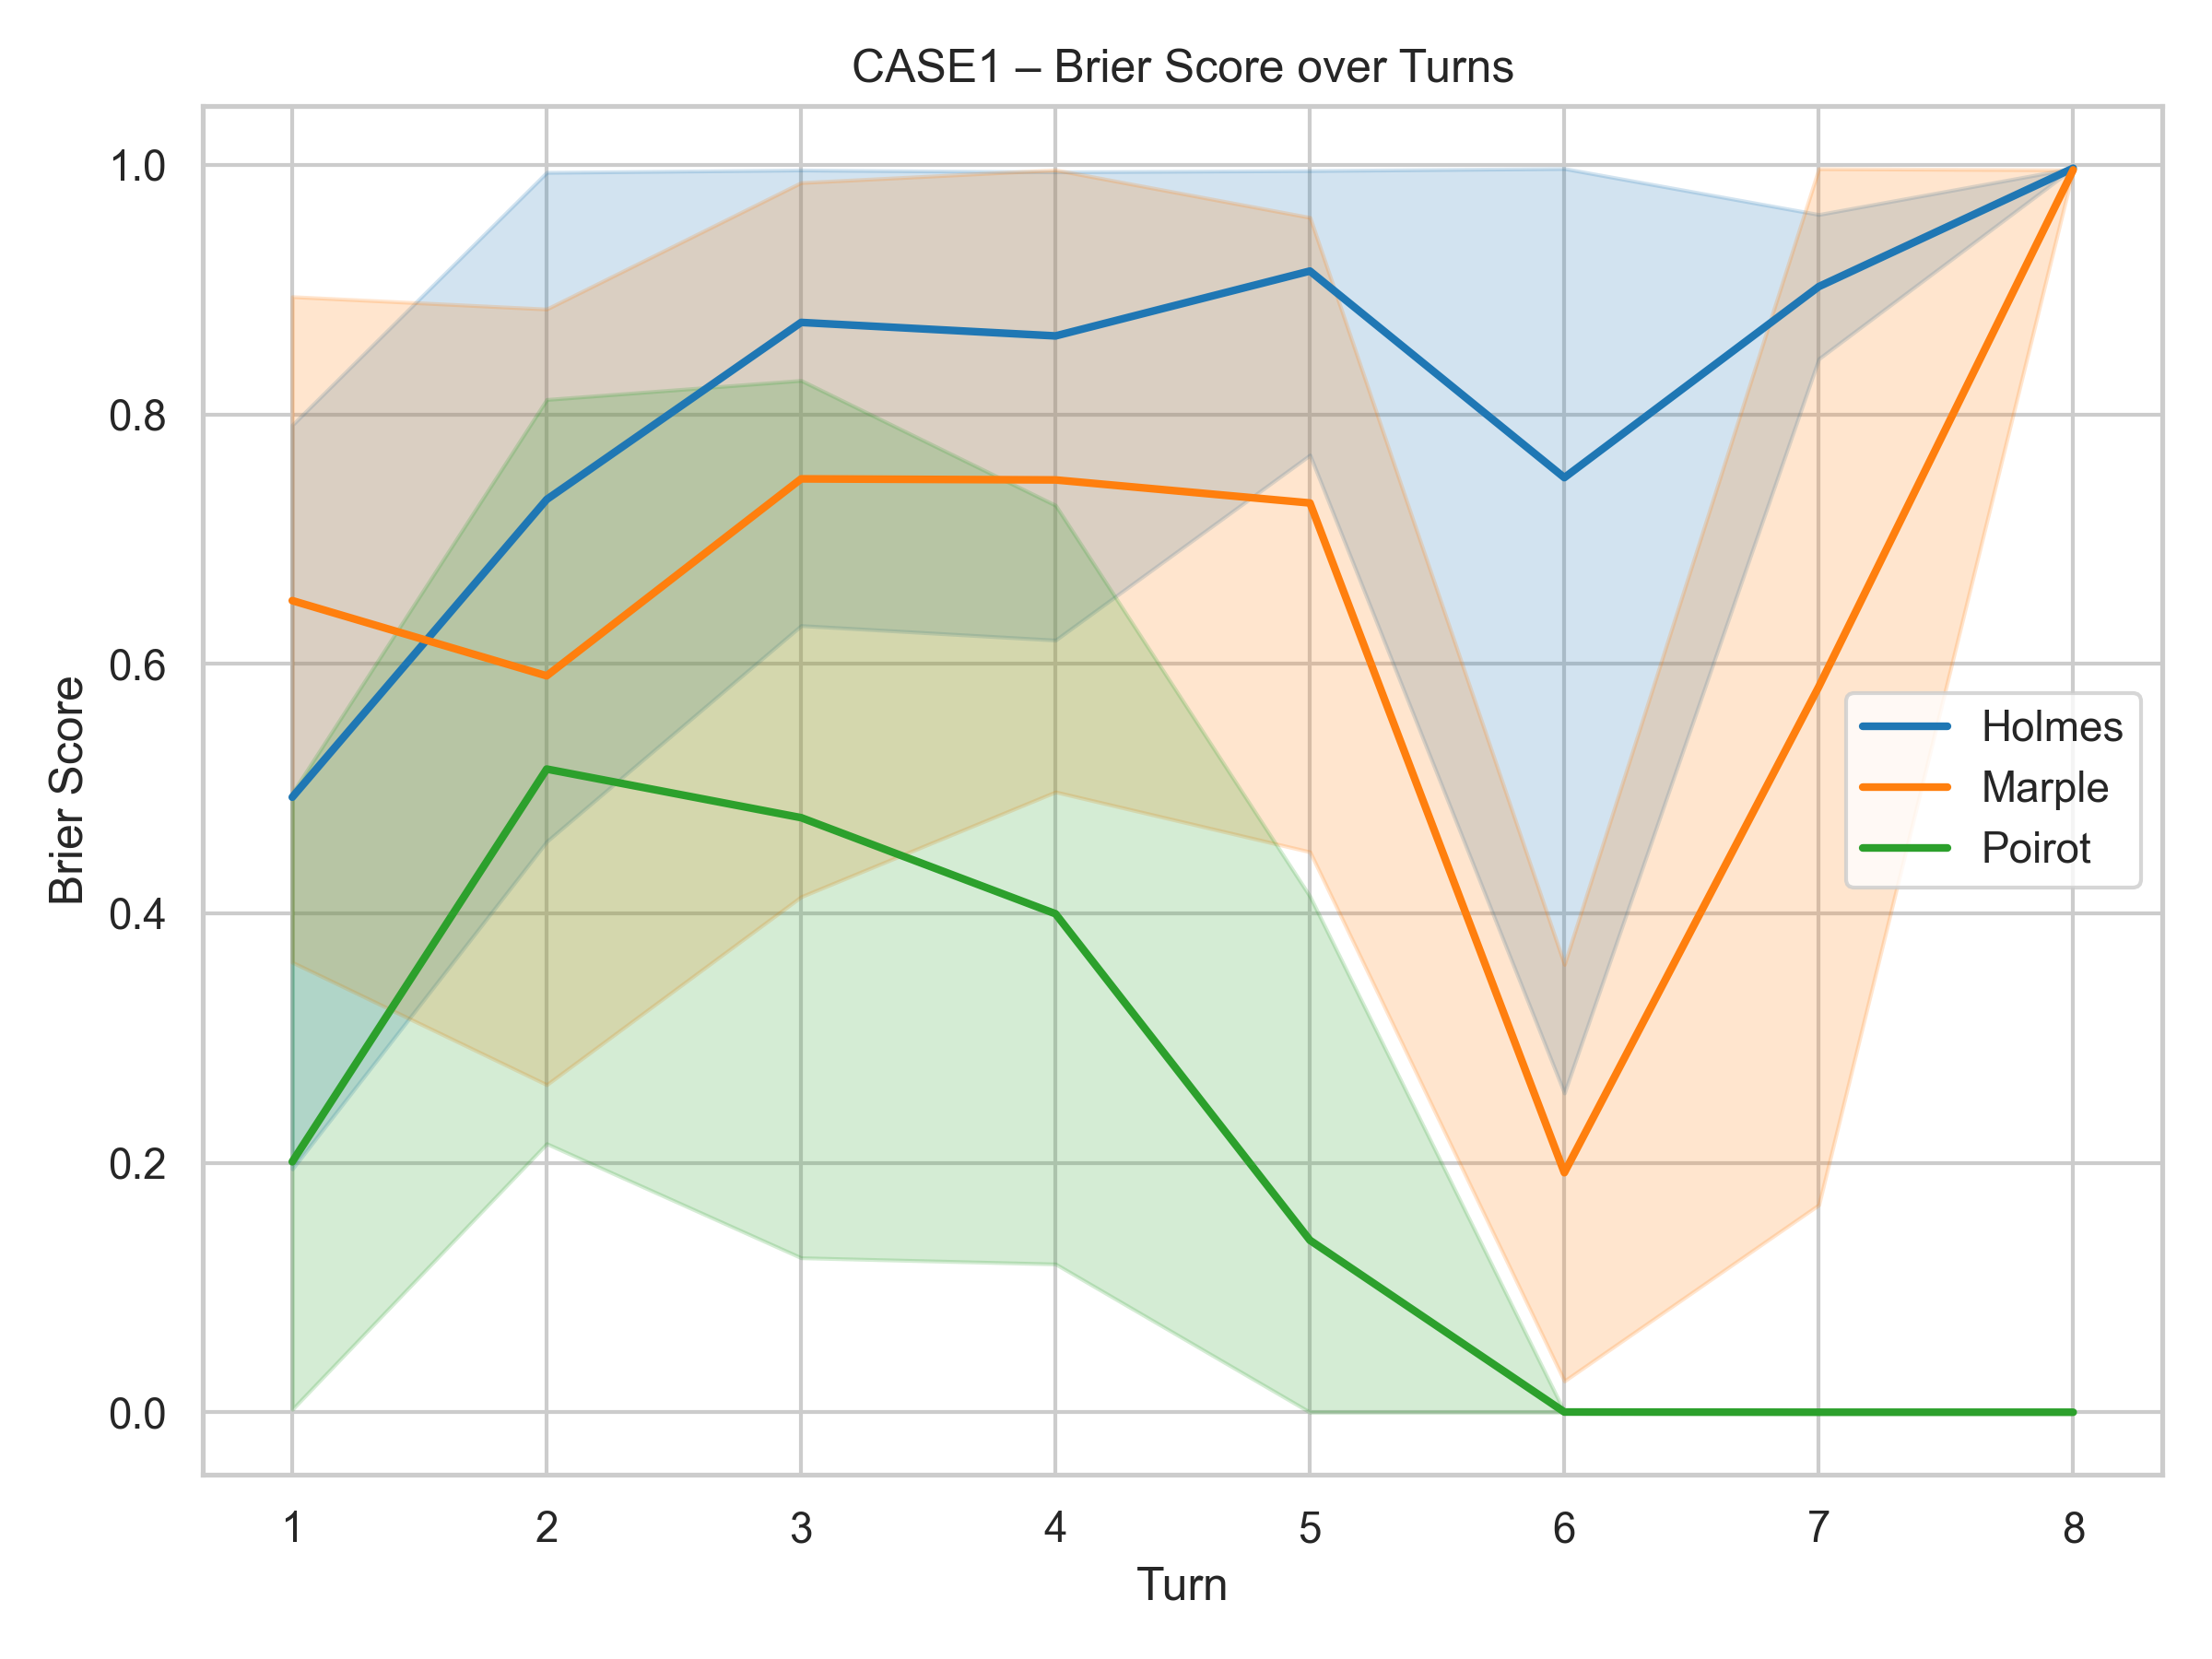
\includegraphics[width=.7\linewidth]{images/case1_brier_multi_agent.png}
            \caption{Brier Score}\label{fig:brier_case1}
        \end{subfigure}
    \caption{Plot of Predicted Probability and Brier Score for Case 1}
    \label{fig:classifier_case1}
    \end{minipage}
\end{figure}

\begin{figure}[H]
    \centering
    \begin{minipage}{\textwidth}
        \centering
        \begin{subfigure}[b]{1.2\textwidth}
            \centering
             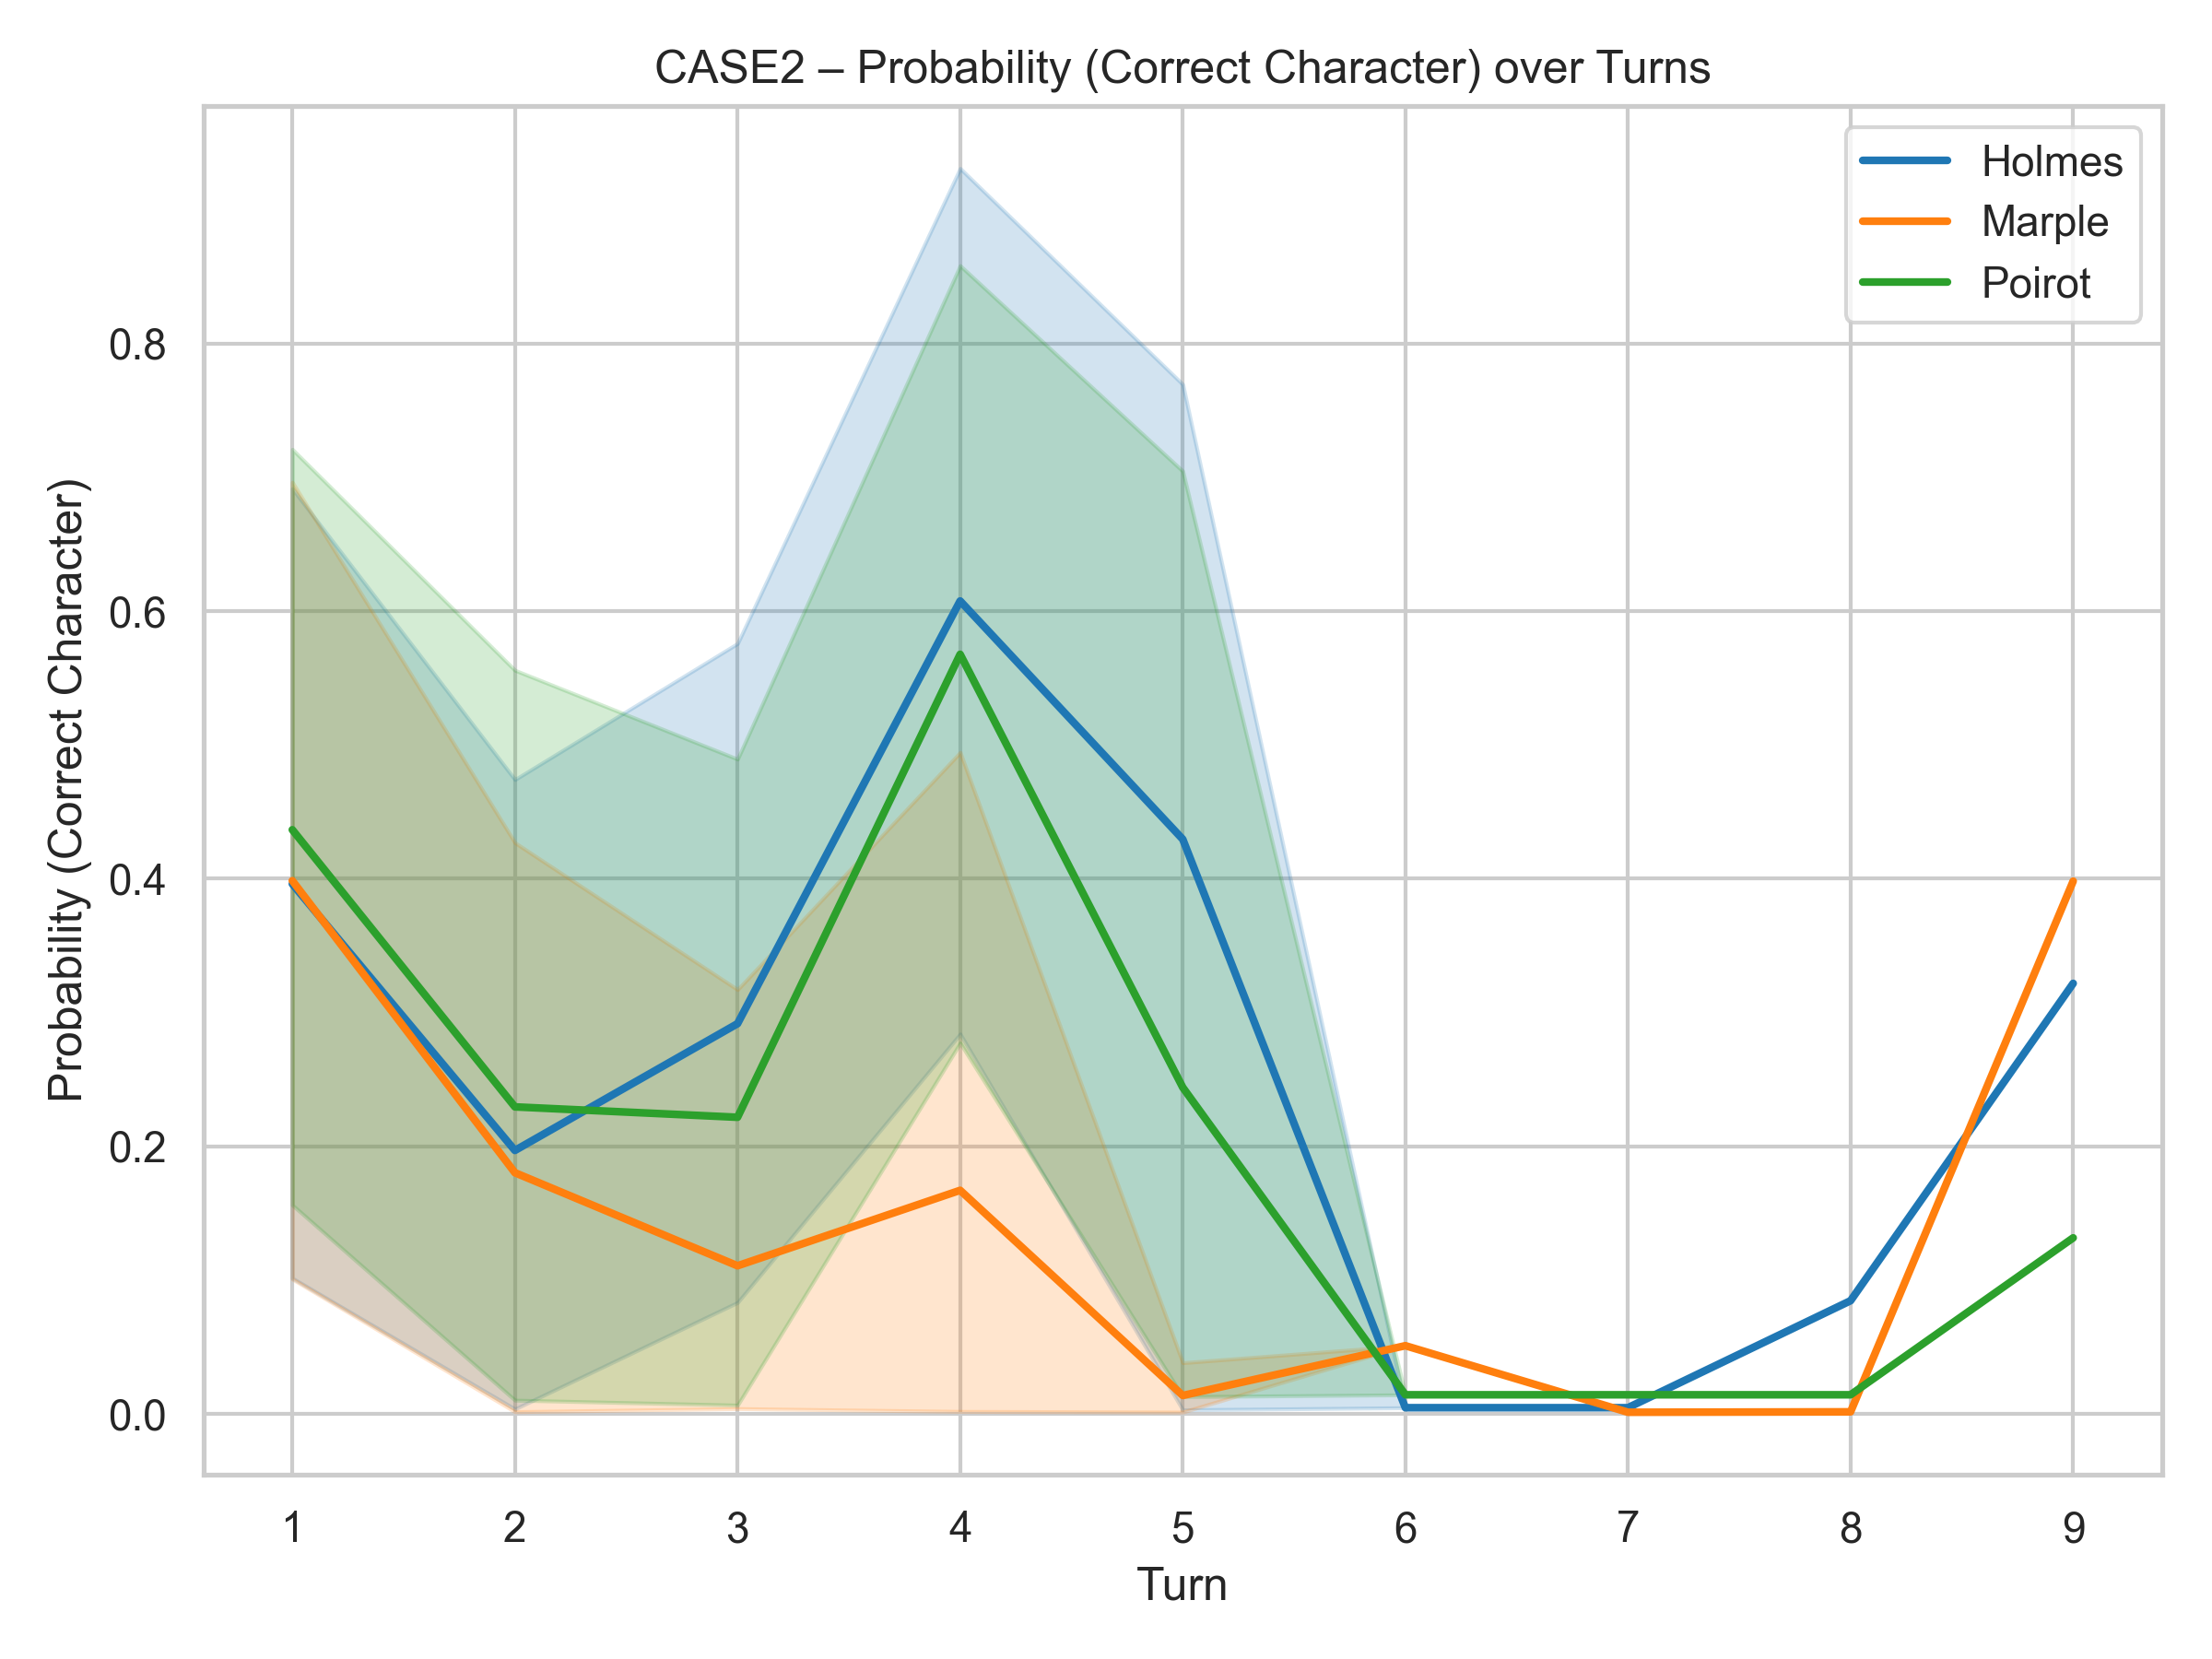
\includegraphics[width=.7\linewidth]{images/case2_prob_multi_agent.png}
            \caption{Predicted Probability}\label{fig:prob_case2}
        \end{subfigure}\qquad
        \begin{subfigure}[b]{1.2\textwidth}
            \centering
            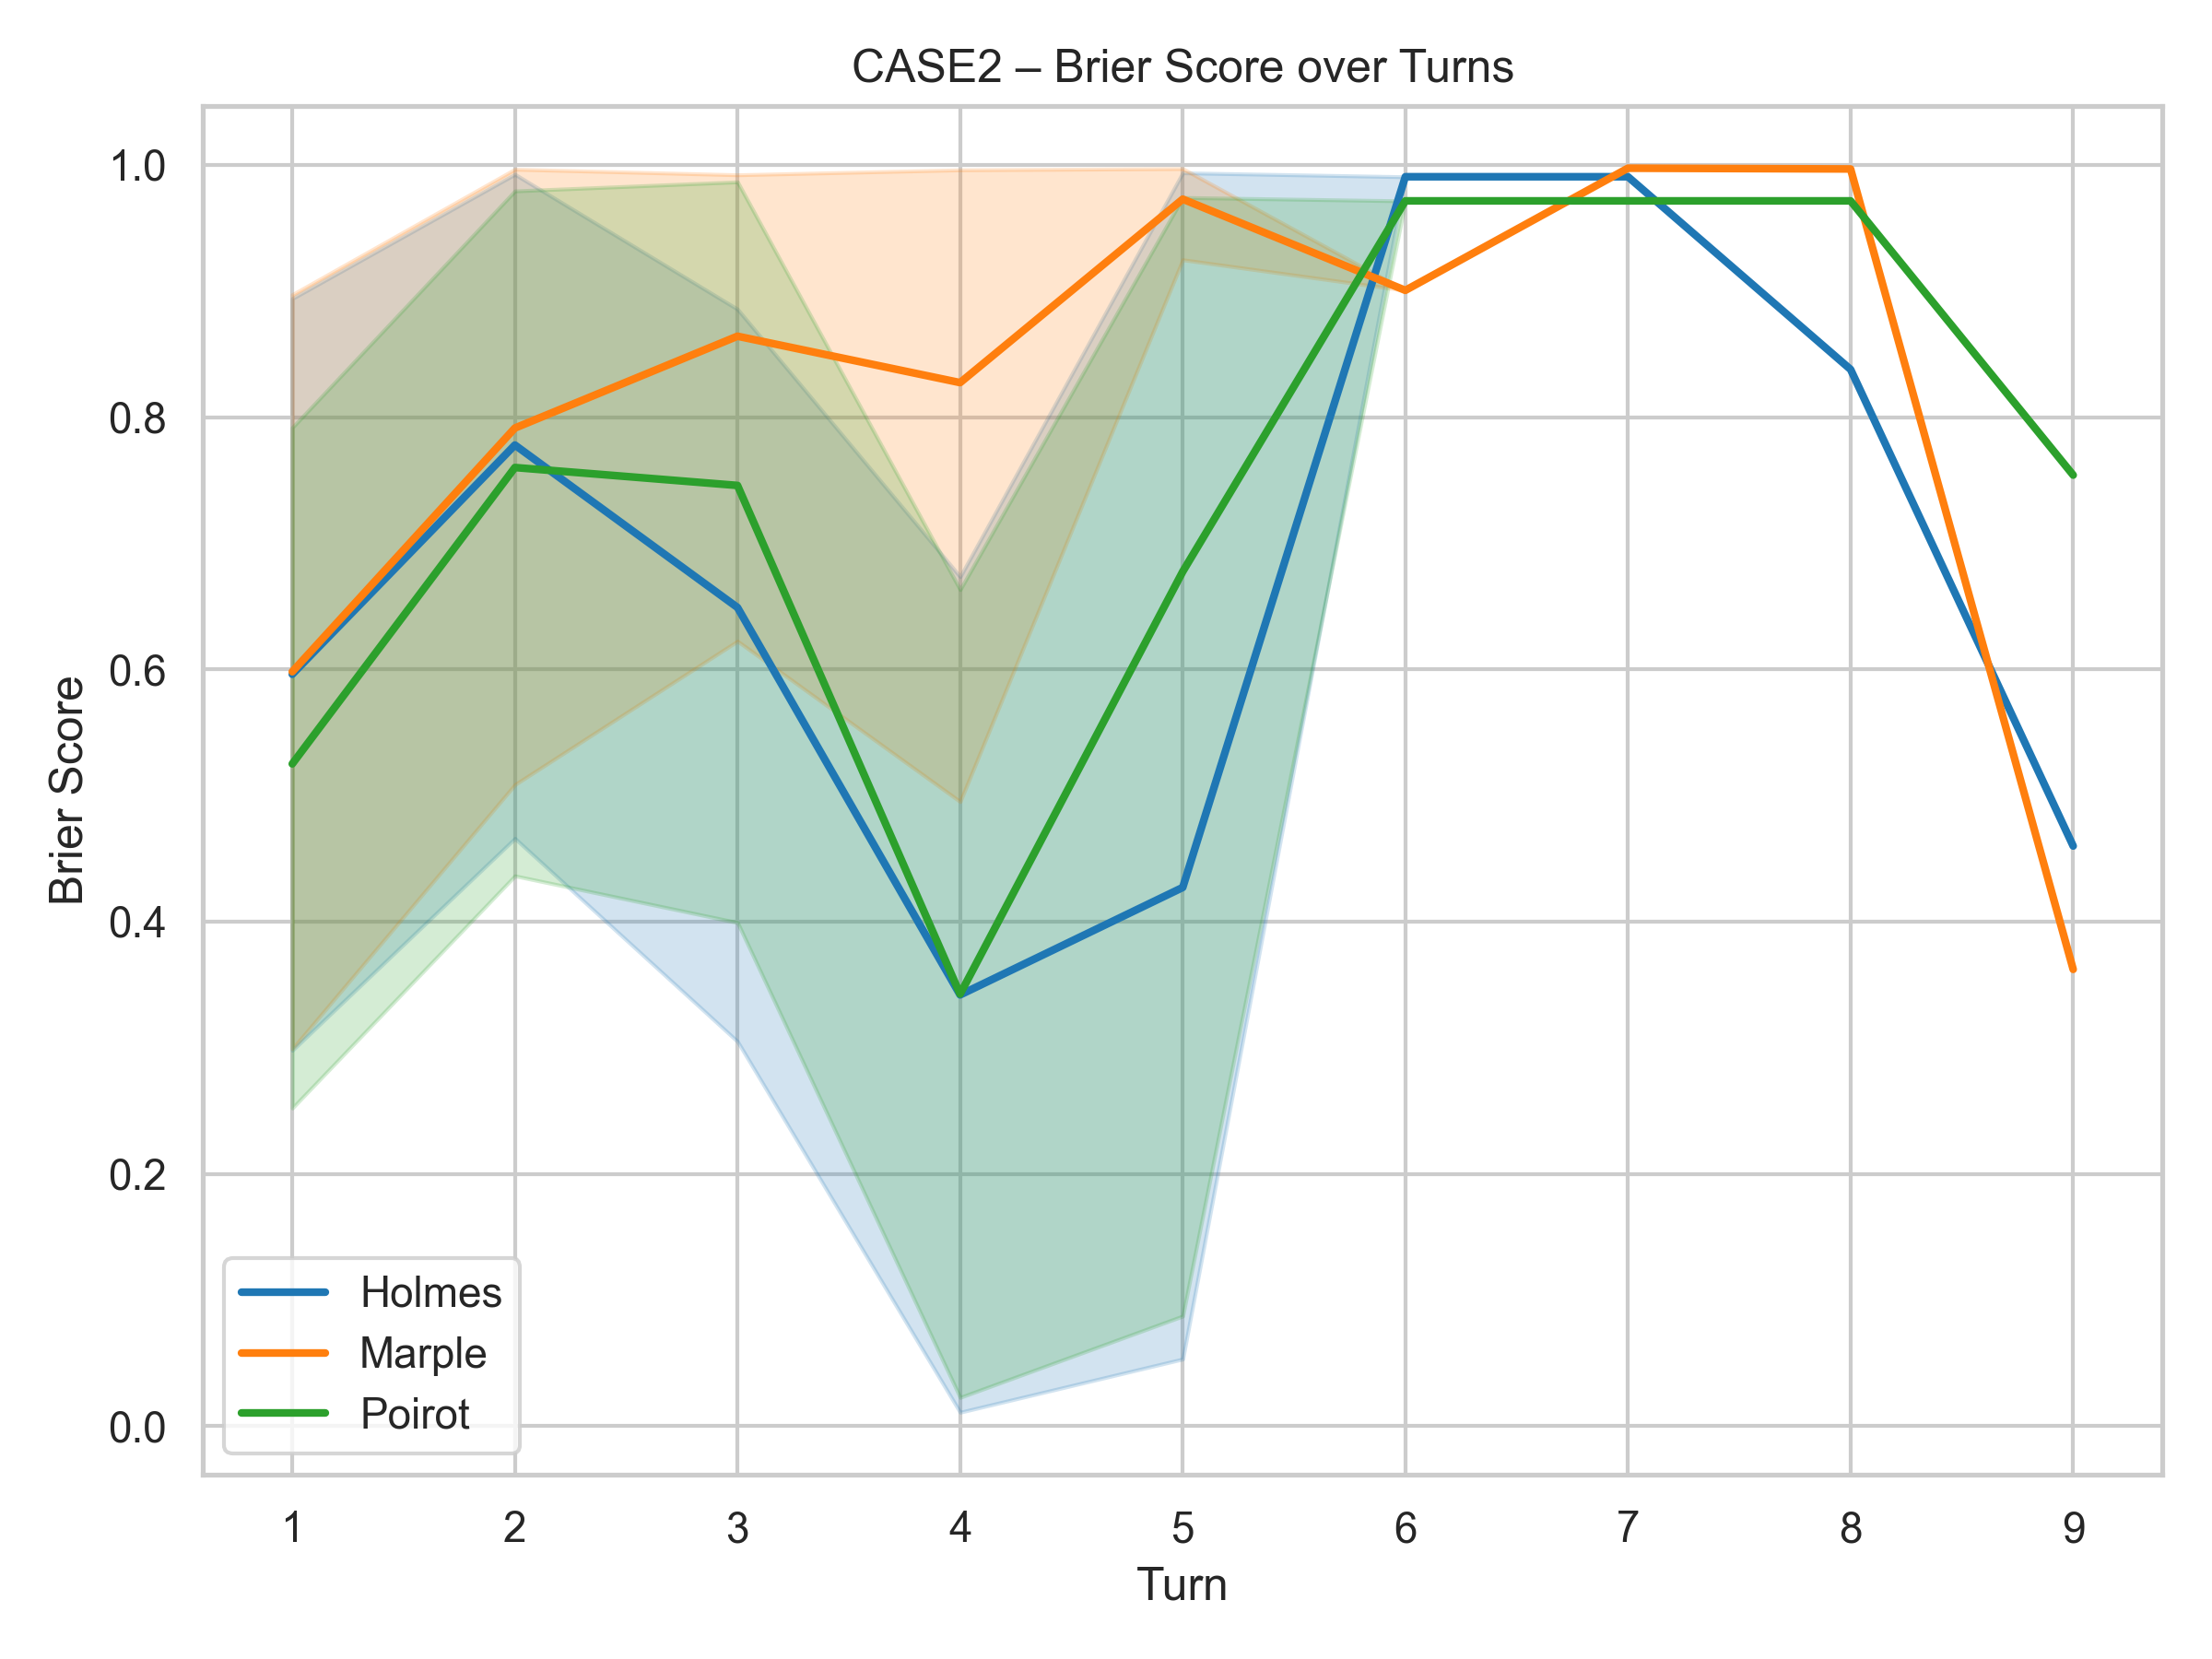
\includegraphics[width=.7\linewidth]{images/case2_brier_multi_agent.png}
            \caption{Brier Score}\label{fig:brier_case2}
        \end{subfigure}
    \caption{Plot of Predicted Probability and Brier Score for Case 2}
    \label{fig:classifier_case2}
    \end{minipage}
\end{figure}

\begin{figure}[H]
    \centering
    \begin{minipage}{\textwidth}
        \centering
        \begin{subfigure}[b]{1.2\textwidth}
            \centering
             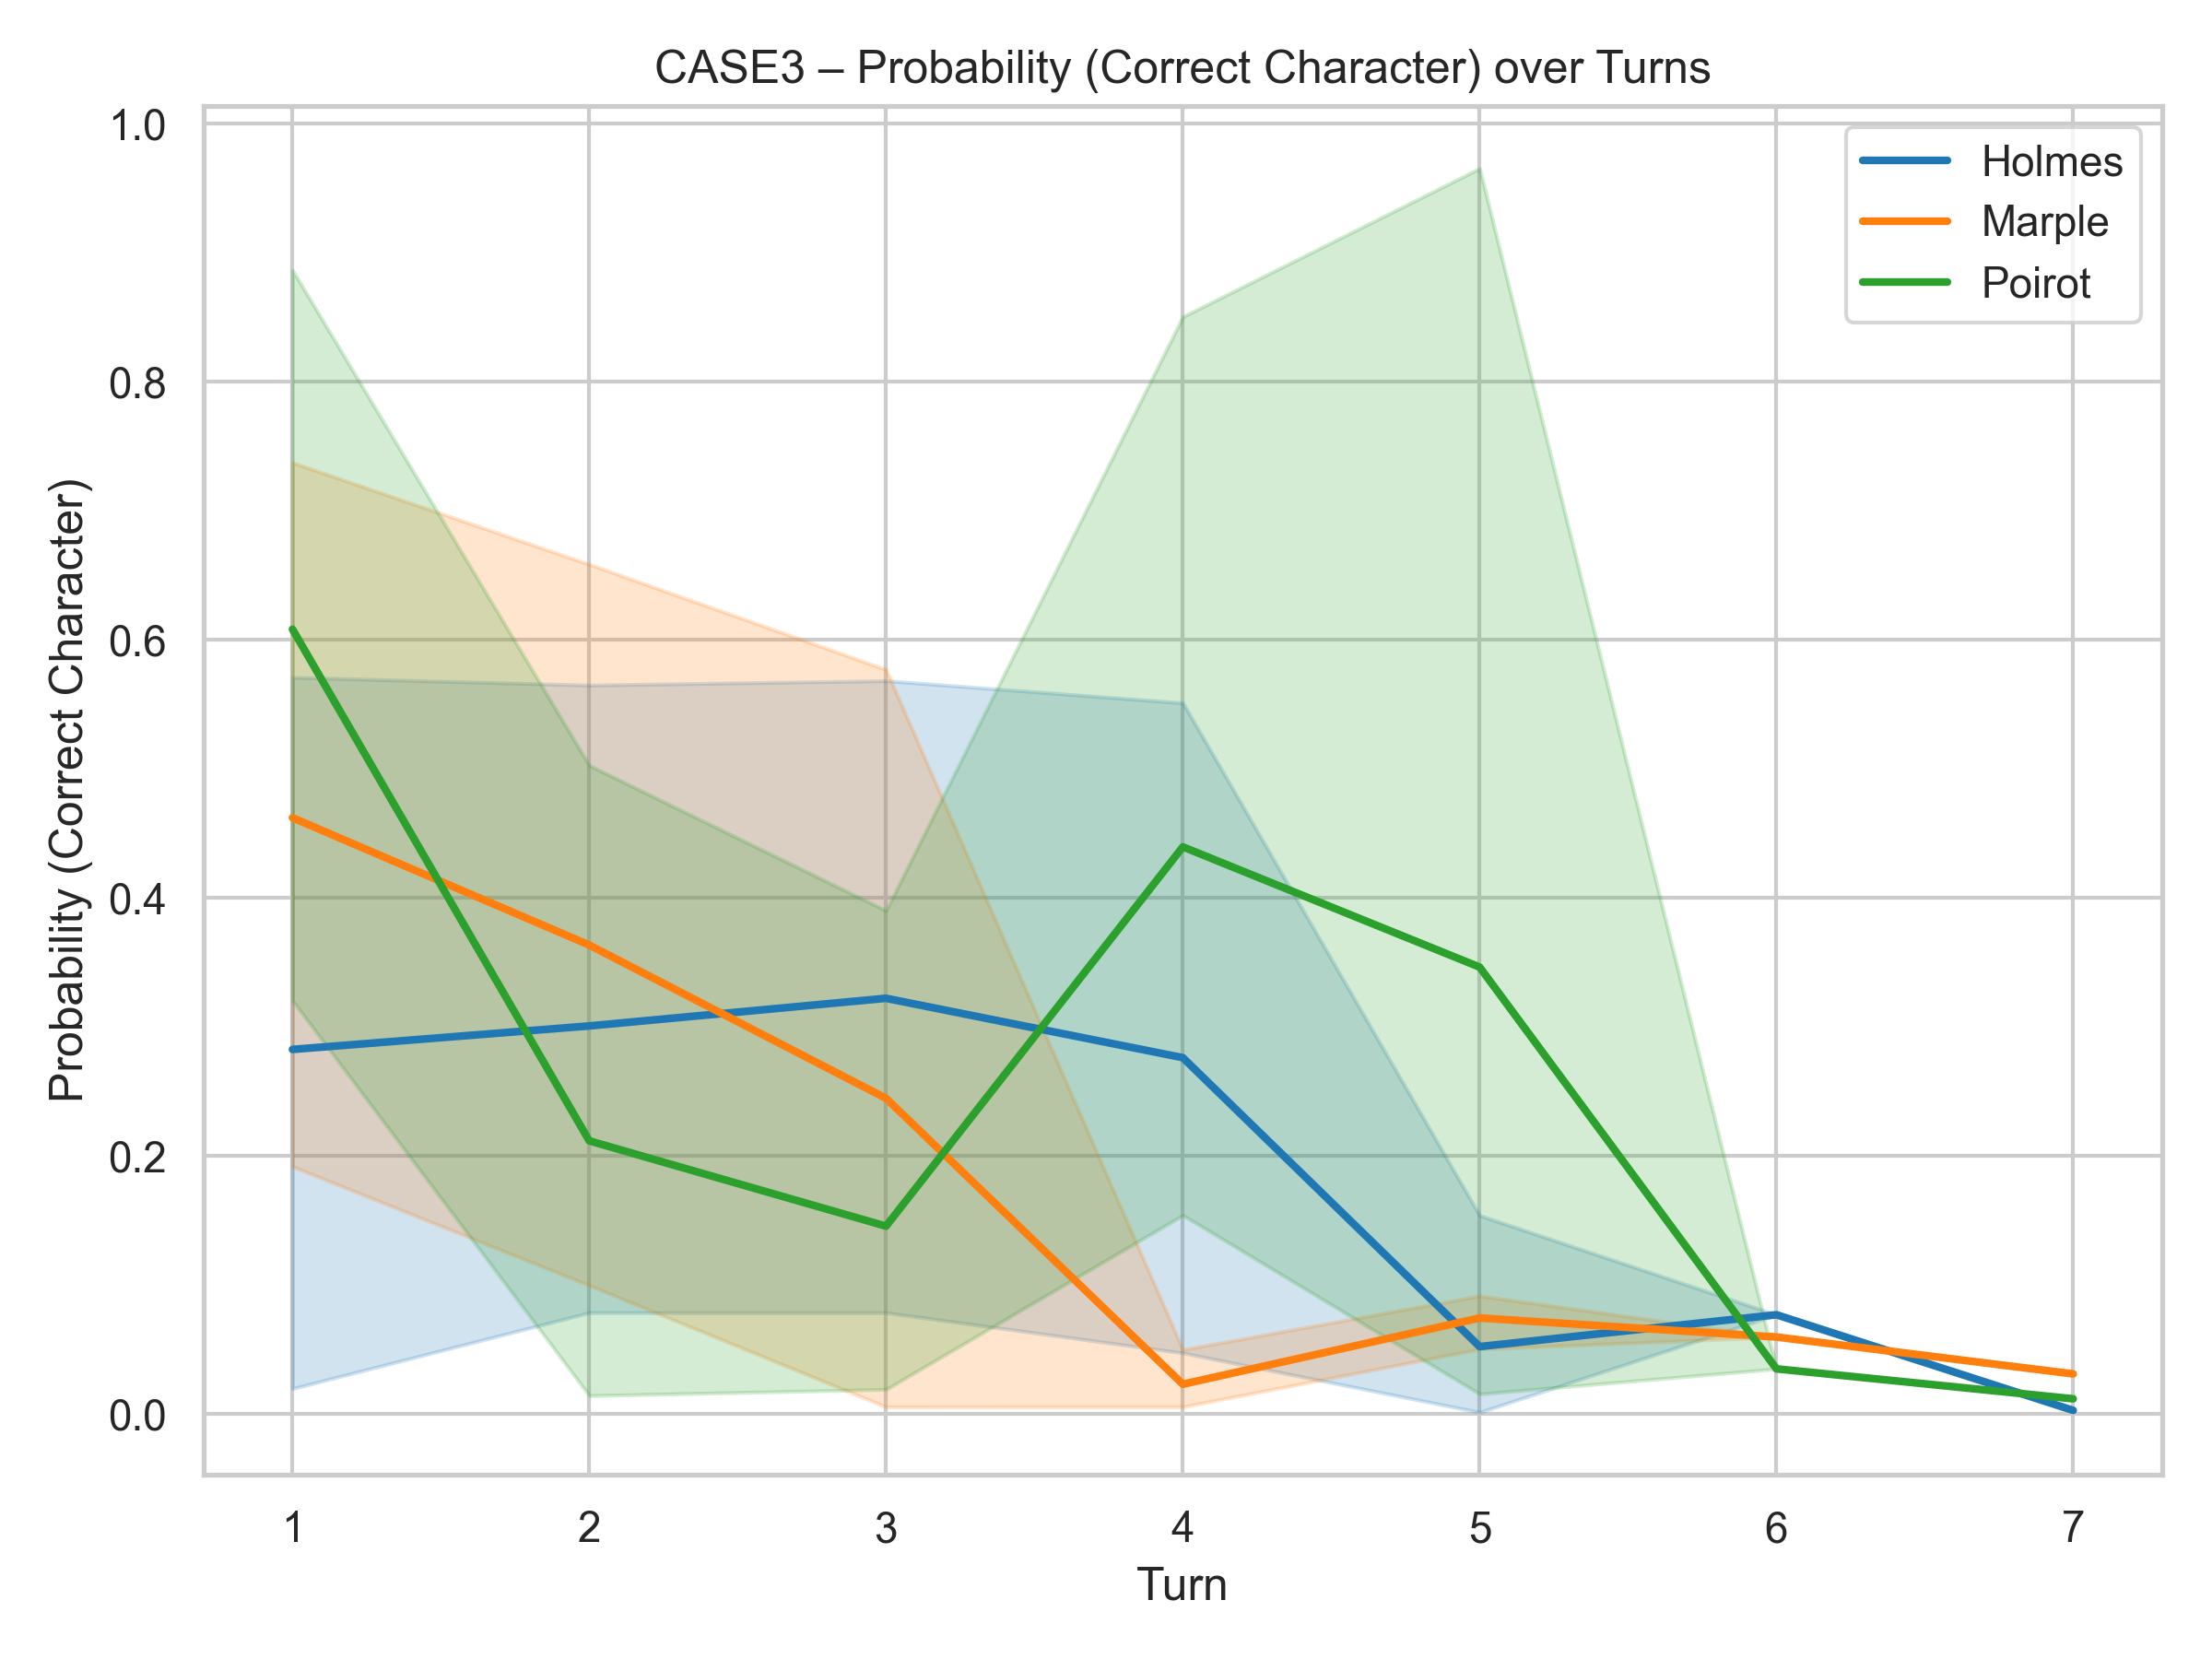
\includegraphics[width=.7\linewidth]{images/case3_prob_multi_agent.png}
            \caption{Predicted Probability}\label{fig:prob_case3}
        \end{subfigure}\qquad
        \begin{subfigure}[b]{1.2\textwidth}
            \centering
            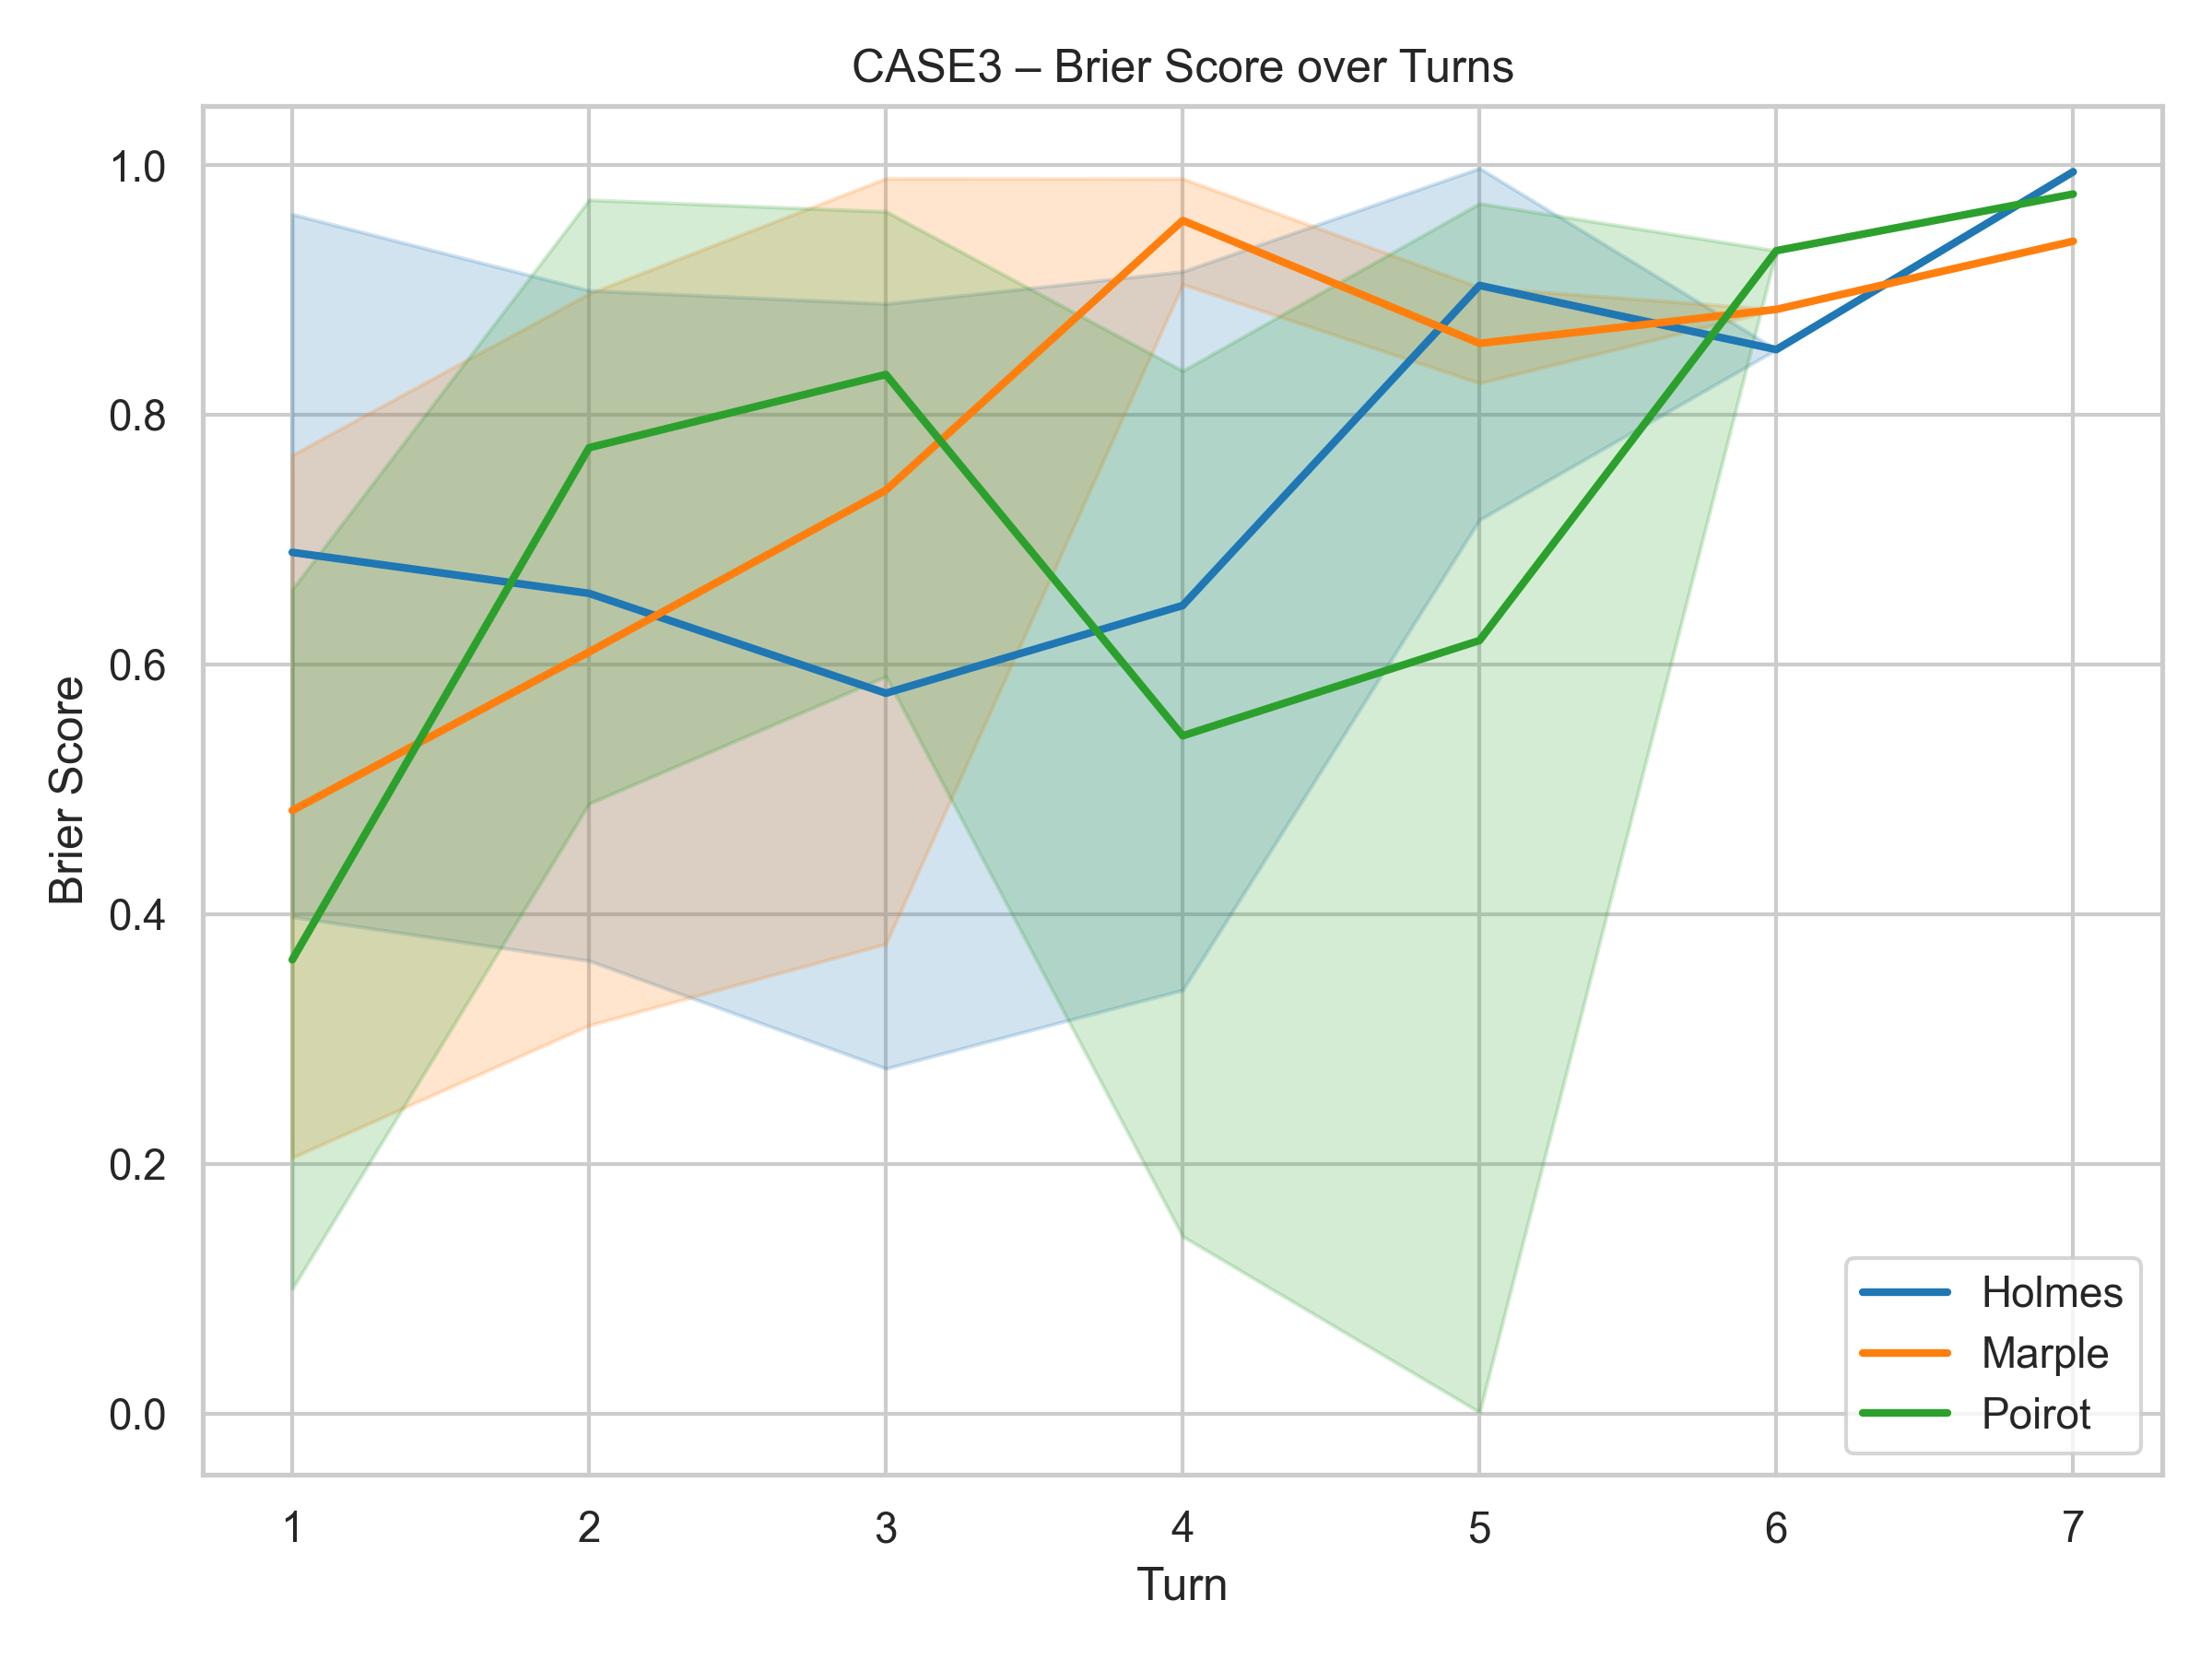
\includegraphics[width=.7\linewidth]{images/case3_brier_multi_agent.png}
            \caption{Brier Score}\label{fig:brier_case3}
        \end{subfigure}
    \caption{Plot of Predicted Probability and Brier Score for Case 3}
    \label{fig:classifier_case3}
    \end{minipage}
\end{figure}

Visualisations above are shown for each case in order to preserve the temporal structure of the dialogues. Nevertheless, since the analysis focuses on character-level consistency, the results below are organised by agent.

\subsubsection{Holmes} \label{sec:results_classifier_holmes}

Holmes showed a significant negative temporal trend in Case 1 ($\beta=-0.063$, $p=.025$). This indicated that classifier confidence in correctly attributing Holmes' utterances decreased gradually over turns. Although the slope was moderate in magnitude, the direction was consistent across simulations, suggesting a systematic tendency rather than isolated fluctuations. This pattern provided evidence of Holmes' character inconsistency in Case 1.

In Cases 2 and 3, no significant trend was observed ($p>.05$ in both cases). In Case 2, the slope was slightly negative but not statistically significant. The Brier score slope was also non-significant and close to zero, indicating stable calibration. In Case 3, the slope for predicted probability was again negative but non-significant, and the Brier score slope was non-significant as well. In both cases, classifier confidence and calibration remained comparatively stable across turns, and no consistent directional movement was detectable. These results suggested that Holmes' character consistency depended on contextual factors inherent to the task scenario.

Taken together, Holmes showed evidence of character inconsistency across all three cases in terms of the overall direction of change: all three regression slopes for predicted probability were negative, indicating a general tendency toward declining classifier confidence and thus failing to maintain consistent persona throughout the dialogues. This negative direction was significant and clear only in Case 1, while in Cases 2 and 3 the downward tendencies were weak and unstable. Nevertheless, the consistent negative direction across cases suggests that Holmes did not consistently sustain his character identity under the interaction conditions tested. The significant increase in Brier score in Case 1 further confirmed reduced probabilistic calibration alongside declining confidence, reinforcing the conclusion of character inconsistency in that case.

\subsubsection{Marple} \label{sec:results_classifier_marple}

For Marple, no significant temporal effects were observed in Cases 1 and 2 for predicted probability (both $p>.50$), and slopes were close to zero. The Brier score slopes in these cases were also non-significant, indicating stable calibration. Classifier confidence remained largely stable across dialogue turns, indicating consistent behavioural recognisability within those scenarios. Minor numerical fluctuations did not suggest a consistent directional trend.

In Case 3, however, a statistically significant negative trend emerged for predicted probability ($\beta=-0.102$, $p=.015$). The magnitude of this slope exceeded that observed for Holmes in Case 1, indicating a comparatively stronger temporal decline in attribution confidence. At the same time, the Brier score showed a significant positive slope ($\beta=-0.103$, $p=.05$), reflecting increasing calibration error as the dialogue unfolded. This suggested that Marple's generated dialogue increasingly diverged from the classifier's learned representation of her persona over time.

Taken together, Marple showed evidence of character inconsistency in Case 3, but not in Cases 1 or 2. In Case 3, the significant negative slope for predicted probability and the significant positive slope for Brier score together indicated declining classifier confidence and worsening calibration, which are direct signs of character inconsistency. In Cases 1 and 2, both metrics remained stable, with non-significant slopes and no consistent directional change. This pattern shows that Marple maintained consistent character identity in Cases 1 and 2, but failed to do so in Case 3.

\subsubsection{Poirot} \label{sec:results_classifier_poirot}

Across all three cases, Poirot did not exhibit statistically significant negative drift in predicted probability (all $p>.09$). In Case 1, a marginal positive trend was observed ($\beta=0.057$, $p=.091$), suggesting a slight increase in classifier confidence over turns. Although this effect did not reach statistical significance, its direction contrasted with the declining patterns observed for Holmes and Marple in their respective drift cases. The Brier score slopes in all three cases were non-significant and close to zero, indicating stable calibration throughout.

In Cases 2 and 3, slopes for predicted probability were close to zero and non-significant, and classifier confidence remained stable across turns. Brier score slopes were also non-significant in these cases. While small numerical fluctuations were present, they did not indicate a systematic temporal decline in either confidence or calibration.

Overall, Poirot maintained consistent character identity throughout the dialogues compared to Holmes and Marple, with no evidence of systematic degradation in classifier confidence or probabilistic calibration

\subsubsection{Classifier Results Summary} \label{sec:results_classifier_summary}

Across characters and cases, classifier-based character consistency was generally stable. Statistically significant temporal inconsistency was observed in only two instances: Holmes in Case 1 and Marple in Case 3. In both cases, the predicted probability of the correct class decreased significantly over turns, accompanied by a significant increase in Brier score. This pattern indicated both declining attribution confidence and reduced probabilistic calibration as the dialogue progressed, providing clear evidence of character inconsistency in these two character-case combinations. Overall, the results suggested that character inconsistency emerged selectively rather than systematically.

\subsection{Lexical metrics} \label{sec:results_lexical}

As introduced in Subsection \ref{sec:eval_lexical}, from the lexically perspective this study examines how closely each generated utterance matches the character's established vocabulary, using TF-IDF cosine similarity to the gold reference corpus. It also compares similarity within the same agent over time against similarity across different agents at the same turn. The resulting character distance score indicates whether lexical patterns are driven by character identity or by shared conversational content. Kruskal-Wallis and Mann-Whitney $U$ tests are used to assess whether lexical similarity differs across characters, and to identify which specific pairs show significant differences.

To ensure data quality, simulated utterances were pre-filtered to a minimum length of 6 tokens, resulting in 129 simulated utterances per character. For the reference corpus, a fixed sample of 100 baseline utterances per character was randomly selected (seed = 42) from the full corpus. This sampling strategy was chosen for keeping a balance between computational efficiency and maintainance of a sufficiently diverse lexical basis. Because simulated utterances are evaluated against these reference sets independently, the difference in sample size between baseline ($n=100$ per character) and simulation data ($n=129$ per character) introduces little statistical imbalance.

\subsubsection{Character-specific vocabulary similarity} \label{sec:results_lexical_vocab}

Table \ref{tab:lexical_tfidf} presents summary statistics of cosine similarity between simulated utterances and character-specific TF-IDF representations from the reference corpus. Poirot shows the highest mean similarity ($M=0.119$, $SD=0.025$), followed by Marple ($M=0.110$, $SD=0.041$) and Holmes ($M=0.100$, $SD=0.025$). Although absolute values are modest, the differences suggest variation in how closely each character aligns with their canonical vocabulary.

\begin{table}[H]
\centering
\begin{tabular}{l l l l l}\toprule
Character & Cosine Mean& Cosine SD& Cosine Min & Cosine Max \\\midrule
Holmes & 0.100 & 0.025 & 0.047 & 0.175 \\
Marple & 0.110 & 0.041 & 0.042 & 0.263 \\
Poirot & 0.119 & 0.025 & 0.064 & 0.184 \\ \bottomrule
\end{tabular}
\caption{Summary of TF-IDF similarity statistics.}
\label{tab:lexical_tfidf}
\end{table}

A Kruskal-Wallis test confirmed a significant effect of character identity on TF-IDF similarity ($H(2)=30.11$, $p<.001$) (Table \ref{tab:lexical_stattest}), indicating that the distributions differ across characters. Bonferroni-corrected pairwise Mann-Whitney $U$ tests show that Poirot has significantly higher similarity than both Holmes ($U=4844.0$, $p<.001$) and Marple ($U=6413.0$, $p=.001$), while the difference between Holmes and Marple is not significant ($U=7504.0$, $p=.173$). 

\begin{table}[H]
\centering
\begin{tabular}{l l l l l}\toprule
Test Type & Comparison / Test & Test Statistic & df & $p$-value \\\midrule
Overall & Kruskal-Wallis & $H=30.11$*** & 2 & < .001 \\
Pairwise & Holmes vs Marple & $U=7504.0$ & - & .173 \\
Pairwise & Holmes vs Poirot & $U=4844.0$*** & - & < .001 \\
Pairwise & Marple vs Poirot & $U=6413.0$** & - & .001 \\ \bottomrule
\end{tabular}
\caption{Kruskal-Wallis and pairwise Mann-Whitney $U$ test results (Bonferroni corrected).}
\label{tab:lexical_stattest}
\end{table}

Beyond mean differences, variability also differs across characters. Marple shows the largest spread ($SD=0.041$, range: 0.042-0.263), suggesting less stable lexical alignment, whereas Holmes and Poirot are more concentrated. Overall, all agents show some degree of character consistency from lexical perspective, but Poirot demonstrates the strongest and most stable alignment with the reference vocabulary.

\subsubsection{Character distance (intra- vs. cross-agent similarity)}  \label{sec:results_lexical_chardistance}

This analysis examines whether lexical similarity is primarily driven by character identity or by shared conversational content. Following Subsection \ref{sec:eval_lexical}, intra-agent and cross-agent similarities are computed within each simulation run, and their difference (character distance) is used as the main indicator. More specifically, positive values indicate that an agent's lexical choices are more similar to its own previous utterances than to those of other agents, reflecting character-specific consistency. All similarities are computed within a shared TF-IDF space over generated utterances to ensure comparability. Since intra-agent similarity requires a previous utterance, the first turn of each run is excluded.

Positive values indicate that lexical persistence is driven by character identity rather than shared conversational content. This metric was computed within a shared TF-IDF embedding space built over all generated utterances to ensure direct comparability. Due to the lag required for transition values, the first utterance of each run was excluded from the analysis.

Table \ref{tab:lexical_char_distance} summarises intra-agent similarity, cross-agent similarity, and their difference. For all characters, intra-agent similarity is slightly higher than cross-agent similarity, but the magnitude of this difference varies. Poirot and Holmes show clear positive character distance (Poirot: $M=0.075$, Holmes: $M=0.069$), indicating that their lexical patterns remain more aligned with their own prior speech than with the group. In contrast, Marple's mean distance is close to zero ($M=0.005$), suggesting little distinction from the shared dialogue. For Marple, intra- and cross-agent similarities are nearly identical, which explains the near-zero character distance.

Overall, the results show that Poirot and Holmes retain a stable lexical fingerprints under collaboration, whereas that of Marple's is largely shaped by the shared conversational context.

\begin{table}[H]
\centering
\begin{tabular}{l l l l l}\toprule
Character & Intra Mean & Cross Mean & Distance Mean & Distance SD \\\midrule
Holmes & 0.357 & 0.288 & 0.069 & 0.219 \\
Marple & 0.279 & 0.274 & 0.005 & 0.194 \\
Poirot & 0.370 & 0.295 & 0.075 & 0.221 \\ \bottomrule
\end{tabular}
\caption{Summary of intra-agent similarity, cross-agent similarity, and their difference (character distance).}
\label{tab:lexical_char_distance}
\end{table}


\subsubsection{Lexical results summary}

Taken together, the lexical analyses shows that character consistency is present but uneven across agents. Poirot achieves the strongest alignment with his reference vocabulary and maintains clear separation from other agents during interaction. Holmes shows a similar but slightly weaker pattern. In contrast, Marple, despite moderate alignment at the vocabulary level, shows little distinction from the group in interaction, indicating that her lexical behaviour is more influenced by shared conversational context.

These results suggest that lexical character consistency depends not only on alignment with a reference corpus, but also on the ability to sustain that alignment during multi-agent collaboration.

\begin{table}[H]
\centering
\begin{tabular}{l l l}\toprule
Character & TF-IDF Mean & Character Distance Mean \\\midrule
Holmes & 0.100 & 0.069 \\
Marple & 0.110 & 0.005 \\
Poirot & 0.119 & 0.075 \\ \bottomrule
\end{tabular}
\caption{Lexical Consistency Indicators by Character}
\label{lexical_summary}
\end{table}

Poirot exhibited the highest levels of character consistency across both metrics ($M_{TF-IDF}=0.119$; $M_{CharDist}=0.075$). This indicates that he kept the unique lexical features and vocabulary even under the pressure of group interaction. Holmes also maintained a stable lexical fingerprint ($M_{CharDist}=0.069$), showing clear differentiation from the other detectives.

In contrast, Marple showed a clear mismatch: although her average alignment with her literary reference was moderate ($M_{TF-IDF}=0.110$), her character distance was near zero ($M_{CharDist}=0.005$). This shows that her lexical choices were highly susceptible to the collective dialogue flow. Her individual utterances appeared consistent when looked at alone, but her character consistency was more easily eroded during collaborative reasoning. Overall, these findings indicate that lexical character consistency was present but not maintained equally across the three detectives.


\subsection{Syntactic metrics} \label{sec:results_syntactic}

Character consistency was also evaluated at the syntactic level using dependency tree depth as a measure of structural complexity. As introduced in Subsection \ref{sec:eval_syntacic}, three aspects were considered: deviation from literary reference ($z_{\mathrm{ref}}$), internal variability within the simulation ($z_{\mathrm{sim}}$), and temporal trends across dialogue turns.

\subsubsection{Deviation from the reference}

Table \ref{tab:syntax_depth} summarised mean dependency depths for the baseline texts and the simulated dialogue. Across all characters, generated utterances showed substantially higher mean depth than the literary reference (Holmes: +50.99\%, Poirot: +66.70\%, Marple: +73.42\%). In absolute terms, simulation means clustered around 6.8-7.0, whereas baseline means ranged from 4.06 to 4.59.

\begin{table}[H]
\centering
\resizebox{\textwidth}{!}{%
\begin{tabular}{l l l l l l l}
 & \multicolumn{2}{c}{Reference}& \multicolumn{2}{c}{Simulation}& \multicolumn{2}{c}{Difference}\\\toprule
Character& Mean Depth& SD& Mean Depth& SD& Depth Diff.& Increase (\%)\\\midrule
Holmes & 4.588 & 1.693 & 6.928 & 0.742 & 2.339 & 50.99 \\
Marple & 4.057 & 1.339 & 7.035 & 0.744 & 2.979 & 73.42 \\
Poirot & 4.086 & 1.427 & 6.812 & 0.743 & 2.726 & 66.70 \\ \bottomrule
\end{tabular}
}%
\caption{Mean syntactic depth and deviation from literary reference by character}
\label{tab:syntax_depth}
\end{table}

Standard deviations within the simulation (approx. 0.74) are lower than in the literary baselines (1.34-1.69), indicating that the model generates consistently deeper structures rather than simply more variable ones. This shift reflects a global elevation in syntactic complexity, independent of dialogue progression.


\subsubsection{Temporal trends in syntactic deviation}

To examine whether syntactic divergence increases over dialogue turns, linear regressions were run for each character using turn index as predictor and reference-based z-score ($z_{\mathrm{ref}}$) as dependent variable. Table \ref{tab:syntax_regression} showed that all characters exhibit positive slopes, indicating progressive divergence from their literary references. Holmes showed the steepest slope (0.105, $p<.01$), followed by Poirot (0.093, $p<.01$), while Marple's slope (0.078) did not reach conventional significance.

These results indicate a systematic erosion of character consistency over dialogue turns for Holmes and Poirot, with simulated utterances becoming increasingly complex and distant from their literary reference. Marple shows a similar positive trend, but it is less pronounced and not statistically significant.

\begin{table}[H]
\centering
\begin{tabular}{l l l l l}\toprule
Character & $z$ Variant& Slope & $R^2$& Std. Err \\\midrule
Holmes & $z_{\mathrm{ref}}$& 0.105** & 0.189 & 0.019 \\
Holmes & $z_{\mathrm{sim}}$& 0.240** & 0.189 & 0.044 \\
Marple & $z_{\mathrm{ref}}$& 0.078 & 0.065 & 0.026 \\
Marple & $z_{\mathrm{sim}}$& 0.140 & 0.065 & 0.047 \\
Poirot & $z_{\mathrm{ref}}$& 0.093** & 0.106 & 0.024 \\
Poirot & $z_{\mathrm{sim}}$& 0.180** & 0.106 & 0.046 \\ \bottomrule
\end{tabular}
\caption{Pooled linear regression of z-scores ($z_{\mathrm{sim}}$) over dialogue turns.}
\label{tab:syntax_regression}
\end{table}

Supplementary per-run analyses confirm that positive slopes are prevalent across individual simulations, showing that syntactic divergence is a consistent pattern rather than an artefact of aggregation.

\subsubsection{Comparison of reference- and simulation-based slopes}

\begin{table}[H]
\centering
\begin{tabular}{l l l l l}\toprule
Character & $z\_{ref}$ Slope& $z\_{sim}$ Slope & Difference \\\midrule
Holmes & 0.105 & 0.240 & 0.135 \\
Marple & 0.078 & 0.140 & 0.062 \\
Poirot & 0.093 & 0.180 & 0.087 \\ \bottomrule
\end{tabular}
\caption{Comparison of reference- and simulation-based temporal slopes.}
\label{tab:syntax_slope_compare}
\end{table}

Table \ref{tab:syntax_slope_compare} compares slopes from reference-based and simulation-based standardisation. All three characters show positive slopes under both normalisations, confirming the robustness of the temporal drift effect.


\subsubsection{Syntactic results summary}

Overall, syntactic analyses revealed two challenges to character consistency. First, there was a substantial global increase in structural complexity relative to literary reference. Second, syntactic complexity tends to increase over dialogue turns, with Holmes and Poirot showed statistically significant upward trends. Marple showed a positive slope as well, but it does not reach conventional significance and is comparatively more stable.

These patterns suggest that multi-agent interaction shifts syntactic structures toward more complex constructions, reducing the distinctiveness of individual characters' syntactic styles over time. 


\subsection{Discourse metrics} \label{sec:results_discourse}

This section evaluates character consistency at the discourse level, focusing on the affective dimension of the dialogue. While previous analyses examined task performance and structural patterns (lexical and syntactic), this analysis investigates whether agents maintain a coherent affective style throughout the interaction. As introduced in Section \ref{sec:eval_discourse}, discourse-level consistency is operationalised through sentiment analysis using the VADER framework. This involves measuring the Euclidean distance between the sentiment vectors of simulated utterances and character-specific affective style derived from the original literary works.

\subsubsection{Visual analysis of sentiment distance}

Figures \ref{fig:vader_holmes} to \ref{fig:vader_poirot} illustrate the distribution of sentiment distances across dialogue turns. In these plots, each blue semi-transparent circle represents the Euclidean distance of a character's utterance from their literary baseline for a specific turn. The solid orange line indicates the linear regression fit, representing the general trend of sentiment drift, while the shaded light orange area denotes the 95\% confidence interval for this regression.

The regression lines for all three detectives showed a positive slope, suggesting a gradual increase in sentiment distance as the collaboration progresses. This trend indicated a progressive divergence from the literary persona's affective style rather than stabilisation. Marple displays the most pronounced upward trajectory, whereas the slope for Holmes appears relatively flatter.

The boxplot in Figure \ref{fig:vader_boxplot} provided a comparison of the sentiment drift slopes across characters. Marple exhibited the highest median slope and the widest interquartile range, indicating that her affective consistency is the most sensitive to the progression of the dialogue and varies significantly between different simulation runs. In contrast, Holmes showed the lowest median slope and a more concentrated distribution, suggesting a more stable, albeit distant, affective profile. 

The open circles in the boxplot represented outliers from individual simulation runs. These were specific instances where the sentiment drift (slope) was significantly higher or lower than the character's typical range. Several outliers were observed particularly in the cases of Marple and Poirot. These points represented specific simulations where the character's sentiment drifted abruptly, with some slopes for Marple exceeding $0.4$.

\begin{figure}[H]
    \centering
    \begin{minipage}{\textwidth}
        \centering
        \begin{subfigure}[b]{1.2\textwidth}
            \centering
             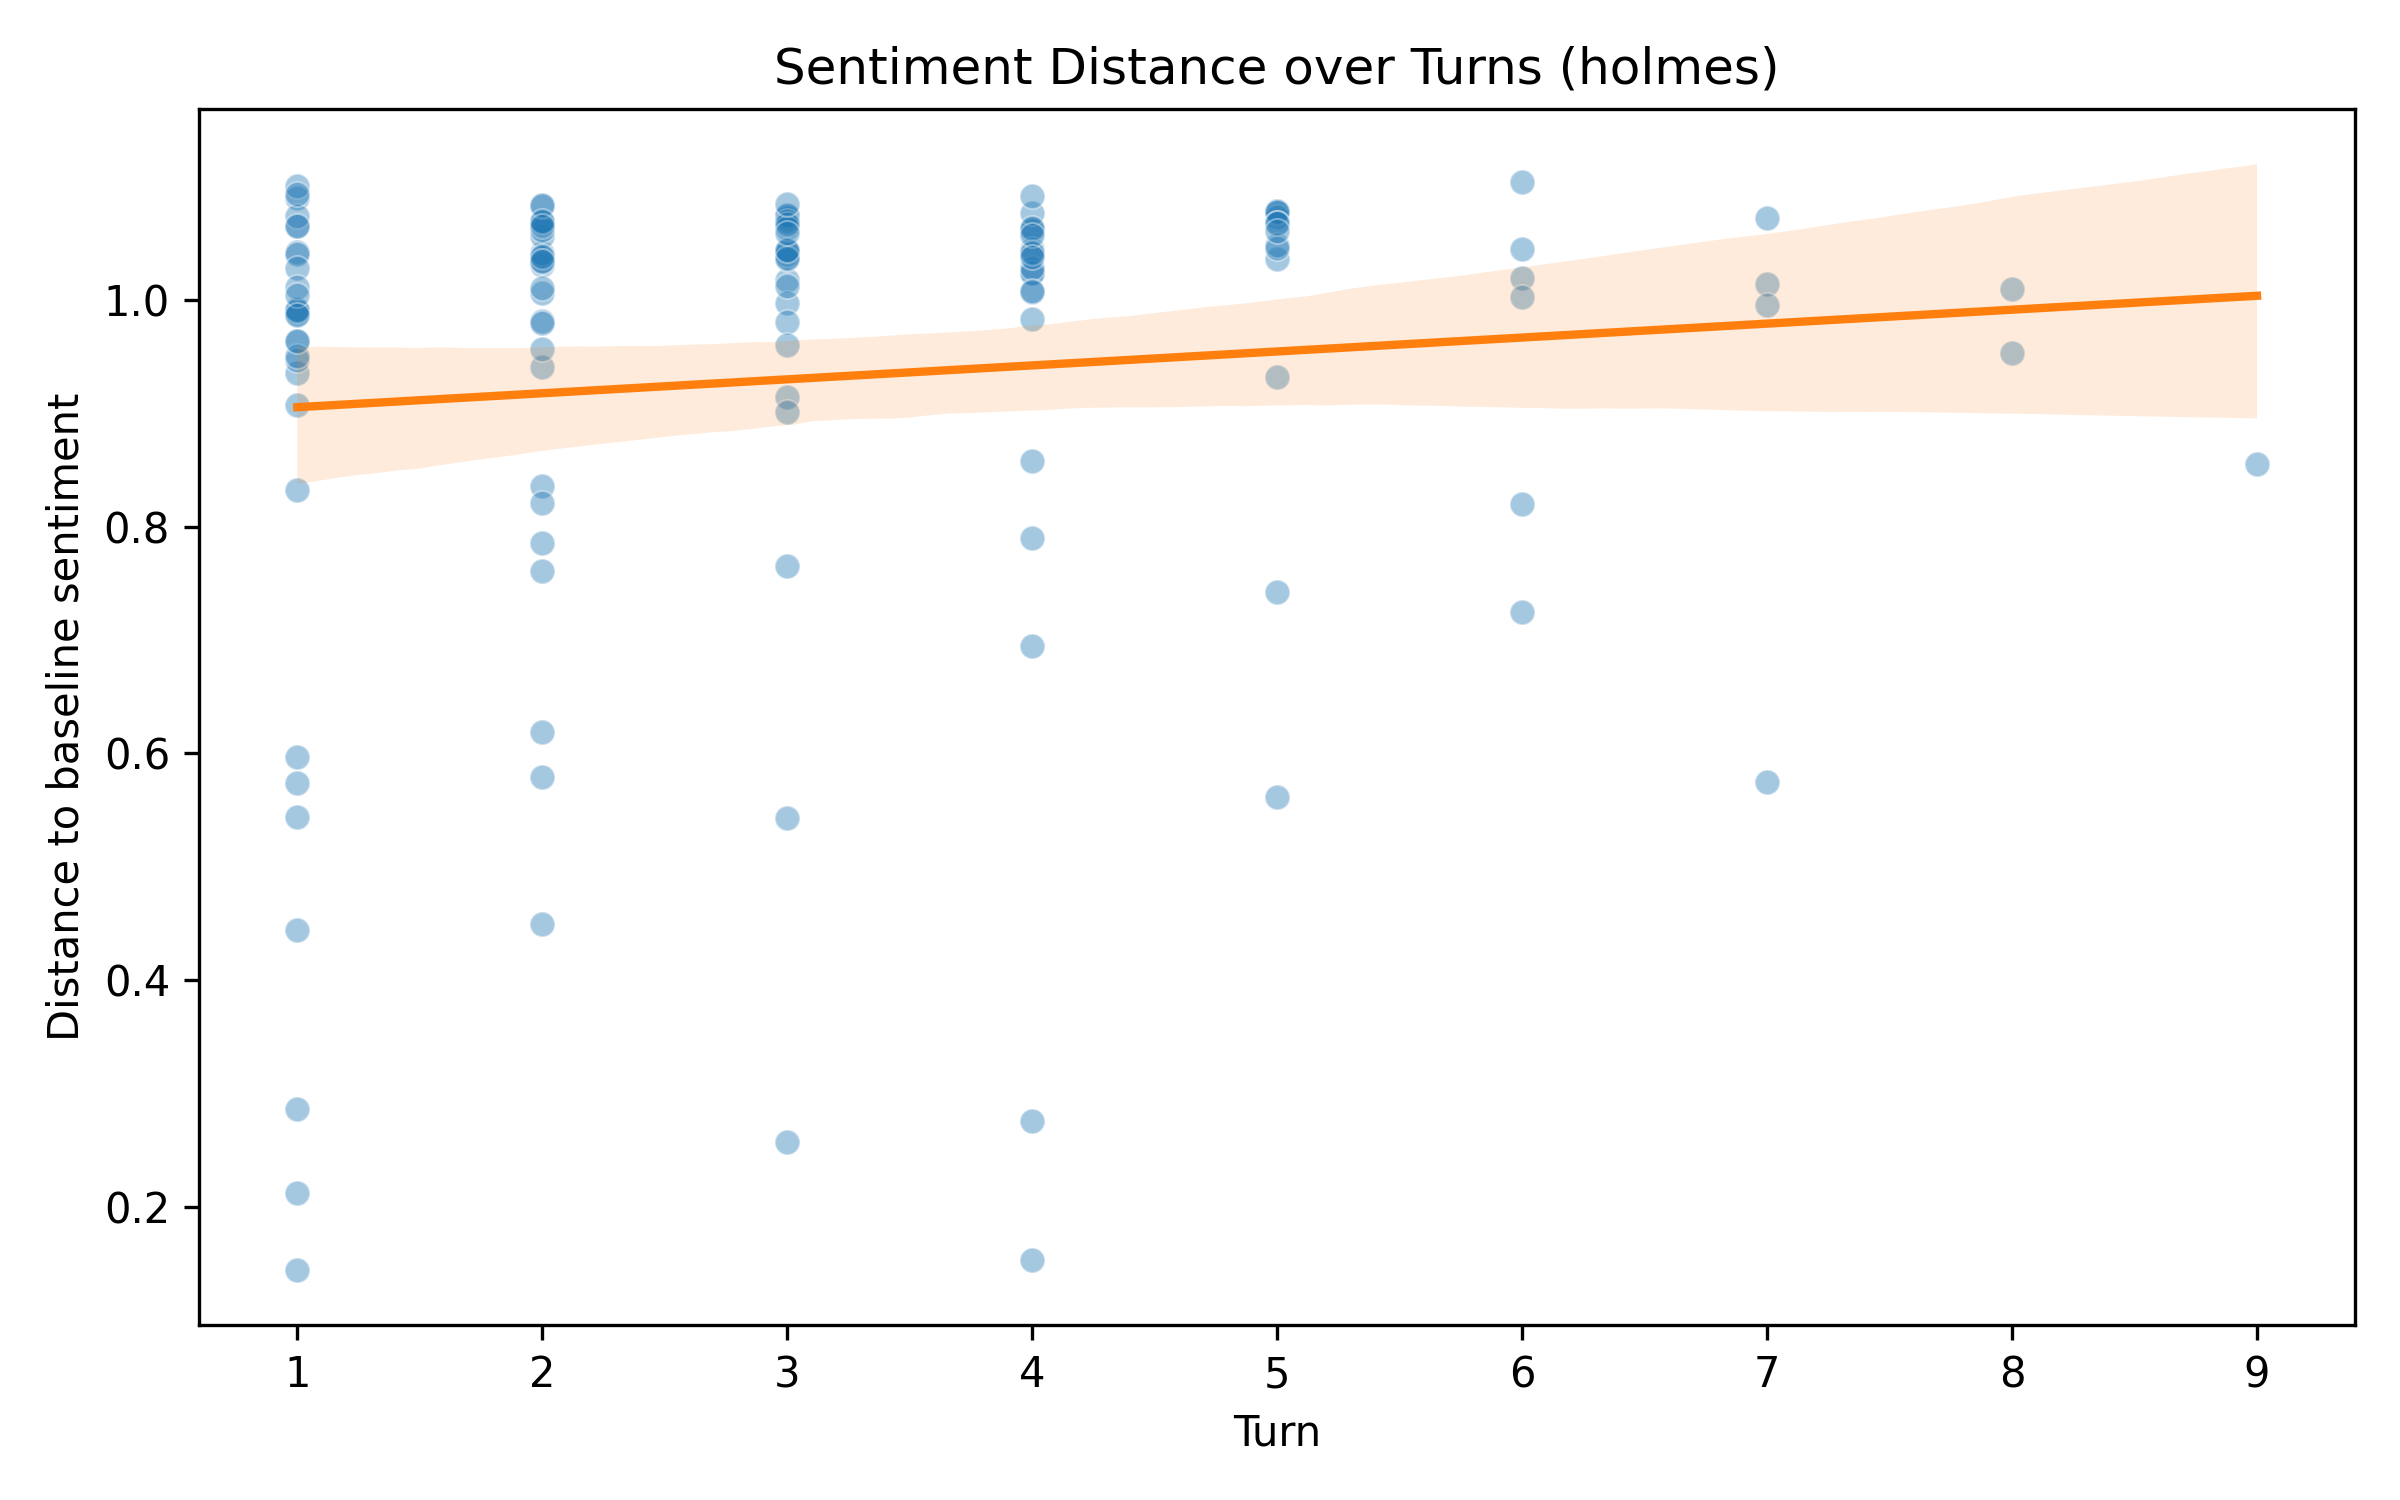
\includegraphics[width=.7\linewidth]{images/5.2_distance_over_turns_holmes.png}
            \caption{Holmes}\label{fig:vader_holmes}
        \end{subfigure}\qquad
        \begin{subfigure}[b]{1.2\textwidth}
            \centering
            
\includegraphics[width=.7\linewidth]{images/5.2_distance_over_turns_marple.png}
            \caption{Marple}\label{fig:vader_marple}
        \end{subfigure}
    \caption{Plot of Sentiment Distance Over Turns For Each Character}
    \label{fig:vader_1}
    \end{minipage}
\end{figure}

\begin{figure}[H]
    \centering
    \begin{minipage}{\textwidth}
        \centering
        \begin{subfigure}[b]{1.2\textwidth}
            \centering
             
\includegraphics[width=.7\linewidth]{images/5.2_distance_over_turns_poirot.png}
            \caption{Poirot}\label{fig:vader_poirot}
        \end{subfigure}\qquad
        \begin{subfigure}[b]{1.2\textwidth}
            \centering
            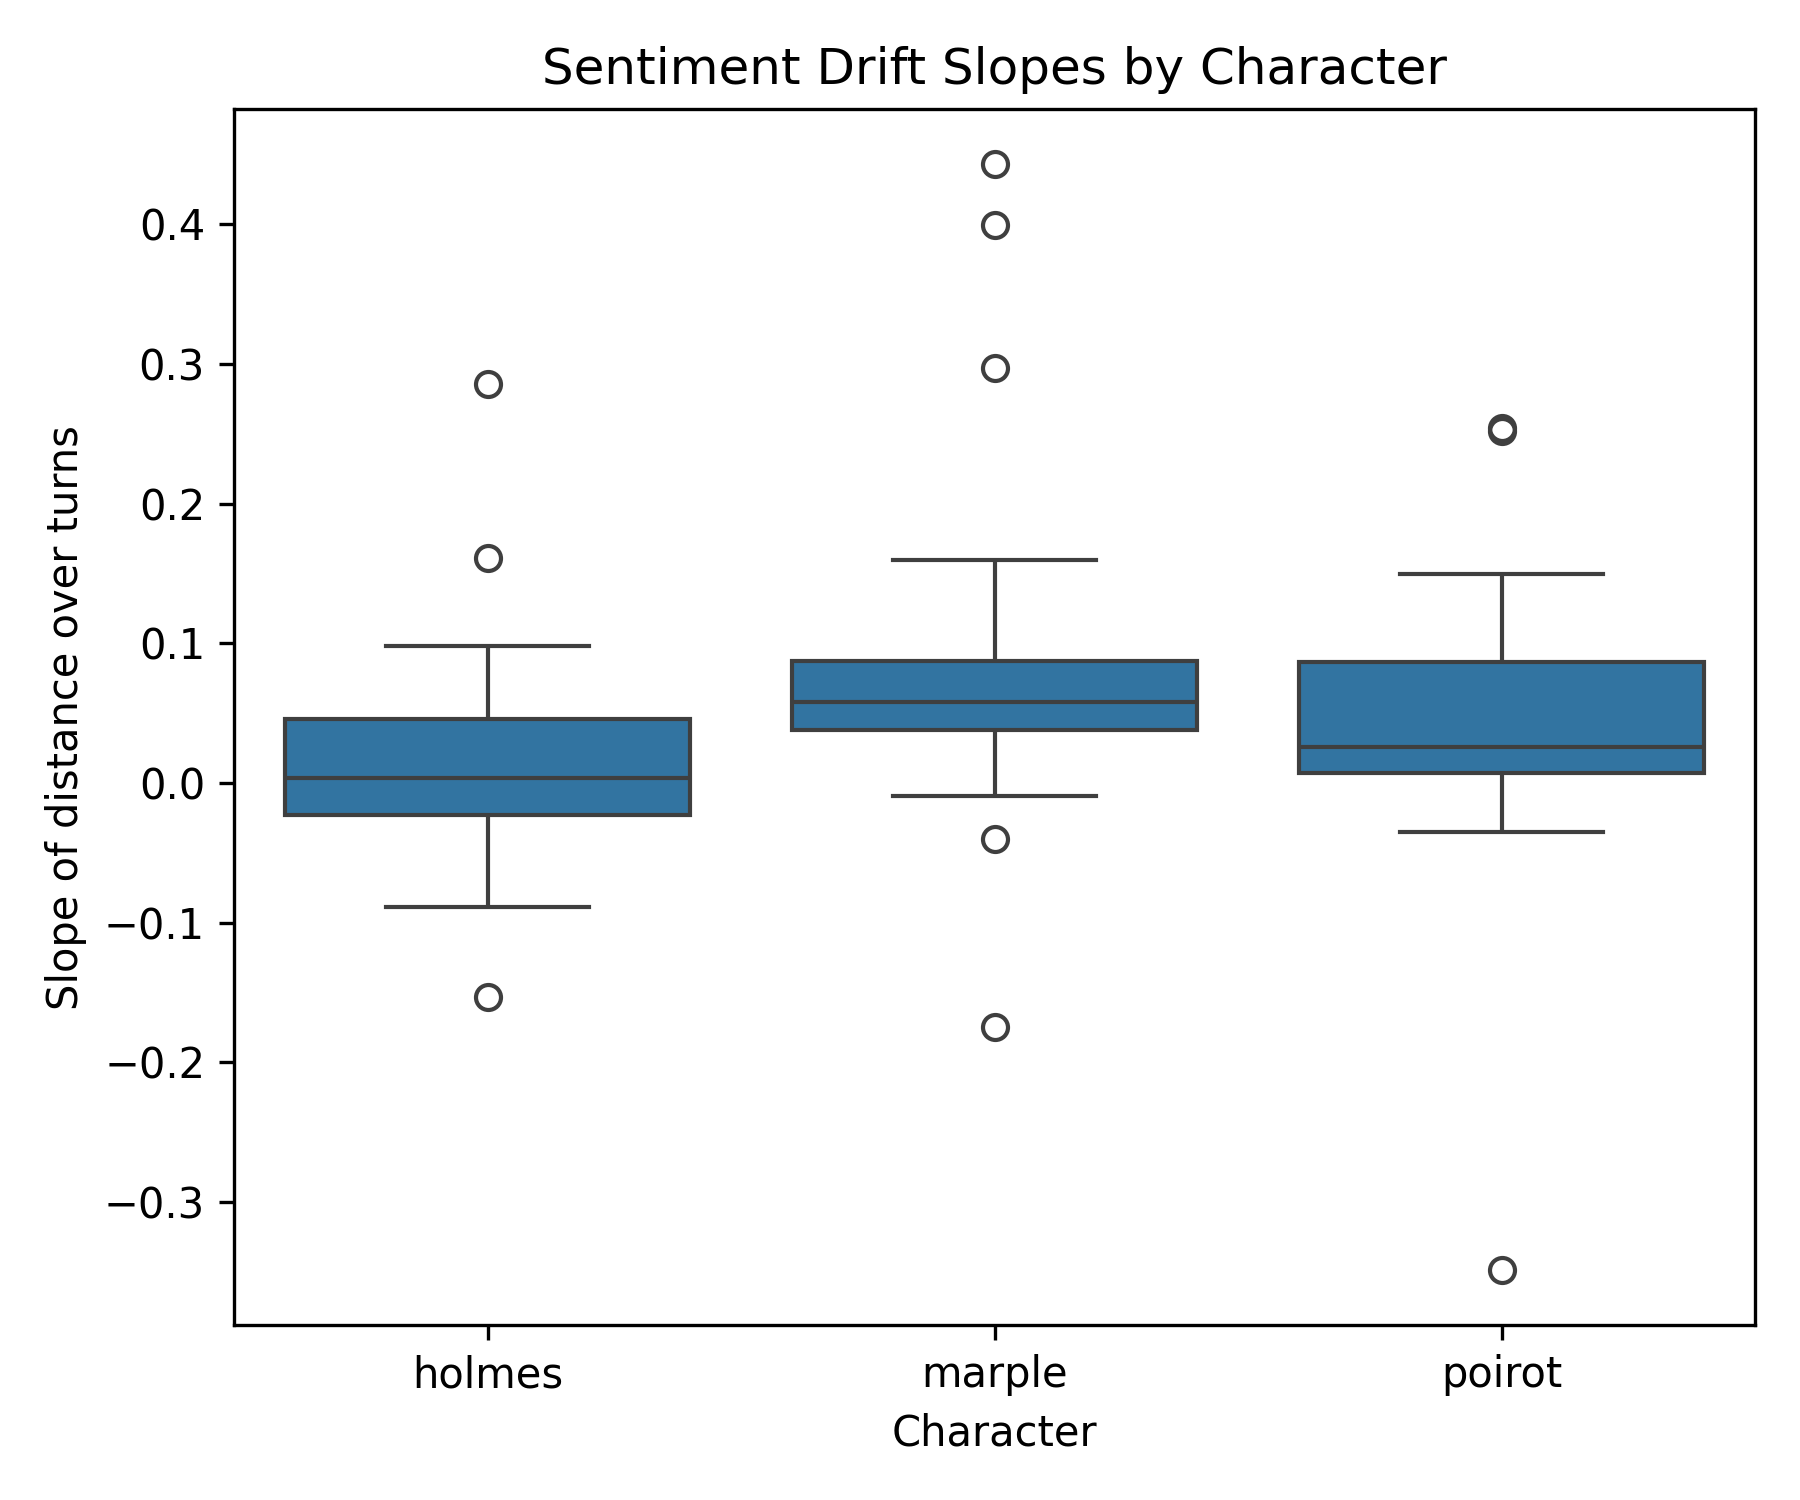
\includegraphics[width=.7\linewidth]{images/5.2_slope_boxplot_by_character}
            \caption{Boxplot}\label{fig:vader_boxplot}
        \end{subfigure}
    \caption{Plot of Sentiment Distance Over Turns For Each Character}
    \label{fig:vader_2}
    \end{minipage}
\end{figure}

\subsubsection{Alignment with literary affective baselines}

The numerical assessment first examined the mean sentiment features of the simulated dialogues. Table \ref{tab:sentiment_avg} summarised the average sentiment vectors for each detective across all simulations. The results indicated that simulated utterances were predominantly neutral, with all mean neutral scores exceeding 0.840. This concentration reflected the general tendency for large language models to produce affectively neutral text. Poirot demonstrated the highest level of neutrality (0.859) and the lowest compound sentiment (0.038), indicating a restrained discourse style in the simulations.

\begin{table}[H]
\centering
\begin{tabular}{l l l l l}\toprule
Character & Positive (pos) & Negative (neg) & Neutral (neu) & Compound \\\midrule
Holmes & 0.096 & 0.053 & 0.852 & 0.082 \\
Marple & 0.090 & 0.063 & 0.848 & 0.057 \\
Poirot & 0.084 & 0.057 & 0.859 & 0.038 \\ \bottomrule
\end{tabular}
\caption{Average sentiment vectors for each character}
\label{tab:sentiment_avg}
\end{table}


\subsubsection{Temporal trends in sentiment deviation}

The degree of discourse-level inconsistency was further quantified by the mean Euclidean distance and the slope of drift over turns. Table \ref{tab:sentiment_char} presented these indicators based on the character-level summary.

According to the results, Holmes maintained the largest mean distance ($M = 0.946$) from his literary baseline, indicating that his simulated persona was the most affectively distinct from the original source material. However, he also demonstrated the lowest mean slope ($M = 0.018$), suggesting that this deviation remained relatively constant throughout the interaction. In contrast, Marple showed the smallest initial mean distance ($M = 0.860$), suggesting a closer initial alignment with her literary reference. However, she also exhibited the steepest mean slope ($M = 0.083$) and the highest standard deviation in slopes ($SD = 0.122$). This indicated that while Marple begins closer to her canonical persona, her discourse consistency was the most prone to erosion over time. Poirot occupied a middle position in both mean distance ($M = 0.886$) and temporal drift ($M = 0.042$).


\begin{table}[H]
\centering
\begin{tabular}{l l l l l}\toprule
Character & Mean Slope & Std Slope & Mean Distance & Std Distance \\\midrule
Holmes & 0.018 & 0.081 & 0.946 & 0.144 \\
Marple & 0.083 & 0.122 & 0.860 & 0.110 \\
Poirot & 0.042 & 0.107 & 0.886 & 0.114 \\ \bottomrule
\end{tabular}
\caption{Character-Level Summary of Discourse Consistency Indicators}
\label{tab:sentiment_char}
\begin{flushleft}
\footnotesize
Note: One-way ANOVA testing differences in slope across characters: $F = 2.75$, $p = 0.070$. \\
Kruskal--Wallis test: $\chi^2 = 8.95$, $p = 0.011$ (significant at $\alpha = 0.05$).
\end{flushleft}
\end{table}

\subsubsection{Discourse results summary}

Although Marple's simulated dialogue aligned most closely with the affective profile of the baseline corpus, it suffered from the highest rate of character drift. Conversely, Holmes's affective profile was the most distant from the reference but remained the most stable over the course of the dialogue. These findings suggested that as collaborative reasoning progresses, agents tend to drift away from their specific literary personas toward a more generic, neutral discourse style, with the rate of this drift being character-dependent.


\subsection{Cross metric validation} \label{sec:results_validation}

To evaluate the reliability of the proposed character-consistency measures, each turn-level metric was compared with the classifier's probability of the correct character label. Correlation coefficients were computed to assess the association between linguistic measures and classifier confidence. In addition, expected calibration error (ECE) was calculated to examine the alignment between metric values and probabilistic predictions. The results are shown in Table \ref{tab:master_table}.

Correlation and ECE were computed using all available turn-level observations. Because intra-agent similarity requires a previous utterance, some metrics (for example, \texttt{character\_distance}) were not available for the first turn of each run, resulting in slightly smaller sample sizes for those metrics.


\begin{table}[h]
\centering
\begin{tabular}{l l l l l l l}\toprule
Metric & pearson\_r & spearman\_rho & ECE \\\midrule
lexical\_similarity & 0.353*& 0.384**& 0.226 \\
intra\_similarity & -0.084 & -0.161 & 0.195 \\
character\_distance & 0.018 & 0.102 & 0.130 \\
depth & -0.385**& -0.459***& 0.301 \\
z\_ref & -0.180 & -0.244*& 0.270 \\
z\_sim & -0.321*& -0.415***& 0.268 \\
sentiment\_distance & 0.183 & -0.016 & 0.551 \\ \bottomrule
\end{tabular}
\caption{Correlation between linguistic metrics and classifier-based character consistency}
\label{tab:master_table}
\end{table}


Lexical similarity showed a moderate and statistically significant positive association with classifier confidence (Pearson $r=0.353$; Spearman $\rho=0.384$). This indicated that stronger lexical alignment with the reference persona was associated with higher classifier-based character consistency. Among the evaluated measures, lexical similarity showed one of the clearest relationships with classifier predictions.

Syntactic depth showed the strongest correlation with classifier confidence (Pearson $r=-0.385$; Spearman $\rho=-0.459$). The negative direction indicated that increasing syntactic deviation from the reference style corresponded to lower classifier-based character consistency. The simulation-based syntactic deviation (\texttt{z\_sim}) also showed a significant negative association (Pearson $r=-0.321$), while the reference-based measure (\texttt{z\_ref}) showed a weaker relationship, reaching significance only under the Spearman correlation ($\rho=-0.244$). These results suggested that syntactic structure provided an important signal for character identification.

Sentiment distance did not show a statistically significant association with classifier confidence. Both linear and rank correlations remained weak, indicating limited alignment between sentiment variation and classifier-based character consistency. In this setting, discourse-level affect therefore played a relatively minor role in character recognition.



\subsubsection{Comparative faithfulness ranking}  \label{sec:results_validation_ranking}

To compare the overall reliability of the proposed measures, a composite faithfulness score was computed by combining normalised correlation strength (Pearson $r$ and Spearman $\rho$) with calibration alignment ($1-\text{ECE}$). The resulting ranking is shown in Table \ref{tab:ranking}.

Syntactic depth achieved the highest faithfulness score (0.864), followed by lexical similarity (0.837) and the simulation-based syntactic deviation (\texttt{z\_sim}; 0.799). These results indicated that lexical and syntactic features provided the most reliable signals of character consistency in the current evaluation framework. Reference-based syntactic deviation (\texttt{z\_ref}) showed moderate alignment (0.541), while transition-based metrics displayed weaker performance. Sentiment distance ranked lowest (0.150), suggesting that discourse-level affect contributed comparatively little to classifier-based character recognition in this setting.

\begin{table}[H]
\centering
\begin{tabular}{l l}\toprule
Metric& Faithfulness\_score\\\midrule
depth & 0.864 \\
lexical\_similarity & 0.837 \\
z\_sim & 0.799 \\
z\_ref & 0.541 \\
intra\_similarity & 0.450 \\
character\_distance & 0.398 \\
sentiment\_distance & 0.150 \\ \bottomrule
\end{tabular}
\caption{Faithfulness Ranking of Metrics}
\label{tab:ranking}
\end{table}


\subsection{Validation of character contamination} \label{sec:results_contamination}

To examine whether collaborative simulation alters character-specific representations, unsupervised clustering was applied to utterance embeddings produced by the fine-tuned classifier. The structure of simulation embeddings was compared with that of the reference corpus.

K-means clustering ($k=3$) was applied separately to both datasets. For the reference corpus, five bootstrap samples were drawn to match the number of simulation utterances, which explains the multiple reference rows in Table~\ref{tab:clustering}. Cluster quality was evaluated using the silhouette coefficient, cluster purity, and the adjusted Rand index (ARI). For the reference corpus, $\mathrm{ARI_{case}}$ is not defined, as no case structure is present.


\begin{table}[H]
\centering
\begin{tabular}{l l l l l l}\toprule
Data\_type& silhouette & purity & ARI\_character & ARI\_case \\\midrule
reference (bootstrap 1) & 0.3437 & 0.8889 & 0.6970 & NaN \\
reference (bootstrap 2) & 0.3163 & 0.8837 & 0.6846 & NaN \\
reference (bootstrap 3) & 0.3368 & 0.8708 & 0.6626 & NaN \\
reference (bootstrap 4) & 0.3266 & 0.8837 & 0.6885 & NaN \\
reference (bootstrap 5) & 0.2973 & 0.8708 & 0.6546 & NaN \\
simulation & 0.4064 & 0.4005 & 0.0070 & 0.0269 \\ \bottomrule
\end{tabular}
\caption{Clustering performance on reference and simulation embeddings}
\label{tab:clustering}
\end{table}

In the reference corpus, clustering results showed clear alignment with character identity. Across bootstrap samples, silhouette values ranged from 0.30 to 0.34, indicating moderate separation between clusters. Cluster purity remained high (0.87-0.89), and ARI with respect to character labels ($\mathrm{ARI_{character}}$) ranged from 0.65 to 0.70, showing strong agreement between clusters and true identities. These results indicate that the embedding space preserved character-specific structure in the reference data.

In the simulation data, embeddings were derived from the same classifier, but clustering showed a different pattern. The silhouette coefficient increased to 0.41, suggesting that clusters were still well separated in the embedding space. However, cluster purity dropped to 0.40, and ARI with respect to character labels fell to near zero (0.007). ARI with respect to case labels was also close to zero (0.027), indicating that clusters did not correspond to either character identity or case structure.

Taken together, these results show that although clustering structure remained, it no longer reflected meaningful labels. High silhouette with low ARI and purity indicates that the embedding space was organised along dimensions that do not correspond to character identity. This suggests that collaborative simulation reduced the distinctiveness of character representations, leading to substantial overlap between characters.

Overall, the clustering analysis provides evidence of character contamination. Compared with the reference corpus, simulated dialogue showed a marked reduction in the separability of character-specific features in the embedding space.


\section{Discussion} \label{sec:discussion}

\subsection{Overview of findings}

This section provides a summary of the experimental results and directly addresses the research questions of this study (Subsection\ref{sec:intro_rq}). The findings provided substantial evidence for the proposed hypotheses, while also revealing complex dynamics in character consistency within collaborative mystery murder game task.

Regarding \emph{RQ1}, the results supported the hypothesis that large language models (LLMs) only partially maintained their assigned personas during collaborative reasoning tasks. While the agents successfully adopted initial character identities, significant character inconsistency and contamination emerged over the course of the interaction. The classifier-based baseline revealed significant negative temporal trends in attribution confidence for specific character-case combinations, such as Holmes in Case 1 and Marple in Case 3 (Subsection \ref{sec:results_classifier}). Furthermore, the clustering analysis demonstrated that the distinctiveness of character representations declined during the simulation, leading to a substantial overlap between the agents (Subsection \ref{sec:results_contamination}). This confirmed that the pressure of multi-agent collaboration caused agents to mirror each other's styles and drift toward a uniform, generic "AI register".

For \emph{RQ2}, the investigation validated the hypothesis that a multi-level linguistic framework provides a more comprehensive assessment of character consistency than any single metric. The different levels of analysis captured distinct facets of character erosion. At the lexical level, Poirot demonstrated the strongest and most stable alignment with his reference vocabulary, while Marple's character distance score was near zero, indicating her lexical choices were highly susceptible to the collective dialogue flow (Subsection \ref{sec:results_lexical}). However, the syntactic level revealed a different pattern: all characters, including those lexically stable, exhibited a significant global increase in structural complexity compared to their literary references
(Subsection \ref{sec:results_syntactic}). Systematic erosion was observed as sentences became increasingly complex over turns for Holmes and Poirot. At the discourse level, all agents drifted away from their specific affective profiles toward a neutral style (Subsection \ref{sec:results_discourse}). These inconsistent conclusions across dimensions—where a character might appear consistent lexically but fail syntactically—justified the necessity of a layered perspective to track the micro-level breakdown of persona.

Finally, \emph{RQ3} addressed the reliability of these metrics through validation against the classifier-based scores. The results identified Syntactic depth as the most reliable metric, achieving the highest composite faithfulness score (0.864). Lexical similarity also showed a significant positive association with classifier confidence, whereas sentiment distance played a minor role in character recognition. These findings established a validated hierarchy of metrics for monitoring character stability in role-playing LLM agents.

\subsection{Trade off Between persona and performance}

Previous studies have shown that multi-agent interaction can support collective reasoning but may also reduce the stability of character representations \citep{baltaji2024cultured, choi2024examining}. Similar patterns have been observed in generative agent systems, where social interaction altered internal representations and reduced character-specific detail \citep{xiao2023simulating}.

The experimental results demonstrated a clear trade-off between solving the mystery and maintaining character consistency. Case-solving rates under the three experimental conditions highlighted this tension. The zero-shot baseline (C1) achieved near-perfect accuracy (97\%-100\%). When persona constraints were introduced (C2), performance declined, and collaborative interaction (C3) caused a further drop (Subsection \ref{sec:results_case-solving-rate}). This confirmed that maintaining character over multiple turns can interfere with logical reasoning, consistent with prior work suggesting that sustained persona effort reduces task performance \citep{shao2023characterllm, xiao2023policy, xiao2023simulating}. Under collaboration, agents prioritised group consensus over individual accuracy, sometimes abandoning their assigned viewpoints to conform \citep{baltaji2024cultured}.

Performance in the collaborative condition (C3) was notably lower than in C1 or C2. Agents frequently sacrificed their personal investigative strategies or distinctive traits to maintain harmony, sometimes failing to voice dissenting opinions. As a result, the dialogue context and history became a stronger influence than the initial persona prompt, and task-oriented cooperation tended to override individual character features \citep{shanahan2023role, xiao2023simulating, chen2024socialbench}.

The progressive decline in accuracy from C1 to C3 suggested that current LLMs struggled to handle complex social reasoning without reducing logical reasoning and task performance \citep{ji2025enhancing}. The findings provide empirical evidence for a performance-persona trade-off, namely enforcing character consistency can hinder task performance, especially in collaborative multi-agent settings.

\subsection{Character contamination}

The clustering analysis indicates a substantial decline in character consistency at the global representational level. In the reference corpus, the three detectives occupy distinct regions in the embedding space, as reflected by high cluster purity and strong alignment with character labels. 

In the simulation data, this alignment was largely reduced. Although clustering structure remained, it no longer corresponds to character identity. This was reflected in the near-zero ARI ($\mathrm{ARI_{character}}$ = 0.007) and the substantial drop in purity (from 0.88 in the reference corpus to 0.40 in the simulation), indicating that cluster assignments were no longer consistent with the true character labels.

This pattern suggests that while the embedding space still contained separable structure, the dimensions organising this structure were no longer character-specific. As a result, the overall linguistic fingerprints of the characters became less distinct, consistent with the notion of character contamination, where identity boundaries are weakened in collaborative settings \citep{choi2024examining, bao2026eval4sim}.


\subsection{Character-dependent variations in consistency}

The results demonstrated that character consistency was not uniform across the three agents, suggesting that the stability of a persona depends on the distinctiveness of its linguistic markers. Poirot exhibited the highest level of robustness, maintaining stable lexical features and classifier confidence even under the pressure of collaboration (Subsection \ref{sec:results_classifier_poirot}, \ref{sec:results_lexical}). This stability likely stemmed from the salience of his linguistic anchors such as the specific blend of French-English vocabulary and methodical, third-person discourse, these provided the model with a highly differentiated template that was less susceptible to environmental noise.

In contrast, Marple proved to be the most vulnerable to character contamination. While her individual utterances appeared consistent in isolation, her character distance score was near zero, indicating that her linguistic choices became indistinguishable from the collective dialogue flow. This vulnerability can be attributed to the overlap between her assigned persona (characteristic politeness, hedging, and indirectness) and the generic "AI register" (overly polite, civil, and neutral) \citep{shanahan2023role}. Consequently, as the interaction progressed, the boundaries of her identity blurred, leading to the highest rate of sentiment drift observed in the study (Subsection \ref{sec:results_discourse}).

Holmes presented a different pattern of inconsistency, characterised by a stable but distant affective profile (Subsection \ref{sec:results_discourse}). Although he maintained a unique lexical fingerprint, his utterances consistently showed the largest deviation from the literary baseline's emotional tone. This suggests a conflict between character traits and task requirements. Holmes's canonical "cold detachment" and "lack of interest in social norms" are fundamentally at odds with the collaborative nature of the mystery-solving task, which requires active perspective-taking and communicative cooperation. The observed decline in classifier confidence for Holmes (Subsection \ref{sec:results_classifier_holmes}) indicates that when faced with the dual demand of social reasoning and character performance, the model prioritised task-relevant cooperation over the maintenance of an abrasive or detached persona. 
 
These findings imply that a LLM agent's ability to stay in character might be constrained by how well the character's linguistic fingerprints align with both the model's pre-trained biases and the social dynamics of the environment.


\subsection{Methodological contributions}

The primary methodological contribution of this research is the development of a multi-dimensional framework grounded in linguistic theory. Many existing studies evaluate character consistency using macro-level indicators, such as task success, human judgment, or abstract personality tests. While these methods offer useful insights into an agent's general behaviour, they often overlook how a character is actually performed through specific language use. This thesis addresses this gap by examining character consistency across three distinct layers: lexical patterns, syntactic structures, and discourse-level affect. By focusing on these micro-level features, the framework can detect subtle shifts in character behaviour that are often invisible to broader behavioural assessments. 

Furthermore, this approach provides a more detailed view of how character consistency evolves over time. Instead of relying on a single aggregate score, the multi-level analysis reveals that an agent can maintain its identity in one dimension while losing it in another. For example, Marple achieved moderate lexical alignment with her literary reference, yet the more detailed character distance metric revealed that her linguistic choices were almost indistinguishable from the collective dialogue flow. Similarly, while Poirot demonstrated the strongest and most stable alignment with his reference vocabulary, the syntactic analysis revealed a significant global increase in structural complexity that drifted further from the literary baseline. This distinction is critical for understanding the complex dynamics of role-playing in multi-agent environments.

Finally, this framework moves beyond task-specific outcomes to offer an intrinsic evaluation of character performance. High task accuracy does not always mean an agent is remaining in character, as a model may solve a problem by abandoning its assigned persona to be more efficient. By prioritising linguistic form over task performance, this methodology offers a more rigorous way to evaluate the authenticity of LLM simulations. This shift from macro-evaluations to micro-linguistic analysis provides a valuable tool for future researchers seeking to build more resilient and believable role-playing agents.

\subsection{Limitations and future work}

Several limitations should be acknowledged when interpreting the findings of this study. First, the construction of the gold-standard corpus and the classifier involved specific design choices that may have introduced bias. The character utterances used for training were extracted via an LLM-assisted pipeline, which may have contained attribution errors or noise from the original texts. Furthermore, while the classifier was trained on an 80\% split of the literary data, the subsequent comparison of lexical and syntactic metrics used the entire 100\% dataset as a reference. This overlap between the training data of the validator and the reference points for the metrics could have led to a slight overestimation of alignment. Additionally, two of the selected detectives, Poirot and Marple, were created by the same author (Agatha Christie). It is possible that shared authorial style and linguistic habits created an underlying similarity between these two personas that the current metrics could not fully separate from character-specific traits.

Second, the scope of the simulation data and the sampling methods limit the generalisability of the findings. The analysis was based on a sample of 100 filtered utterances for several linguistic metrics to ensure computational efficiency. A larger sample size, or the inclusion of the entire generated corpus, might have revealed different patterns of erosion. Moreover, the experiment used only three specific murder mystery cases. The results suggested that character consistency was often case-dependent, as seen in the significant decline of Holmes's consistency only in Case 1. Future research should involve a broader range of scenarios and perform case-specific analyses to determine how different narrative contexts influence character performance.

Third, the scope of this research was confined to three specific literary figures and a single model architecture, namely Llama-3.2-3B-Instruct. As a result, the patterns observed here—such as the high reliability of syntactic indicators—might vary when applied to characters with less distinctive voices or when using larger, more complex language models. In addition, the simulation involved only three agents interacting in each run. The dynamics of character consistency could differ in settings with more agents or with different group sizes.

Moreover, the theoretical assumption that "linguistic fingerprints" are a valid proxy for character consistency requires further validation. While this research focused on observable language patterns, the relationship between these micro-linguistic features and a deeper, stable "persona" remains complex. Future work could incorporate standard psychological metrics or personality tests as an additional layer of validation. This would allow for a comparison of how linguistic drift correlates with shifts in an agent's underlying psychological profile.

Finally, there are limitations regarding the implementation of the prompting and the linguistic metrics. The current agent construction relied on specific choices for character prompts, task presentation, and memory management. Although these choices were informed by prior literature, the robustness of the results to different prompting strategies was not tested. Similarly, the linguistic metrics used in this study represent a first proof of concept. The analysis focused on basic lexical similarity and syntactic depth, but more advanced measures—such as dependency tree structures for syntax, topic modelling for discourse, or advanced embedding methods for semantics—could provide deeper insights. Future studies could also employ different sentiment classification models or more nuanced discourse markers to further refine the measurement of character-level affect.



\section{Conclusion} \label{sec:conclusion}

This thesis investigated character consistency in multi-agent large language model (LLM) collaboration through a novel, linguistically grounded evaluation framework. By simulating three iconic detectives (Sherlock Holmes, Hercule Poirot, Miss Marple), the research addressed how well agents maintain their personas during collaborative reasoning and which linguistic metrics most accurately track these changes. The results showed that LLMs only partially maintained their assigned personas. Significant character inconsistency and contamination emerged as the interactions progressed, with the agents' unique linguistic fingerprints eventually converging into a uniform, undifferentiated group style. A clear performance-persona trade-off was identified: as persona constraints and collaborative requirements were introduced, the agents' ability to solve the cases declined. This suggested that the cognitive burden of maintaining a complex character can interfere with logical reasoning and task success.

Character-specific variations were also prominent. Poirot exhibited the most robust consistency, likely due to his highly distinct linguistic anchors. In contrast, Marple proved most vulnerable to character drift, as her polite and indirect style often merged with the neutral, standardised language of the model. Holmes maintained a unique lexical style but displayed significant affective distance from his literary reference, prioritising task-relevant cooperation over his canonical detached persona.

The multi-level linguistic framework proved effective for capturing these subtle shifts. Among the various metrics, syntactic depth was identified as the most faithful and reliable indicator of character consistency, followed by lexical similarity. Discourse-level sentiment analysis, while useful for tracking affective drift, was found to be the least reliable for character recognition in this setting.

In conclusion, the findings demonstrated that collaborative dynamics significantly challenge character consistency of LLM agents. The development of this linguistic grounded multi-dimensional evaluation methodology offers a scalable way to monitor and validate character performance in complex social applications.


% ------ 引用 ------
\bibliographystyle{plainnat}
\bibliography{custom}




% ------ 附录 ------
\begin{appendices} \label{sec:app}


\section{Glossary of Key Concepts}
\begin{description}

\item[Character]
The identity as realised through linguistic behaviour in dialogue.

\item[Persona] 
The explicitly assigned profile or identity specification provided to the model through prompting.

\item[Character Consistency]
The successful maintenance of a specific linguistic style over the course of an
interaction.


\item[Character Hallucination]
The phenomenon that agents solve the case based on memorised plots instead of collaborative reasoning.

\item[Character Contamination] 
The blurring of identity boundaries within multi-agent collaboration, where the pressure of collaboration may cause agents to unconsciously mirror each other's linguistic style.

\item[Character Modelling]
Conditioning a language model on a character description namely the persona. It has evolved from simple prompt engineering to complex architectural fine-tuning and specialised training. 

\item[Simulation]
A complete run of the case, terminates when 10 maximum turns are reached or a mutual agreement on the murderer's identity is reached.

\item[Turn]
A complete cycle in which all three agents each speak once in a randomly determined order. 

\item[Utterance]
A single agent's complete response in one turn of the dialogue, which may contain multiple sentences.

\item[Linguistic Fingerprint] 
the unique pattern of language that defines a specific character's voice and acts as a measurable sign of their identity stability.

\item[Jubensha]
A Chinese live action role-playing murder mystery game (also know as script murder games).

\end{description}



\section{Prompt for generating role-play guideline} \label{sec:app_gen_persona}

\section{Role-Play Guideline} \label{sec:app_char_prompt}

\subsection{Holmes}
    \inputminted{yaml}{../prompts/holmes.yaml}

\subsection{Marple}
    \inputminted{yaml}{../prompts/marple.yaml}
    
\subsection{Poirot}
    \inputminted{yaml}{../prompts/poirot.yaml}


\section{Background and Collaboration Rule} \label{sec:app_rule_prompt}
    \inputminted{yaml}{../prompts/rule_collab.yaml}


\section{Case Data} \label{sec:app_case}

\subsection{Case 1} \label{sec:app_case1}
    \inputminted{yaml}{../cases/case1.yaml}
\subsection{Case 2} \label{sec:app_case2}
    \inputminted{yaml}{../cases/case2.yaml}
\subsection{Case 3} \label{sec:app_case3}
    \inputminted{yaml}{../cases/case3.yaml}

\section{Prompt for generating profiles} \label{sec:app_gen_profile}
    \inputminted{yaml}{../prompts/profile_prompts.yaml}

\section{Generated Character Descriptions} \label{sec:app_char_dcp}

\subsection{Character Description of Holmes} \label{sec:app_dcp_holmes}
    \inputminted{text}{../profiles/sherlock_holmes_analysis.txt}
\subsection{Character Description of Marple} \label{sec:app_dcp_marple}
    \inputminted{text}{../profiles/miss_marple_analysis.txt}
\subsection{Character Description of Poirot} \label{sec:app_dcp_poirot}
    \inputminted{text}{../profiles/hercule_poirot_analysis.txt}


\section{List of Source Texts} \label{sec:app_novels}
The following literary works were used as the literary corpus for classification model training and also the gold corpus for analysis.

\subsection{Sherlock Holmes (Arthur Conan Doyle)}
\begin{itemize}[itemsep=0pt, parsep=0pt, topsep=2pt, partopsep=0pt]
    \item Doyle, A. C. \textit{A Study in Scarlet}
    \item Doyle, A. C. \textit{The Adventures of Sherlock Holmes}
    \item Doyle, A. C. \textit{His Last Bow}
    \item Doyle, A. C. \textit{The Case-Book of Sherlock Holmes}
    \item Doyle, A. C. \textit{The Memoirs of Sherlock Holmes}
    \item Doyle, A. C. \textit{The Return of Sherlock Holmes}
    \item Doyle, A. C. \textit{The Valley of Fear}
    \item Doyle, A. C. \textit{The Hound of the Baskervilles}
    \item Doyle, A. C. \textit{The Sign of the Four}
\end{itemize}

\subsection{Miss Marple (Agatha Christie)}
\begin{itemize}[itemsep=0pt, parsep=0pt, topsep=2pt, partopsep=0pt]
    \item Christie, A. \textit{A Pocket Full of Rye}
    \item Christie, A. \textit{The Mirror Crack'd from Side to Side}
    \item Christie, A. \textit{The Complete Short Stories of Miss Marple}
    \item Christie, A. \textit{Sleeping Murder}
    \item Christie, A. \textit{The Body in the Library}
    \item Christie, A. \textit{Nemesis}
    \item Christie, A. \textit{The Moving Finger}
    \item Christie, A. \textit{The Thirteen Problems}
    \item Christie, A. \textit{At Bertram's Hotel}
    \item Christie, A. \textit{They Do It with Mirrors}
    \item Christie, A. \textit{A Murder Is Announced}
    \item Christie, A. \textit{The Murder at the Vicarage}
    \item Christie, A. \textit{A Caribbean Mystery}
    \item Christie, A. \textit{Miss Marple's Final Cases}
    \item Christie, A. \textit{4.50 from Paddington}
\end{itemize}

\subsection{Hercule Poirot (Agatha Christie)}
\begin{itemize}[itemsep=0pt, parsep=0pt, topsep=2pt, partopsep=0pt]
    \item Christie, A. \textit{The ABC Murders}
    \item Christie, A. \textit{Murder in Mesopotamia}
    \item Christie, A. \textit{Death on the Nile}
    \item Christie, A. \textit{Cards on the Table}
    \item Christie, A. \textit{The Murder of Roger Ackroyd}
    \item Christie, A. \textit{Murder on the Orient Express}
    \item Christie, A. \textit{Mrs McGinty's Dead}
    \item Christie, A. \textit{Five Little Pigs}
    \item Christie, A. \textit{Lord Edgware Dies}
    \item Christie, A. \textit{Hercule Poirot's Christmas}
    \item Christie, A. \textit{Evil Under the Sun}
    \item Christie, A. \textit{Halloween Party}
\end{itemize}
\end{appendices}
% ----------------



\end{document}
